\documentclass[a4paper,10pt]{problems}

\begin{document}

{\makerusother\relax
\immediate\write\tsk{\noexpand\epigraph{\noexpand\dotsупражнений, которые настоятельно и, как всегда, 
безуспешно, рекомендую делать\noexpand\dots}{}}
}

\Header{Динамическое программирование}

\begin{flushright}
Автор: Петр Калинин, основной текст: 2008\\
Этот документ можно распространять по лицензии\\
Creative Commons Attribution-ShareAlike 3.0 Unported (CC BY-SA 3.0)\\
Последнюю версию, а также исходный код для системы \LaTeX\\
можно скачать с \verb`https://github.com/petr-kalinin/progtexts`\\
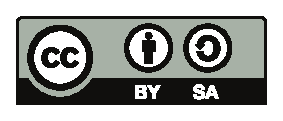
\includegraphics[width=2cm]{by-sa-corr.eps}
\end{flushright}

\epigraph{
    Динамическое программирование "--- это когда у нас
    есть одна большая задача, которую непонятно как решать,
    и мы разбиваем ее на меньшие задачи, которые тоже
    непонятно как решать.\\
    А.""С. Кумок
}

Динамическое программирование (ДП, динамика) "--- это \textit{метод} решений задач совершенно разных классов. 
Пожалуй, это единственный в своём роде раздел олимпиадного программирования: не алгоритм, не 
структура данных, а именно метод, идея решения задач. {\footnotesize К динамической памяти он, 
конечно, отношения не имеет.}

ДП идейно очень напоминает метод математический индукции. Это очень полезно держать в голове при 
чтении дальнейшего текста, тогда, может быть, все будет проще.

Может показаться, что ДП "--- это некий чёткий алгоритм построения решения задачи, т.е.
что достаточно его освоить "--- и все соответствующие задачи будут решаться с ходу, без 
затруднений. Конечно, это не так; в любых задачах всегда приходится хоть немного, но думать
головой. Поэтому смотрите на все, что я тут написал, как на то, что поможет вам в этом думании;
в каждой конкретной задаче могут возникнуть дополнительные особенности и т.п.

\header{Элементарные примеры}

\epigraph{Конечно, подобная тема очень обща и поневоле располагает к философствованию "--- 
начинаешь говорить так расплывчато, что понять тебя может всякий\dots Я постараюсь говорить конкретнее, ибо считаю,
что простая мысль, но выраженная честно, полезнее туманных намёков. Поэтому в первой лекции, не 
вдаваясь в общие рассуждения, я просто расскажу об одном физическом законе, дабы вы имели хоть один 
пример того, о чем впоследствии пойдёт отвлечённый разговор.}{Ричард Фейнман. Характер физических 
законов.}

Сначала разберём три примера задач на ДП. Именно на этих примерах дальше я и буду показывать 
различные общие идеи ДП.

\lheader{Задачи про черепашку} (Не знаю, почему принято формулировать эти задачи именно с 
упоминанием черепашки, но такая традиция.) Есть клетчатое поле $N\times M$. В левом нижнем углу 
сидит черепашка. Она умеет ходить только вправо или вверх. а) Сколько у неё разных путей до правого 
верхнего угла? б) В каждой клетке поля записано некоторое число. Требуется найти максимальную сумму чисел, 
которую можно набрать по пути в правый верхний угол (для начала не будем обсуждать, как найти 
\textit{путь}, на котором сумма будет максимальна, а будем искать только саму эту \textit{сумму}).

Как будем решать эти задачи? \textsc{Первая основная идея ДП:} будем искать ответ не только на нашу 
общую задачу, но и \textit{на более мелкие аналогичные задачи} ("<подзадачи">). В данном случае: решим не только нашу 
задачу, а вообще для каждой клетки поля найдём а) сколько способов до неё добраться; б) какую 
максимальную сумму можно собрать по дороге к этой клетке.

Ну и что? А как эти-то задачи решить? Ну, есть одна подзадача, для которой ответ очевиден. До левого 
нижнего угла а) есть только один способ добраться; б) как ни крути, а сумма, которую при этом 
наберёшь, равна числу, записанному в этом самом нижнем левом угле.\footnote{Не знаю, как вам, а мне 
всегда хочется в этой задаче спросить: а считается в сумме только числа в тех клетках, на которые 
черепашка \textit{переходит}, т.е. без начальной "--- или во всех вообще, считая начальную? Можете 
подумать, почему для идеи решения задачи это абсолютно все равно и чем будут отличаться алгоритмы 
решения того и того; а мы дальше будем считать, что учитываются все клетки.} Далее, для клеток 
левого столбца и нижней строки тоже все очевидно.  
\taskn{Контрольный вопрос}|Как найти ответы на эти подзадачи?||||Очевидно: до этих клеток есть только один способ добраться, и потому а) $ans[1,j]=ans[i,1]=1$; б) $ans[1,j]$ и $ans[i,1]$ равен сумме всех чисел по пути от начальной до этой клетки.|
А остальные клетки? Решая задачу для очередной клетки, будем считать, что мы уже знаем ответ для 
предыдущих клеток и попробуем, используя это знание, найти ответ и для текущей. А для этого 
\textsc{Вторая основная идея ДП:} \textit{а на что может заканчиваться} любое
решение этой подзадачи? В данном случае все очевидно: либо мы только что сходили вправо, либо 
только сходили вверх. (Обратите внимание, что первый столбец и первую строку мы уже разобрали, 
поэтому оба варианта "--- и ход вправо, и ход вверх "--- теперь возможны.) Если немного 
подумать, то отсюда ясно, что ответ на нашу текущую подзадачу можно легко выразить через ответы на 
две подзадачи: на подзадачу для клетки слева от текущей и на подзадачу для клетки снизу. В варианте 
а) ответ для клетки $(i,j)$ будет, очевидно, равно сумме ответов для клеток $(i-1,j)$ и $(i,j-1)$ 
(считаем столбцы занумерованы слева направо, а строки "--- снизу вверх); в варианте б) ответ для 
клетки $(i,j)$ будет, очевидно, равен максимуму из ответов для клеток $(i-1,j)$ и $(i,j-1)$ плюс 
собственно значение, записанное изначально в клетке $(i,j)$. Короче говоря,
$$
\mbox{а) }ans[i,j]=ans[i-1,j]+ans[i,j-1]; 
\qquad\mbox{б) }ans[i,j]=max(ans[i-1,j],ans[i,j-1])+a[i,j],
$$
где в варианте б) $a$ "--- массив, в котором храним числа, изначально записанные в клетках поля.

\note{На самом деле вариант б) более очевиден, чем вариант а). В варианте б), если мы 
\textit{несколько} раз учтём одно и то же решение (один и тот же путь), то ничего страшного не 
случится. В варианте же а) нам ни в коем случае нельзя один и тот же путь считать два раза. Поэтому 
в варианте б) нам надо лишь убедиться, что мы не забыли никакой путь, а в варианте а) "--- ещё и 
тщательно проверить, что мы ничего не посчитали два раза. В данной задаче все очевидно, но в других 
может быть хитрее.}

Хорошо. Теперь программа пишется просто (левая колонка "--- для варианта а), правая "--- для б). 
Строки и столбцы нумеруем с единицы. Считаем, что координаты правого верхнего угла "--- $(N,M)$.)
\begin{codesample}\begin{verbatim}
ans[1,1]:=1;
for i:=2 to n do
    {сюда надо вставить код инициализации ans[i,1]}
for i:=2 to m do
    {сюда надо вставить код инициализации ans[1,i]}
for i:=2 to n do
    for j:=2 to m do
        ans[i,j]:=ans[i-1,j]+ans[i,j-1];
ans[1,1]:=a[1,1];
for i:=2 to n do
    {сюда надо вставить код инициализации ans[i,1]}
for i:=2 to m do
    {сюда надо вставить код инициализации ans[1,i]}
for i:=2 to n do
    for j:=2 to m do
        ans[i,j]:=max(ans[i-1,j],ans[i,j-1])+a[i,j];
\end{verbatim}
\end{codesample}

Все. Ответ "--- в $ans[N,M]$.

Обратите внимание, какой простой и красивый код. Это "--- одна из особенностей ДП: код обычно 
получается весьма простым, пусть даже по началу задача кажется нетривиальной. Красоту этого кода 
немного портит отдельные два цикла инициализации $ans[i,1]$ и $ans[1,i]$, и, соответственно, то, 
что все циклы идут от 2, а не от 1 "--- немного позже мы обсудим, как это сделать покрасивее.

\lheader{Последовательности из нулей и единиц без двух единиц подряд} Эту задачу мы уже обсуждали 
в теме про перебор. Дано число $N$. Рассмотрим все $2^N$ последовательностей из нулей и единиц. 
Назовём последовательность хорошей, если в ней нигде не встречается две единицы подряд. Требуется 
посчитать общее количество хороших последовательностей.

Итак, опять. \textsc{Первая основная идея ДП:} \textit{будем решать также и более мелкие задачи}. А 
именно, посчитаем не только количество хороших последовательностей длины $N$, но и хороших 
последовательностей длины $i$ для всех $i$ от 1 до $N$.

Как это сделать? Опять-таки, попробуем свести каждую подзадачу в общем случае к предыдущим. 
\textsc{Вторая основная идея ДП:} \textit{рассмотрим \textbf{наиболее общий случай} и 
посмотрим, на что может заканчиваться} хорошая последовательность длины $i$? Ну, ясно, 
либо на ноль, либо на единицу. Но ведь мы хотим свести нашу задачу к более мелким? Поэтому давайте 
подумаем. Если она заканчивается на ноль, то что идёт перед этим нулём? Очевидно, может идти 
\textit{любая} хорошая последовательность длины $i-1$. А если на единицу? Небольшие размышления 
показывают, что перед единицей может идти \textit{только ноль}, а перед ним "--- \textit{любая}
хорошая последовательность длины $i-2$.

Тут может возникнуть вопрос: я спрашиваю, что идёт перед этой единицей или нулём. А вдруг там 
\textit{ничего} нет? В данном случае это будет только при $i\leq 2$. Но в этом и смысл того, что я 
предложил рассмотреть \textit{наиболее общий случай}. Раз наши рассуждения работают плохо при 
$i\leq 2$, то рассмотрим потом случай $i\leq2$ отдельно, как в предыдущей задаче мы отдельно 
рассмотрели первый столбец и первую строку. Это мне кажется более правильным: сначала рассмотреть 
общий случай, а потом понять, какие у него есть особые случаи, и рассмотрели эти случаи отдельно.
{\footnotesize На самом деле здесь очень хочется рассмотреть 
случай $i=0$, считая пустую последовательность, т.е. последовательность из 0 символов, вполне себе
хорошей, и тогда случай $i=2$ не надо будет рассматривать отдельно, но про это я скажу потом
ниже.} 

\noten{Лирическое отступление}{Вот я тут говорю про особые случаи. На самом деле обычно особые 
случаи "--- это весьма неприятные вещи, и стоит стараться написать программу, в которой особых 
случае будет поменьше. (Конечно, бывают ситуации, когда надо особо учесть случай, который вроде и так 
правильно обрабатывается программой "--- например, если это позволит резко ускорить программу, "--- но 
я пока такие ситуации не имею ввиду). Среди недостатков особых случаев следует отметить элементарно 
то, что они очень усложняют программу. Поэтому старайтесь придумывать алгоритмы, которые имеют 
поменьше особых случаев; ниже мы обсудим особый метод "--- "<введение нулевых элементов">, "--- который 
позволяет упростить особые случаи в ДП. Но, если особый случай у вас возник, постарайтесь тщательно 
продумать, откуда и почему он взялся. Например, если при тестировании вы выяснили, что ваша 
программа вроде работает (я говорю тут очень условно и вовсе не обязательно про программу для 
задачи про 01-последовательности без двух единиц подряд), но не работает в случае $M=2$, не спешите 
писать $if$, чтобы особо учесть именно этот случай. Сначала подумайте, \textit{откуда ноги растут} 
у этого случая. Поймите, \textit{почему} ваш алгоритм не работает. Во-первых, вы поймёте, нет ли ещё 
аналогичных случаев, когда ваш алгоритм может не работать по той же причине (например, может 
оказаться, что ваш алгоритм не работает при $M$, являющихся степенями двойки, просто вы никакие 
больше степени двойки не тестировали). Как минимум, это уже позволит вам написать правильный $if$, 
который учтёт все такие случаи, а не только тот, который вы заметили. Во-вторых,  вы поймёте, 
нельзя ли немного переделать алгоритм, чтобы он работал всегда. Может оказаться, что не надо 
никакой if вводить, просто, например, надо сделать какой-нибудь цикл с нуля, а не с единицы. Конец лирического отступления.}

Ну что же, теперь все ясно. Ответ для $i$ равен сумме ответов для $i-1$ и $i-2$. {\footnotesize 
Обратите внимание, что тут опять, как и в прошлой задаче а), надо очень внимательно проверить, всё 
ли мы посчитали и не посчитали ли мы что-нибудь дважды. Проверьте сами.} Особые случаи $i=1$ и $i=2$ 
обрабатываем отдельно: вручную посчитали, что $ans[1]=2$, $ans[2]=3$.
\begin{codesampleo}\begin{verbatim}
ans[1]:=2;
ans[2]:=3;
for i:=3 to n do
    ans[i]:=ans[i-1]+ans[i-2];
\end{verbatim}
\end{codesampleo}
Всё.

Ещё одно замечание: конечно же, уже при не очень больших $n$ ответ вылезет за longint и любой 
другой целочисленный тип, поэтому в общем случае, если надо посчитать точный ответ, тут придётся 
использовать длинную арифметику; поэтому в последнее время стало 
модно в подобных случаях просить не точный ответ, а последние его $k$ цифр или остаток от деления 
ответа на некоторый модуль $m$ и т.п., что не требует длинной арифметики, зато требует все действия 
производить по модулю. Это же справедливо почти для любых других задач, в которых надо 
посчитать количество объектов (в т.ч. и для предыдущей задачи а)). Я здесь и далее, чтобы не 
загромождать текст, не буду писать соответствующий код (т.е. длинную арифметику или операции по модулю), 
но вы помните об этом. Я надеюсь, что, когда это вам понадобится, вы без проблем сможете его 
доделать.

\lheader{Задача о наборе данной суммы данным набором монет} 
\label{coins}
Она же "--- одна из вариаций задачи о 
рюкзаке. Есть $N$ монет. Требуется определить, можно ли с их помощью набрать сумму $S$, используя 
каждую монету не более одного раза.  (Можно считать, что у нас есть неограниченное количество монет 
каждого достоинства, получится весьма похожая задача, которая решается практически аналогично, но 
мы такую задачу пока рассматривать не будем.) (Обратите внимание, что, как и в задаче 1б, я пока не 
прошу восстановить ответ, т.е. показать, \textit{как} набирается такая сумма, а только спрашиваю, 
можно ли.)

Итак, \textsc{Первая основная идея ДП:} \textit{будем решать не только нашу задачу, но и более мелкие}. А 
какие задачи в данном случае будут более мелкими? В предыдущих задачах это было, наверное, 
более-менее очевидно, здесь это может быть не так просто. Вообще, правильно 
понять, какие более мелкие задачи надо решать "--- это не очень тривиально. Учиться этому, 
наверное, можно только на опыте, решая задачи на ДП, я лишь пока отмечу, что вовсе не всегда надо 
сразу жёстко определять подзадачи, иногда в процессе сведения задачи к более мелким понимаешь, что 
на самом деле надо рассмотреть более широкий класс подзадач и т.п\dots Выбору этих подзадач также 
будет посвящена последняя часть этого текста, а сейчас я просто сразу скажу, какие мы будем решать 
подзадачи в этой задаче.

Итак, пусть у нас есть монеты достоинством $a_1$, $a_2$, \dots, $a_N$. Для каждого $i$ от $1$ до 
$N$ и для каждого $j$ от $0$ (!) до $S$ определим, можно ли набрать сумму $j$ с помощью первых $i$ монет 
(т.е. $a_1$, \dots, $a_i$). (В отличии от предыдущих задач, здесь у нас ответ на каждую подзадачу 
"--- типа boolean.) Обратите внимание на, может быть, не очень очевидное, но на самом деле  
вполне понятное и естественное решение рассмотреть $j$ от нуля, а не от единицы. $i$ тоже хочется 
рассмотреть от нуля, но я пока про это говорить не буду, скажу потом.

Как решить эту подзадачу \textit{в самом общем случае}? \textsc{Второй основной принцип ДП:} \textit{а на что может кончаться} 
наше решение подзадачи, т.е. в данном случае "--- способ набора суммы $j$ с помощью первых $i$ 
монет. Если немного подумать и вспомнить, какие у нас подзадачи (если это с ходу не очевидно, то 
можете подумать, как бы вы писали перебор в этой задаче), то становится ясно, что, пожалуй, самое 
простое следующее. Монета $a_i$ может входить в наш способ набора суммы $j$, а может и не входить. 
Если не входит, то нам надо набрать сумму $a_i$ с помощью первых $i-1$ монеты. А если входит, то с 
помощью первых $i-1$ монеты надо набрать сумму $j-a_i$ (Конечно, этот вариант невозможен, если 
$j<a_i$. Обратите также внимание, что, если $j=a_i$, то все хорошо и мы свели нашу задачу к задаче 
с $j'=j-a_i=0$. Именно для этого мы и допускали изменение $j$ от нуля.) Ясно, что таким образом мы 
перебрали все возможные способы набрать нужную нам сумму, и ответ на нашу задачу положителен, 
только если положителен ответ на любую из двух (одной, если $j<a_i$) полученных подзадач, поэтому 
$$
ans[i,j]=\left\{
\begin{array}{ll}
ans[i-1,j] \OR ans[i-1,j-a_i],&\quad j\geq a_i,\\
ans[i-1,j],&\quad j<a_i.
\end{array}\right.
$$

Это в самом общем случае. Ясно, что почти никогда не может каждая подзадача быть самым общим 
случаем, т.к. нельзя сводить данную подзадачу к предыдущим, а их к ещё более предыдущим и т.д. до 
бесконечности "--- это сведение должно когда"=то закончиться, а значит, это когда"=то и будет 
особым случаем, т.к. уже не сводится никуда (это аналогично базе матиндукции, я ведь уже говорил об 
аналогии между математической индукцией и ДП). Но, как я уже говорил, лучше сначала решить общий 
случай, а потом понимать, что под него не подходит. Пожалуй, в большинстве случаев особым случае 
будет просто то, что выводит нас за пределы матрицы ответа {\footnotesize (может, можно придумать и более подлые 
случаи "--- даже текущая задача уже отчасти даёт пример такого более подлого случая, т.к. приходится 
разбирать два варианта $j<a_i$ и $j\geq a_i$, и в некотором смысле $j<a_i$ "--- это особый случай, 
но мы это уже учли)}. Здесь видно, что таким особым случаем является $i=1$, т.к. $ans[0,j]$ у нас 
не определено (опять"=таки, его легко определить, но я напишу про это отдельно). Так что $i=1$ 
придётся обработать особо. Но это довольно просто: с помощью одной монеты $a_1$ можно набрать 
только сумму $a_1$\dots нет! ещё и сумму 0 можно. Итак, $ans[1,0]=ans[1,a_1]=true$, а остальные 
$false$. Итак, случай $i=1$ разобран отдельно, поэтому в основном цикле $i$ будет идти от 2. (А $j$ 
"--- от нуля; обратите внимание, что $j=0$ не является особым случаем и вполне нормально 
обрабатывается по основной формуле.)
\begin{codesampleo}\begin{verbatim}
fillchar(ans,sizeof(ans),false);
ans[1,0]:=true; ans[1,a[1]]:=true;
for i:=2 to n do
    for j:=0 to s do
        if j<a[i] then
           ans[i,j]:=ans[i-1,j]
        else ans[i,j]:=ans[i-1,j] or ans[i-1,j-a[i]];
\end{verbatim}
\end{codesampleo}
Код опять весьма красив, портит только if и двойное присваивание во второй строке. Как красиво избавиться 
от if'а, я не знаю, а от двойного присваивания "--- скажу ниже.

\task|Решите задачу, про которую я говорил выше. Есть неограниченное количество монет достоинства 
$a_1$, неограниченное количество монет достоинства $a_2$ и т.д., до $a_N$. Требуется проверить, 
можно ли набрать сумму $S$ этими монетами. Постарайтесь решить её за $O(NS)$. Решать задачу, конечно, 
нужно динамикой. Тут вы поймёте, чем так некрасиво двойное присваивание во второй строке.%
||За типа $O(NS^2)$ решается легко: как и раньше, для каждого $(i,j)$ определим, можно ли набрать сумму $j$ с помощью первых $i$ монет. Для этого переберём, сколько раз в решение будет входить $i$"=ая монета, и для каждого варианта понятно, как сводится к уже насчитанным решениям с $i-1$. Осталось придумать, как ускорить это решение до $O(NS)$.
||А до $O(NS)$ ускоряется довольно легко. В решение подзадачи $(i,j)$ либо $i$"=ая монета вообще не входит, и тогда $ans[i,j]=ans[i-1,j]$, либо входит как минимум один раз, но тогда "--- внимание! "--- не будем перебирать, сколько именно, а просто выкинем одну $i$"=ую монету из решения и получим решение для $(i,j-a_i)$ (а не $i-1$, как было раньше). Т.е. теперь 
$$
ans[i,j]=\left\{
\begin{array}{ll}
ans[i-1,j] \OR ans[i,j-a_i],&\quad j\geq a_i,\\
ans[i-1,j],&\quad j<a_i,
\end{array}\right.
$$
отличие в том, что в первой строке теперь $ans[i,j-a_i]$, а не $ans[i-1,j-a_i]$.

И ещё подумайте, как тут инициализировать массив перед запуском динамики. Если, как и раньше, отдельно решать задачу с $i=1$, то понадобится отдельный цикл. Не очень сложно, но неприятно. Можно поступить и проще, введя нулевую строку, о чем я рассказываю ниже в основном тексте.
|\label{multi_coins}

\task|Решите эту задачу (либо в том варианте, который мы разбирали, либо в варианте из предыдущего задания), только с дополнительным вопросом: если набрать данную сумму можно, то каким минимальным количеством монет?
||Почти всегда дополнительные условия вида "<если есть несколько решений, выведите то, в котором минимально/максимально что"=то ещё"> учитываются легко: кроме основного массива, насчитываемого динамикой, заведём ещё один массив, в котором будем хранить это самое оптимальное "<что-то ещё">, и в основной динамике, когда есть выбор, будем выбирать подходящий вариант с учётом этого второго массива.

В данном случае заведём ещё массив $min$, и, если сумму $j$ можно набрать с помощью первых $i$ типов монет, то в $min[i,j]$ будем хранить минимальное количество монет, которыми можно её набрать. Додумайте, а также придумайте, как обойтись только одним массивом.
||Не буду писать решение с двумя массивами, сразу напишу с одним. Самое простое "--- хранить в массиве $ans$ следующее. Если задача $(i,j)$ разрешима, то в $ans[i,j]$ храним минимальное количество монет для подзадачи $(i,j)$, иначе в $ans[i,j]$ храним $\infty$ (т.е. число, которое больше любых ответов на задачу "--- например, $N+1$). Тогда несложно видеть, что верно следующее рекуррентное соотношение:
$$
ans[i,j]=\left\{
\begin{array}{ll}
\min\big(ans[i-1,j],\quad ans[i-1,j-a_i]+1\big),&\qquad j\geq a_i,\\
ans[i-1,j],&\qquad j<a_i.
\end{array}\right.
$$
($+1$ в соответствующем варианте, т.к. на одну монету больше берём. Очевидно, что и $\infty$ обрабатывается корректно.) 
Если бы не додумались до $\infty$, то можно было в $ans[i,j]$ хранить $-1$, когда решения нет, но тогда потребовались бы дополнительные if'ы.
|\label{min_coins}

\header{�㭤����⠫�� �᭮�� ��}
\label{fundamental}
�⠪, ��� �� 㦥, ����୮�, ���﫨, ���� ���� �� ��⮨� � ᫥���饬. ��"=�����, 
\textit{��ᬮ�ਬ �� ⮫쪮 �� ������, �⢥� �� ������ ���� �뢮���� � ��室��� 䠩�, �� � ����� 
������, � ���஡㥬 � ��饬 ��砥 ������ ��������� ᢥ�� � ��� ����� ������}. ��"=�����, ��� ⮣�, 
�⮡� �஢��� �� ᢥ�\'����, ��� �뢠�� �㦭� ���㬠��, \textit{祬 ����� ����稢�����} �襭�� 
��������. �� ᢥ�\'���� "--- ������ ����樮����� ���室� � ��⨭��樨. ��� � ��������饬 
����設�⢥ ��砥� ��ࠦ����� � ���� �����ண� ४��७⭮�� ��ࠦ����, ��ࠦ��饣� �⢥� �� 
��������� �१ �⢥�� �� ����� ������ ��������, �� � �ਭ樯�, ����筮, � ��饬 ��砥 ��⪮� 
��ࠦ���� �� �㦭�, �����筮 \textit{�����⬠} ���᫥��� �⢥� �� ��������� �१ �⢥�� �� 
������ �����.

�� ⠪�� ᢥ����� ����⢥��� ��������, �� �����"=�, �������� �����, ����� 㦥 �� � 祬� 
ᢥ�� "--- �� ⮣�� ���� ���� ������. �� "--- ������ ���� ����樨.

� १���� ����� ��襬 ������: �⢥�� �㤥� �࠭��� � �����஬ ���ᨢ�. ����砫쭮 � ���� 
�����뢠�� ����⠭�� ������ �⢥�� ��� �ᮡ�� ��砥�, � ��⮬, ���筮 � 横��, �����뢠�� 
��⠫�� �⢥��.

\lheader{�ਭ樯 ��४���� �������� ��� ��稭� ����ன ࠡ��� ��}
��� �� ⠪ ����砥���, �� �� ࠡ�⠥� �����? �������� ��, 祬 �� ���� ��ॡ��, ���� � ��, � 
�� �蠥� ����� ��������? ������ ��� �ࠢ����� ����襬 ��ॡ�୮� �襭�� ����� �� �९��� � ����஬ ���ᨬ��쭮� �㬬�. 
��ॡ�� ������ �����. 
\begin{codesample}\begin{verbatim}
procedure find(i,j);
begin
if (i=N)and(j=M) then begin
   check;
   exit;
end;
curs:=curs+a[i,j];
if i<N then
   find(i+1,j);
if j<M then
   find(i,j+1);
curs:=curs-a[i,j];
end;






function find(i,j):integer;
var n1,n2:integer;
begin
if i=1 then begin
   if j=1 then
      find:=a[1,1]
   else find:=find(i,j-1)+a[i,j];
   exit;
end;
if (j=1) then begin  {i can't be 1 here}
   find:=find(i-1,j)+a[i,j];
   exit;
end;
n1:=find(i-1,j);
n2:=find(i,j-1);
if n1<n2 then
   find:=n2+a[i,j]
else find:=n1+a[i,j];
end;
\end{verbatim}\end{codesample}

��� ��� ��ਠ�� ����ᠭ�� ��ॡ��: � ����� ������� "--- ��������� � ᮮ⢥��⢨� � ⥬, ��� � 
��ᠫ � ⥬� �� ��ॡ��: ��楤�� $find$ ��ॡ�ࠥ� �� ��� �� ���⪨ $(i,j)$ �� $(N,M)$; � 
�ࠢ�� ������� "--- ������� ��㣮� ��ਠ��: ��� �㭪�� ��ॡ�ࠥ� �� ��ਠ��� ��� �� ���⪨ 
$(1,1)$ �� $(i,j)$ � �����頥� ���ᨬ����� ��������� �㬬� (�.�. $find(i,j)$ �����頥� �, �� 
࠭�� �� ���뢠�� $ans[i,j]$). ��㬠���� � ��� ��ਠ��, �� ⮦�
�����쭮 ���⮩, � ��������� ᮮ⢥����� ��襬� ४��७⭮�� ᮮ⭮襭��, � ���⮬� ������� 
����� � �������᪮�� �襭��, ���⮬� ����� � ��� ����� ����� ������ ���. ��� ��� �����⭮ ���� 
�஢����, ���뢠���� �� ��砫쭠� ���⪠ � ��� �襭���; �᫨ ���, � ����, ��� �᫨ ���뢠����, 
� �� ����, � ��ࠢ��� �����. � ��ࢮ� ��ਠ�� � ������� �ணࠬ�� ���� �������� $find(1,1)$, �� 
��஬ "--- $find(N,M)$.

�������� ��, � ��, � ��ன ��ਠ�� ��ॡ�� ����஥�� �� ����� � �� �� ����� "--- ��� ������� 
�襭�� ������ �������� �१ �襭�� ����� ������. �� �� ࠡ�⠥� ������� ����॥. ���� � ⮬, 
�� ��ॡ�� �㤥� �� ����� ࠧ ������ ���� � �� �� ࠡ���. ������ ��ᬮ�ਬ ࠡ��� ��ॡ�� ����� 
��� �� �� �� 蠣�:

\vspace{0.2cm plus 0.1cm}

\vbox{\footnotesize\obeylines\parindent=0cm\newcommand{\ident}{\raisebox{-2pt}[0pt][0pt]{\rule{0.1pt}{10pt}} \hspace{1cm}}%
����᪠���� $find(N,M)$ (�� ������� �ணࠬ��)
\ident ����᪠���� $find(N-1,M)$ (�� $find(N,M)$)
\ident \ident ����᪠���� $find(N-2,M)$ (�� $find(N-1,M)$)
\ident \ident \ident ����᪠���� $find(N-3,M)$ (�� $find(N-2,M)$)
\ident \ident \ident \ident \dots
\ident \ident \ident ����᪠���� $find(N-2,M-1)$ (�� $find(N-2,M)$)
\ident \ident \ident \ident \dots
\ident \ident ����᪠���� $find(N-1,M-1)$ (�� $find(N-1,M)$)
\ident \ident \ident ����᪠���� $find(N-2,M-1)$ (�� $find(N-1,M-1)$)
\ident \ident \ident \ident \dots
\ident \ident \ident ����᪠���� $find(N-1,M-2)$ (�� $find(N-1,M-1)$)
\ident \ident \ident \ident \dots
\ident ����᪠���� $find(N,M-1)$ (�� $find(N,M)$)
\ident \ident ����᪠���� $find(N-1,M-1)$ (�� $find(N,M-1)$)
\ident \ident \ident ����᪠���� $find(N-2,M-1)$ (�� $find(N-1,M-1)$)
\ident \ident \ident \ident \dots
\ident \ident \ident ����᪠���� $find(N-1,M-2)$ (�� $find(N-1,M-1)$)
\ident \ident \ident \ident \dots
\ident \ident ����᪠���� $find(N,M-2)$ (�� $find(N,M-1)$)
\ident \ident \ident ����᪠���� $find(N-1,M-2)$ (�� $find(N,M-2)$)
\ident \ident \ident \ident \dots
\ident \ident \ident ����᪠���� $find(N,M-3)$ (�� $find(N,M-2)$)
\ident \ident \ident \ident \dots
}

\vspace{0.2cm plus 0.1cm}

�� �, �� �᭮. ��� ���� ����� �����, �� $find(N-1,M-1)$ �뫠 ����饭� \textit{���} ࠧ�, �, 
����筮, ��� ࠧ� ��⭮ ������ ����﫠 ���ᨬ����� �㬬�, ������ ����� ������ �� ��� �� 
$(1,1)$ � $(N-1,M-1)$, ��� ᮢ��襭�� ����⭮, �� ᪮�쪮 ࠧ �� ����᪠� ��, �⢥� �ᥣ�� �㤥� 
���� � �� ��. $find(N-2,M-1)$, ࠢ�� ��� � $find(N-1,M-2)$ ����᪠���� 㦥 �� �� ࠧ�, � ��᫮��� 
����������, �� 祬 ����� �㤥� ���⪠ $(i,j)$ �� $(N,M)$, ⥬ ����� ࠧ �㤥� ����᪠���� 
��楤�� $find(i,j)$. �� ��������� ����᪨ ᮢ��襭�� �����᫥���, �.�. �⢥� �ᥣ�� 
�������� ���� � �� ��.

�⨬ � �������� �������᪮� �ணࠬ��஢����. ����� ⮣�, �⮡� ����� ࠧ, ����� ������������, 
������ ����� �⢥� ��� $(i,j)$, �� ��⠥� ��� ஢�� ���� ࠧ, � ����� ���� ���� 㦥 ������� 
�⢥� �� ���ᨢ�. {\footnotesize �� ᠬ�� ���� ��楤��� $find$ ����� ������� ⠪, �⮡� ��� 
᭠砫� �஢��﫠, � �� ����᪠���� �� ��� ࠭�� � �⨬� ��ࠬ��ࠬ�, �, �᫨, ��, � �� ����﫠 
�⢥� ������, � ���� �����頫� १����, ����祭�� �� ��諮� ����᪥ � ����⫨�� ��࠭�� 
� ᯥ樠�쭮� ���ᨢ� "--- �������� �, �� ���뢠���� "<४��ᨥ� � ������������ १����">, � 
�� �� � ��� ������� ����.}

������ ��"=��㣮��, �� ����⢥��� �ᯮ���� �� 䠪�, �� �⢥� �� ���� � �� �� ������ ��������� 
�㤥� �ᯮ�짮������ ����� \textit{��᪮�쪮} ࠧ, ��� ����祭�� �⢥⮢ �� ������� ����� ��㯭� 
��������. �� "--- ���� �� �᭮���� �ਭ樯�� ��, ⠪ ���뢠��� \textit{�ਭ樯 ��४���� 
��������}. �� ������ �, �� �������� �� ࠡ���� ����॥ "--- ������� ����॥ "--- ��ॡ��.

���ᬮ�ਬ ��ॢ� ��ॡ�� ��� ��襣� �ਬ�� ��ॡ�୮�� �襭��.

\begin{center}\includegraphics[width=\textwidth]{texts/05_2_fundamental/tree.1}\end{center}

���� ��४���� �������� ��� ࠧ � ��⮨� � ⮬, ��, � ��⭮��, �뤥����� �����ॢ�� 
���������. ���⮬� ����筮 �� "<��ꥤ�����">, ������ �, �� ����筮 ���뢠�� \textit{��䮬 
��������}:
\begin{center}\includegraphics{texts/05_2_fundamental/graph.1}\end{center}

(����⢥���, ��ꥤ������� �� ���������� ᮢ������� �����ॢ쥢, � ��⭮��, �� ��ॢ�� � ��୥� 
$(N-2,M-1)$ � �.�.)

�।�⠢����� � ��� �������� �㤥� �����쭮 ����� �����. ����� ��������, �� ��� ���, ����筮 ��,
�ਥ��஢���� � �横���᪨� (�᫨ �� � ��� �뫨 �� 横��, � ���� �� ���祭�� �뫮 �� �� ⠪ ����,
� � ��饬 ��砥 � ����������).

� ��饬 ��砥 ���設��� ��� �������� ����� �� ࠧ���� ��������, ����� �� ᮡ�ࠥ��� ����, �
ॡ� ���� �� ������ �������� $A$ � ⥬ �������砬, �� ������ ������ �⢥� �� ��������� $A$.

\lheader{�ਭ樯 ��⨬��쭮�� ��� ��������}
��� ���� �ਭ樯, ����� ����室�� ����� ��� ���������� ����� ४��७⭮�� ᮮ⭮襭�� 
"--- �� �ਭ樯 ��⨬��쭮�� ��� ��������. �᫨ �� �蠥� ������ �� ��⨬����� (��� � ����� �� �९���
� ���ᨬ���樥� �㬬�), � ᢮��� ��������� � ����� ������, � ��� ���筮 �㦭�, �⮡� �襭�� ����让 �������� 
ᮤ�ঠ�� � ᥡ� �襭�� ����� ������. ���筮 �� �����, �� �� ��᮪ (��� ��砫�, ��� �����) ��⨬��쭮�� �襭��
�������� ���� ��⨬���� �襭��� �����ன ᮮ⢥�����饩 ����� ������ ��������. ���ਬ��, � ����� �� �९���
�� ��砫� ��⨬��쭮�� ��� �� �� ���⪨ $(i,j)$ �㤥� ��⨬���� ���� �� �����ன ��㣮� ���⪨ (�.�. �᫨ 
��⨬���� ���� �� ���⪨ $(i,j)$ ��室�� �१ ����� $(i',j')$, � ᮮ⢥�����饥 ��砫� �⮣� ��� �㤥�
��⨬���� ���� �� ���⪨ $(i',j')$). 

�᫨ �� �㬥�� �ਤ㬠��, ��� ᢥ�� ��������� � ����� ������, �� ��⮬���᪨ �����, �� �ਭ樯 ��⨬��쭮��
��� �������� �믮������, ���⮬� ���筮 ��� �ਭ樯 �஢������ ��ࠫ���쭮 � �뢮��� ४��७⭮�� ᮮ⭮襭��.

����� ����������, �� �ਭ樯 ��⨬��쭮�� ��� �������� �믮������ �ᥣ�� � ���� ������ �� ��⨬�����, �� �� �� ⠪. �� ����� ��������� �� ������
�����, ���ਬ��, �᫨ � ����� ������ ஫� ��ࠥ� �।�����, ���ਬ��, �᫨ ����� �����⨬�� �� ��।��� 蠣�
����⢨� ����⢥��� ������ �� �।���� 蠣��. �ਬ��: ����� � ����� �� �९��� �९�誥 ����頥��� 室���
� ����� � ⮬ �� ���ࠢ����� ����� ���� ࠧ �����.

\task|���஡㥬, ��� � ࠭��, � ����⢥ �������� ��ᬠ�ਢ��� ������ ���᪠ ��⨬��쭮�� ��� �� $(1,1)$ �� $(i,j)$
��� ��� $i$ � $j$. ������, ��祬� �ਭ樯 ��⨬��쭮�� ��� �������� ��� �� �㤥� �믮����, �, ᮮ⢥��⢥���, ��祬� �����
���� ��� ������ ������� �������筮 ���筮� ����� �� �९���.
||||�� � �㬠�, ����� �祢����. ����� ��⨬���� ���� $P$ �� $(1,1)$ �� $(i,j)$ ��室�� �१ ����� $(i',j')$. �� �� �⮣� ���� �� ᫥���, �� ᮮ⢥�����饥 ��砫� �⮣� ��� "--- ��⨬���� ���� �� $(i',j')$. ����⢨⥫쭮, ������ ����� ���� ��� ����� ��訩 ���� �� $(i',j')$. �����, ��� �������⥫쭮�� ��࠭�祭��, �� �� ���� �������� ��砫� ��襣� ��� $P$ �� ��� ���� � ����稫� �� ��� ����� ��訩 ���� �� $(i,j)$, � ᥩ�� ����� �� ��������� "--- ����� ���������, �� �� ��몥 ����� ���� ࠧ �� �室��� � ���� � �� �� ��஭�. ������ ��"=��㣮��: �����, ���ਬ��, ��⨬���� ���� �� $(i',j')$ �����稢����� ���� 室��� ��ࠢ� "--- ⮣�� ��᫥ ���� �� ��易�� �㤥� ���� �����, � ����� ����, �룮���� �뫮 �� ���� �� $(i',j')$ ��㣨�, �� �⮫� ��ண�� ����, ��� ��⮬ ����� �ࠢ� �ࠧ� ���� ��ࠢ�.|

\task|�ਤ㬠��, ����� �������� ��� ����� ��ᬮ����, �⮡� �ਭ樯 ��⨬��쭮�� �믮�����, � ���-⠪� ��� 
������ ��⮤�� ��.
||����: �㤥� �� ���� ��� ������� $i$ � $j$ ���� ������ ���� �� $(i,j)$, �: ��� ������� $i$, $j$, $a$ � $b$ (����� $i$ � $j$ "--- ���न���� ���⪨, � $a$ � $b$ ������ ����� �ਭ����� ���� ��� ���祭��, �᫮��� ��������騥 室 ����� � ��ࠢ�) �㤥� �᪠�� ��⨬���� ���� �� ���⪨ $(i,j)$ �।� ��� ��⥩, � ������ ��᫥���� 室 $b$, � �।��᫥���� "--- $a$ (�.�., ���ਬ��, ��� ��⨬��쭥� �ᥣ� ���� �� $(10,15)$ ⠪, �⮡� � ���� �室��� ��ࠢ� � ��⮬ �����?) ���㬠��, ��� ��� �㤥� �ந��������� ᢥ�\'���� � ����� ������ �������砬
||�������� ���ਢ���쭮��� ᢥ�����: � ������ �������� $(i,j,a,b)$ �� ⥯��� �筮 ����� ��᫥���� 室, � ��⮬� �筮 �����, ��㤠 �� ��諨 � ����� $(i,j)$ "--- ����� �� ���⪠ $(i',j')$ (�� ���न���� ����� ��������� �� $(i,j)$ � $b$). ����� ��� �������� ᢮����� � ����� ��� ��� �������砬 "--- $ans[i',j',c,b]$ � ����� ��� ���� ��ਠ�⠬� $c$. ���㬠�� � ����� ��������, ��� ��� ���뢠���� �ॡ������ �� 室��� ����� ���� ࠧ ����� � ���� ��஭�.

��� � �⮩ ����� �������� �孨�᪠� ���ਢ���쭮��� "--- ���樠������ ��砫��� ���祭�� (�� ���⪠�, ��� ��� �।��᫥����� 室�) � ��ࠡ�⪠ ����� ��ப/�⮫�殢. ����� ���㬠�� ��� �⨬. ��� �ᮡ���� 㤮��� �ਬ����� ���� �㫥��� ��ப � �⮫�殢, � 祬 � ������ ���� � �᭮���� ⥪��.|

��� �ਬ�� �����뢠��, ��, �᫨ �ਭ樯 ��⨬��쭮�� ��� �������� �� �믮������, � ������ �� ���� ������砥�,
�� �������� ���� ��࠭�. �� ᠬ�� ����, ����� �� �뢮��� ४��७⭮� ᮮ⭮襭��, �� �ࠧ� �㤥� ������,
� ����� ������ �������砬 ᢮����� ������ �����. ����� ���������, �� �� ������� �� � ��������,
����� �� ������� "--- �����, ���� ������� ����� ��������, ����� �� �蠥�, ��� ���"=� ��"=��㣮��
�� �롨���.

�� ����� ⠪ ����, �� �� ����砥��� ����� �������� ���室�騬 ��ࠧ��. ���ਬ��, ����� ����� �९�誥 ���� �������
�� $(1,1)$ � $(N,M)$, ᮡࠢ �� ��ண� ���ᨬ����� �㬬�, �� �� �⮬ ��࠭�� ������� $K$ ����஢, ����묨
�९�誠 ����� ��ᯮ�짮������ "--- �.�. �� ���� 室 �९�誠 ����� ᤢ������� �� �� �� ��� ����஢.
�᫨ ����� ����� $(x,y)$ 㤮���⢮��� �����६���� ��� �᫮��� $x\geq 0$, $y\geq 0$ � $(x,y)\neq (0,0)$,
� ����� �� �祭� ᫮��� �蠥��� ��������� �� $O(NMK)$ (%
\task|���� ��� ������||
��蠥��� � �筮�� �������筮 ���⮩ ����� �� �९���.
||��� ������� $(i,j)$ ��।���� ���ᨬ����� �㬬�, ������ ����� ᮡ��� �� ��� �� $(i,j)$. ��ॡ���, ����� ����� �㤥� ��᫥���� 室��, � �ࠢ��� �⢥�� �� ᮮ⢥�����騥 ���⪨.
|%
; 
\task|��祬 �㦭� �� �� �᫮���?||
�᫨ �⢥� ��� �� �祢����, � ���஡�� ��ᬮ���� �� �⢥� �� �।����� ������ � ������, �� ��� �㤥� �� ⠪, �᫨ �᫮��� �� �믮�������. ���஡�� �।�⠢��� ᥡ�, ����� �㤥� ��� ��������, �᫨ �� �᫮��� �� �믮�������.
||�� ᠬ�� ���� �� �᫮��� �㦭� ��� ⮣�, �⮡� ��� �������� �� �横���᪨�. �᫨ �� �᫮��� �� �믮�������, � � ��饬 ��砥 �९�誠 ᬮ��� 室��� �� 横���, � ��⨬���� ���� ⠪ ���� ��������� �᪠���� �� �㤥� (��� ������� �襭�� �������� � ��� ⠪��� ����, � ���� �᭮����� �� ����� ��, �� �� 㦥 ᪮॥ ⥬�⨪� ⥮ਨ ��䮢, � �� ��). ����筮, ����� ���� ⠪, �� ��� �������� �㤥� �横���᪨�, ���� �᫨ �� �᫮��� �� �믮������� (���஡�� �ਤ㬠�� �ਬ��? :) ), � ⮣�� �� �㤥� ࠡ����, ⮫쪮 �ਤ���� ����� ४���� � ������������ १����, �. ���� � �᭮���� ⥪��. �� ��� ������ ����� ���⠢��� �� �᫮���, �⮡� ��࠭�஢��� �横��筮���.
|%
), 
��, �᫨ ���⠢��� �������⥫쭮� �᫮���, ��
����� ����஬ ����� ���짮������ �� ����� ������ ࠧ�, � ���⮩ ��������� ����� ������ �� �㤥� 
(� �ਭ樯�, ��� �������� "<�������� �� ���������⢠�">, �� ������ � ��� ������� ����, �� ᫮������
�襭�� 㦥 �� �㤥� ����������쭮�, � �㤥� ��� ��� ��"=����� ⨯� $NMK2^K$).

\task|������, ��祬� ��� �� ࠡ�⠥� �ਭ樯 ��⨬��쭮��, ��祬� �� ����� �� �蠥��� �㯮� ��������� � ��� ���� �易�� � ��㣨�.
||||��, � �㬠�, ����⭮. ��� � � ��諮� �ਬ��, ����� �९�誥 ����� 室��� ��᪮�쪮 ࠧ � ���� � �� �� ��஭�, ��� ⮦� ��������� �஡���� �� ������ ��砫� ��� �� ᮮ⢥�����騩 ��⨬���� ����: ����� ���������, �� �����"=� ����� �� �ᯮ��㥬 ������. ��⮬� �� ࠡ�⠥� �ਭ樯 ��⨬��쭮�� � ��⮬� �� ࠡ�⠥� ��������.

����筮, ����� � ��������� ������� ������⢮ ����஢, ����� �� 㦥 �ᯮ�짮����, �.�. "<��� ������� $i$, $j$ � ����� ����஢ $M$ ����� ��⨬���� ���� �� $(i,j)$, �ᯮ����騩 ⮫쪮 ����� �� ������⢠ $M$">. �� � �㤥� �������� �� ���������⢠�. ��᪮��� ��� ��ਠ�⮢ ��� $M$ � ��� �㤥� $2^K$, � � ᫮������ �㤥� ��ᯮ���樠�쭠�.
|

\task|�ᯮ���� ������ �� ������. ��� ⮦� ������ ����⮩ ����� �뫮 ���짮������ �� ����� ������ ࠧ�,
�� �� �⮬ ����� ���������筮 �蠫��� ���������. ��� ⠪�� ��� ����� �⫨砥��� �� ����� �� ������?
����� �� �ਤ㬠�� �����"=����� ������, ����� �������� �� ������� � ��襩 ����� �� �९���, �� �蠫���
�� ��������� �������筮 ����� �� ������?
||����� ����, �⢥� ��� �ࠧ� �祢����. ����� ����, �������, ����� �����ࠦ�����. � ��᫥���� ��砥 ���஡�� ��७��� ���� �襭�� � ����� �� ������ �� ������ �� �९��� � ���㬠��, �� ��� �� ⠪.
||�⫨稥 ����� ����砬� ��⮨� � ᫥���饬. � ����� �� ������ ���冷� ����� � �襭�� �� �� �����: �᫨ �������� ���冷� ����� � �襭��, � �襭�� ��⠭���� �襭���. � � ����� �� �९��� ���冷�, �祢����, �����: �᫨ �������� ���冷� 室��, � �� ���⨬ ᮢᥬ ��㣨� ���⪨ � ��⮬� ���࠭��� �㬬� �㤥� ��㣮�. ���⮬� � ����� �� ������ ��  �㬥�� ����ந�� �������᪮� �襭��, ��� ��䨪�஢��, � ����� ���浪� ���� ������, � � ����� �� �९��� ⠪�� 䮪�� �� �ன���.

���⢥��⢥���, �᫨ � ��襩 ⥪�饩 ����� �� �९��� ����ᮢ����� �� ���ᨬ��쭮� �㬬��, � ����� ����ᮬ, ����� �� ���� �� �ࠢ��� ���孥�� 㣫� � �ᯮ�짮������ ⮫쪮 ������ ����஢, ������� �� ����� ࠧ�, � ���冷� ����஢ � �⢥� �㤥� �� ����� � �� ����� ����� ��������� �� $O(NMK)$ � 室� ��� �஡���.
|

� ��饬, ��⨬��쭮��� ��� �������� "--- �� ����� �ਭ樯, ����� �믮������ �� ��� ������ �� ��⨬�����,
�蠥��� ���������, �� ���筮 ��� ᯥ樠�쭮 �� �஢����� "--- ��� �஢�ઠ 䠪��᪨ ���� ���� ������⥫��⢠ 
४��७⭮�� ᮮ⭮襭��.

\lheader{�������⥫�� ����砭��}
\llheader �������� �㫥��� ������⮢. 

\epigraph{�� �� 䨧��᪠� ����稭�, � ��⥬���᪮� 㤮��⢮.}{}\nopagebreak

��।�� �뢠�� ������� ������ ���ᨢ $ans$, ����� � ��� �������⥫�� ��������, ��� ⮣�, �⮡� �ᮡ�� ��砥� �⠫� ����� � �⮡� �\'���襥 ������⢮ �������� �蠫��� ��騬 ४��७�� ᮮ⭮襭���.

���ਬ��, ��ᬮ�ਬ ������ �� �९��� � ������⮬ ������⢠ ��⥩. ����� � ��� �뫨 �ᮡ� ��砨 $i=1$ ��� $j=1$. � ᤥ���� ᫥������ ����: ����� � ���ᨢ� $ans$ �㫥��� ��ப� � �㫥��� �⮫���, ����, ����⢥���, $ans[i,0]=ans[0,i]=0$, �.�. �� �� ���⮪ ���������� �������� (�.�. ���� ���� ᯮᮡ�� �������� :) ). ������ ��᫮��� ������, �� ���祭�� $ans[i,j]$ ��୮ ��������� �� �⠭���⭮� ��㫥 $ans[i,j]=ans[i-1,j]+ans[i,j-1]$ ��� ��� $i$ � $j$ �� 1 �� $N$ (��� $M$), �஬� $ans[1,1]$, ����� �� �⮩ ��㫥 ����砥��� ����, � �� ����. ����� ��⠢��� $ans[1,1]$ �ᮡ� ��砥�, �� ��� ᤥ����, ���ਬ��, $ans[1,0]=1$, � ⮣�� �� �㤥� ᮢᥬ �����.

�������筮 ��� ��� � ���ᨬ��쭮� �㬬�� ����� ����� �㫥�� ��ப� � �⮫��� � ��������� �� ���祭�ﬨ $-\infty$ (�.�. ����訬�, 祬 �� �������� �⢥� �� ������), � ������� $ans[1,0]$ �������� ࠢ�� 0 (��� $ans[0,1]$, �� �����). ����稬:
\begin{codesample}\begin{verbatim}
fillchar(ans,sizeof(ans),0);
ans[1,0]:=1;
for i:=1 to n do
    for j:=1 to m do
        ans[i,j]:=ans[i-1,j]+ans[i,j-1];
��������� ���ᨢ ans ���祭�ﬨ -inf
ans[1,0]:=0;
for i:=1 to n do
    for j:=1 to m do
        ans[i,j]:=min(ans[i-1,j],ans[i,j-1])+a[i,j];
\end{verbatim}\end{codesample}
 ����� ��������, ��, �᫨ �� �� ��⠢��� $ans[1,1]$ �ᮡ� ��砥�, � ��諮�� �� � 横� �������� \verb'if (i<>1)or(j<>1)', �� �뫮 �� �� �祭� ���⭮. ��� ����� ��������, �� ��� 㤮��⢠ � ���� ���ᨢ ���樠������� ��ﬨ (��� ����� ��᪮��筮��ﬨ), ��� �����筮 ⮫쪮 �㫥�� ��������.
 
�⠪, ���� ���� �������� �㫥��� ������⮢: ������ �뢠�� ������� ������ ���ᨢ $ans$ �
�ந��樠����஢��� ���� �������� ⠪, �⮡� �� ���祭�� � �᭮���� ��� ���ᨢ� ����� �뫮
������� �� ��饩 ��㫥. ������ �� ���� �᭮��� ���ਥ� ���४⭮�� �������� �㫥���
������⮢. � ��������饬 ����設�⢥ ��砥� �� ���祭�� �����쭮 ����⢥��� (����筮, ����
�९�誠 �� ����� �������� �� ���⪨ $(3,0)$ ������ ��ࠧ�� "--- ���⮬� $ans[3,0]=0$), �� ��
�ᥣ�� ($ans[1,0]$ ⮬� �ਬ��), ���⮬� �஢���� ���४⭮��� �������� �㫥��� ������⮢ ������
�� ⮬�, �� ��⠫�� �������� ������� ��ଠ�쭮. ���⮬� ������� ᭠砫� ���祭�� ��।����� ��
��� ����⢥���� ᮮ�ࠦ����, �� ��⮬ ��易⥫쭮 �஢�����, �� ��⠫�� ���祭�� �������
��ଠ�쭮. ��� ࠧ: �����⢥��� ���਩ �ࠢ��쭮�� ��।������ ���祭�� �㫥��� ������⮢ "--- 
�, �� ��㣨� �������� ������� �ࠢ��쭮, � ࠧ���� ��㣨� ����⢥��� ᮮ�ࠦ���� "--- 
���� �������⥫쭠� ���᪠���, ��� ��।�� � ��������.

\taskn{����஫�� �����}|�������� �� ��, �� ��⠫�� �������� � ��� �ਬ��� ������� ���४⭮?|||||

���⮨��⢮ �������� �㫥��� ������⮢ � ⮬, ��, ��"=�����, ����� ��砥� �, �������, ���� ��� ��� �⠭������ ����⢥��� ����� (�ࠢ��� ��� ��� ��� �९�誨 � ⥬, �� �� ࠭��), � ��"=����� � ⮬, �� �뢮� �襭�� �⠭�� ��� (�. �����).

�������� "<�㫥�� ��������">, ����筮, �����쭮 �᫮��� "--- ��� ����� � ࠧ��� ������ ���� � 
���묨, � ����� ���묨, � �.�.

�������筮 �㫥�� �������� ����� ����� � � ���� ��㣨� ��ᬮ�७��� ࠭�� ������. � ����� �� ��᫥����⥫쭮�� �� �㫥� � ������ ����讣� ��᫠ � �⮬ ���, ⠬ ��� �� ����, � ��� �ᮡ�� ���� �㦭�, �� ����� ࠤ� ����� ������, �� $ans[0]=1$ (����⢨⥫쭮, ⮣�� $ans[2]$ ����⠥��� �ࠢ��쭮 "--- � ����筮, ���� ���� ⮫쪮 ���� ��ப� ����� ���� "--- ����� ��ப�), � ⮣�� ���樠����஢��� ⮫쪮 $ans[1]$ � $ans[0]$, � �᭮���� 横� ����� �� ����. � �ਭ樯�, ��, ����� ����, ��⮬ ��ࠥ� �� �뢮�� $k$-� �� ���� ��᫥����⥫쭮��, �� ���� ��� �������� �㫥���� ������� ����� ��祣� �� ����.

� ��� � ����� �� ������ �祭� ����⢥��� ��ᬮ���� $i=0$. �� ���� �� ����� ������, ����� ������ ��祣�, �஬� ���, ���⮬� $ans[0,0]=true$, � ��⠫�� $ans[0,j]=false$ "--- � ����⢨⥫쭮, ��᫮��� �஢����, �� ��⠫�� �������� ���� ������� �ࠢ��쭮. ���⮬� ���樠�����㥬 �㫥��� ��ப� ���ᨢ� � ����� �᭮���� 横� ���� � �������, � �� � ������. �� �� ᨫ쭮 ��頥� ������ (�㤥� ���� ��ᢠ������ � �ᮡ�� �����, � �� ���), �� ��� ������� \ref{multi_coins} �� ����������� �ᯮ�짮����� ����� ������ ����� ࠧ �������� �㫥��� ��ப� 㦥 ������� ᨫ쭥�; ⠪�� ����� �㤥� �����, �� �뢮���� ᠬ� �襭�� ⠪�� ���, �᫨ ����� �㫥��� ��ப�.

\llheader �࠭���� ⮫쪮 ��᫥���� ��ப ⠡����. ���筮 ��������, ����� �� �蠥�, �ࠪ�ਧ����� ����� ��� ��᪮�쪨��
�����ᠬ� $i$, $j$, \dots{} (��� �� ��⮬�, �� �⢥�� ���� �࠭��� ���"=� � ���ᨢ�). ��।�� �뢠�� ⠪, �� ���� (���
��᪮�쪮) �� ��� �����ᮢ (����� $i$) ⠪���, �� �� ॡ� ��襣� ��� �������� ���� ����� �������砬�, � ������
$i$ �⫨砥��� ���������. �.�. ����� � �����ᠬ� $i$, $j$, \dots{} ������ ⮫쪮 �� ����� � �����ᠬ� $i'$, $j'$, \dots{}
⠪���, �� $i-q\leq i'\leq i$, ��� $q$ "--- �� �祭� ����讥 �᫮. ���ਬ��, � ����� �� �९��� $q=1$: ����� $(i,j)$
������ ⮫쪮 �� ����� $(i-1,j)$ � $(i,j-1)$; �������筮 � ����� �� ������ ����� $(i,j)$ ������ ⮫쪮 �� ����� $(i-1,j')$
� ������묨 $j'$. � ����� �� 01"=��᫥����⥫쭮�� ����� $i$ ������ ⮫쪮 �� $i-1$ � $i-2$.

��।�� �ணࠬ�� �襭�� ⠪�� ����� ����� ������� ⠪, �� ᠬ� ���譨� 横� �㤥� 横��� �� ⮬� �� ������� $i$ (������ ⠪ � 
����ᠭ� �� �ਬ��� ���). � ⠪�� ��砥 �祢����, ��, �᫨ �� 㦥 ��諨 � �⮬ 横�� �� $i=100$, 
� ��� ᪮॥ �ᥣ� �� ���� ������� \textit{��} ����⠭�� ࠭�� ���祭��; �����筮 ⮫쪮 ������� ���祭�� �
$i=100$, $i=99$, \dots, $i=100-q$; ��⠫�� ��� ������� ����� �� �����������.

���⮬� ����� ������� �ணࠬ�� ������� ��"=��㣮��. �㤥� �࠭��� �⢥�� ⮫쪮 �� �������� � ⥪�騬 $i$, � ⠪�� �� ��������
� ��᪮�쪨�� �।��騬� $i$. ���ਬ��, �᫨ $q=1$ (�.�. ����� $i$ �易�� ⮫쪮 � $i-1$), � �㤥� �࠭��� ��� ���ᨢ�,
$cur$ � $old$ "--- �⢥�� �� �������� � ⥪�騬 � �।��騬 $i$ ᮮ⢥��⢥��� (����� � ��� ���뢠�� ������⢮ ⠪�� �⢥⮬ 
\textit{��ப��} ⠡����, ��� � ��饬 ��砥, ����筮, �� ����� ���� � ���� �᫮, � �������� ���ᨢ, � ��������� ���ᨢ,
� ����ᨬ��� �� ⮣�, ᪮�쪮 ��� �����ᮢ �ࠪ�ਧ�� ���� ������). � 横�� �㤥� ������� �� �������� $cur$, �ᯮ����
$old$ �, �� ����室�����, 㦥 ����⠭�� �������� $cur$, � ��⮬ ᤥ���� $old:=cur$ � ��३�� �� ᫥������ ����� 横��.

���ਬ��, � ����� �� �९��� � ����⮬ �᫠ ᯮᮡ��:
\begin{codesampleo}\begin{verbatim}
var cur,old:array[0..maxM] of integer;
...
fillchar(old,sizeof(old),0);
old[1]:=1;
for i:=1 to N do begin
    cur[0]:=0;
    for j:=1 to M do
        cur[j]:=cur[j-1]+old[j];
    old:=cur;
end;
\end{verbatim}\end{codesampleo}
�⢥� ����� � $cur[M]$ (� � $old[M]$, ����筮). ����� � 㦥 ��� �㫥�� ��������, ��� ��ᠫ ���. � 横�� �ᥣ��
(�筥�, �� ��᫥���� ��ப�) $old[j]$ ᮮ⢥����� $ans[i-1,j]$ � �।���� ॠ�������, � $cur[j]$ "--- $ans[i,j]$.
�� �������� � ᪠����� ���, � ���樠������� �� �㫥�� �������� ��ﬨ, �஬� $ans[0,1]$, ����� ⥯��� ����
$old[1]$ � ��砫� �ணࠬ�� (����������, ��祬� ������ $ans[0,1]$, � �� $ans[1,0]$ :) ). �������, �� ��� �ਬ�� ���᭨�
�����쭮 ���� ��� ���㦤����, ����ᠭ�� ���.

\task|������ �������筮 ������ �� ������.||||
\begin{codesampleo}\begin{verbatim}
fillchar(old,sizeof(old),false);
old[0]:=true;
for i:=1 to n do begin
    for j:=0 to s do
        if j<a[i] then
           ans[j]:=old[j]
        else ans[j]:=old[j] or old[j-a[i]];
    old:=ans;
end;
\end{verbatim}\end{codesampleo}
|


� ���樨, ����� $q>1$, ����� ��� ������ ��᪮�쪮 ��६�����, � ������ �࠭��� �⤥��� ��ப� ���ᨢ�, � � ���� 横��
������ ��"=����� � �⨫� $a:=b;$ $b:=c;$ $c:=d;$ \dots, ���� �࠭��� ��᫥���� $q+1$ ��ப� (ᮮ⢥�����騥
$i$, $i-1$, $i-2$, \dots, $i-q$) � ���ᨢ� ⨯� \texttt{array[0..q, ...]}. ����� ���㬠�� ��ன ��ਠ�� ᠬ�,
� ���� ᯮᮡ �த���������� �� �ਬ�� ����� �� 01"=��᫥����⥫쭮��:
\begin{codesampleo}\begin{verbatim}
a:=1;
b:=2;
for i:=2 to n do begin
    c:=a+b;
    a:=b;
    b:=c;
end;
\end{verbatim}\end{codesampleo}
����� $c=ans[i]$, $b=ans[i-1]$, $a=ans[i-2]$.

��祬 �� �� �㦭�? � ����� ��।� ��� ⮣�, �⮡� ��������� ������. �᫨ ��, ���ਬ��, �蠥� ������ �� ������
� $N=S=10\,000$, � � ��࠭�祭�� �६��� ��, ᪮॥ �ᥣ�, 㫮����� (᫮������ �����⬠ $O(NS)$, � ����⠭� ��������),
�� ��� �㦥� �㤥� ���ᨢ ���浪� $10\,000\times 10\,000$. �� Borland Pascal
��� ���� �⮫쪮 �� ����, �� � �� Delphi ��, ᪮॥ �ᥣ�, � ��࠭�祭�� �� ����� �� ������. 
�᫨ �� �� ������ �襭�� � ��࠭����� ⮫쪮 ��᫥���� ��ப ⠡����,
� � ������ ᯮ����� 㫮�����.

�ࠢ��, ���筮 �� �� ⠪ ����, � �� ������� ����� ���筮 墠⠥�, ���⮬� �� ���� ������� �� 
�ᯮ������, �᫨ �� ���� �� BP. ��� �� ����� �� ࠢ��, ���� �᫨ ���� �� �����, ������� �� ��直� ��砩 
�।�⠢���� ᥡ�, �� ⠪�� �뢠��, � ���� ��⮢� �ਬ����� ��� ���.

��� ������, �� �� �� �� ࠡ�⠥�, �᫨ ��� �㦭� ����⠭�������� �襭��, �� �� ��� ������ ����.

� ������� ᮢᥬ �ᮡ� ��砩. ������ �뢠�� �������� ᮢ������ ���ᨢ� $old$ � $cur$ � ����� 
���ᨢ� "--- �������� ���, ���४⭮��� ���ண� �㤥� �� �祢����, �� ����� � �ਭ樯� ����� ࠡ����. �ᮡ���� ��� 
�� �뢠�� ��� ����� ⨯� ����� 祣�"=�����. ���ਬ��, � ����� �� ������ ����� ������� 
\begin{codesampleo}\begin{verbatim}
fillchar(ans,sizeof(ans),false);
ans[0]:=true;
for i:=1 to n do
    for j:=s downto a[i] do
        ans[j]:=ans[j] or ans[j-a[i]];
\end{verbatim}\end{codesampleo}

���������, ��祬� �� ࠡ�⠥� (����� ����, ������� ������ �஬�����஢���), � ��祬� 横� �� 
$j$ ���� �� �\'����� ���祭�� � ����訬. ����� �������� �� �, ��� �� ���������� �� if'�.
\task|����� ������ �㤥� ���� ��� �� ���, �� � 横��� �� $j$ � ���⭮� ���浪�, �.�.
�� $a[i]$ �� $s$?||||�᫨ ���㬠��, � �祢����, �� ������ \ref{multi_coins} �� ������ � ����࠭�祭�� ������⢮� ����� ������� ���⮨��⢠.|

������� ᯮᮡ ����ᠭ�� �������� ������ ����� �ਬ�����, �� � ���஦������, �.�. ⮫쪮 
㡥������, �� �� �筮 ࠡ�⠥�. 

����, ⠪��� ����, ������, ����� ���� �ਤ㬠�� �����業��� ��譮� ��ࠢ�����. ����� �ਤ㬠�� 
:)
% Исходный LaTeX-код (c) Пётр Калинин
% Код распространяется по лицензии GNU GPL (!)

\header{Восстановление решения в задачах на ДП}
До сих пор мы обсуждали только те ситуации, когда ответ на задачу выражался одним числом 
(или boolean'ом). Но во многих задачах может быть нужно также вывести, как получить такой ответ. Например, в задаче про черепашку с поиском пути с наибольшей суммой может понадобиться не только вывести эту сумму, но и сам путь. Аналогично в задаче о наборе данной суммы с помощью данного набора монет может понадобиться вывести какой-нибудь способ набора.

В задачах на ДП в подавляющем большинстве случаев восстановление ответа делается легко, если результаты решения каждой подзадачи уже вычислены и сохранены в соответствующей матрице. Для восстановления ответа напишем процедуру $out$, которая будет выводить ответ для произвольной подзадачи. Она будет принимать в качестве параметров собственно подзадачу (например, координаты клетки в задаче про черепашку, или величины $i$ и $j$ в задаче про монеты) и выводить (в выходной файл или какой-нибудь массив) решение этой подзадачи (т.е. оптимальный путь или способ набора этой суммы; естественно, в последнем случае мы будем запускать процедуру, только если решение этой подзадачи существует). Можно то же самое сказать по"=другому: есть некоторый элемент массива (матрицы) ответов, который хранит максимальную сумму или информацию о том, можно ли набрать данную сумму, "--- процедура $out$ будет выводить подтверждение этого значения: выводить сам путь с этой суммой или сам способ набора.

\lheader{Примеры вывода решения}
Как мы это будем писать процедуру $out$? На самом деле, зная рекуррентное соотношение (я буду его называть именно так, хотя, как я уже говорил, на самом деле достаточен алгоритм, не обязательно чёткая формула), все делается элементарно. Действительно, пусть в задаче про черепашку мы хотим вывести оптимальный путь до клетки $(i,j)$. Вспоминая рекуррентное соотношение, мы знаем, что этот оптимальный путь "--- это либо путь до клетки $(i-1,j)$ и шаг вправо (считаем, что первое число в координатах "--- это номер столбца), либо путь до клетки $(i,j-1)$ и шаг вверх. Более того, зная матрицу $ans$, мы можем легко определить, какой из двух вариантов имеет место: если $ans[i-1,j]>ans[i,j-1]$, то первый, иначе второй (ну, если $ans[i-1,j]=ans[i,j-1]$, то оба). Ну тогда все просто; последняя важная идея "--- это то, что оптимальный путь до клетки $(i-1,j)$ или до $(i,j-1)$ можно вывести просто рекурсивным запуском процедуры $out$. 
\begin{codesampleo}\begin{verbatim}
procedure out(i,j);
begin
...
if ans[i-1,j]>ans[i,j-1] then begin
   out(i-1,j);
   write('R');
end else begin
   out(i,j-1);
   write('U');
end;
end;
\end{verbatim}
\end{codesampleo}

Итак, ещё раз. Что делает эта процедура. Она определяет, на что заканчивается оптимальный маршрут
для клетки $(i,j)$. Если он заканчивается на шаг вправо, то этот маршрут на самом деле "--- маршрут
до клетки $(i-1,j)$, после чего идёт шаг вправо. Соответственно, процедура и поступает: она выводит
маршрут до клетки $(i-1,j)$, после чего выводит символ `R'. Аналогично второй случай.

Осталось только одно: как при вычислении массива $ans$ мы особо рассматривали некоторые случаи, так и тут в процедуре $out$ их тоже надо рассмотреть особо (если это не сделать, то будет много всего плохого, в первую очередь "--- бесконечная рекурсия). Эти особые случаи были $i=1$ или $j=1$, поэтому надо добавить соответствующие if'ы в начало процедуры:
\begin{codesampleo}\begin{verbatim}
procedure out(i,j);
begin
if (i=1)and(j=1) then exit;
if i=1 then begin
   out(i,j-1);
   write('U');
   exit;
end;
if (j=1) then begin
   out(i-1,j);
   write('R');
   exit;
end;
if ans[i-1,j]>ans[i,j-1] then begin
   out(i-1,j);
   write('R');
end else begin
   out(i,j-1);
   write('U');
end;
end;
\end{verbatim}
\end{codesampleo}
(Конечно, в случае $i=1$ и $j\neq 1$ можно просто вывести строчку из нужного количества символов
`U', но мне кажется проще и более естественно и тут писать аналогично основному варианту; то же 
самое и для симметричного случая $j=1$.) (Этот код приведён для случая, когда мы не ввели нулевые элементы. Если
их ввести, то от первые if'ы резко упростятся.)

\task|Напишите процедуру $out$ для случая, когда мы ввели нулевые элементы массива так, как это 
было сказано в соответствующем разделе.
||||
\begin{codesampleo}\begin{verbatim}
procedure out(i,j);
begin
if (i=0)or(j=0) then exit;
if ans[i-1,j]>ans[i,j-1] then begin
   out(i-1,j);
   write('R');
end else begin
   out(i,j-1);
   write('U');
end;
end;
\end{verbatim}
\end{codesampleo}
|\label{outzeroline}

А для задачи про монеты? Все просто и совершенно аналогично. Будет процедура $out(i,j)$, которая будет выводить способ набора суммы $j$ с помощью первых $i$ монет. Конечно, если такого способа не существует (т.е. $ans[i,j]=false$), то такой вызов бессмысленен "--- мы будем считать, что процедура $out$ всегда будет вызываться с параметрами, для которых решение существует. Тогда мы, ещё когда придумывали рекуррентное соотношение, поняли, что это решение либо включает монету $a_i$, либо не включает. Сейчас, когда мы уже насчитали всю матрицу $ans$, определить, какой из двух случаев имеет место, легко: если $j\geq a_i$ И $ans[i-1,j-a_i]=true$, то решение включает $i$-ю монету, иначе нет (на самом деле, конечно, может быть так, что возможны оба варианта, но тогда в данной задаче, ясно, все равно, какой из вариантов выбрать). Итак,
\begin{codesampleo}\begin{verbatim}
procedure out(i,j)
begin
if i=0 then exit;
if (j>=a[i])and(ans[i-1,j-a[i]]) then begin
   out(i-1,j-a[i]);
   write(i,' ');
end else 
    out(i-1,j);
end;
\end{verbatim}
\end{codesampleo}
\label{coins_out}
Здесь я считаю, что мы уже ввели нулевую строку в массив $ans$, т.е. запись $ans[0,j]$ имеет смысл и поэтому именно $i=0$ является особым случаем; если бы мы это не делали, то пришлось бы особо рассматривать случай $i=1$. Обратите внимание на дополнительные достоинства введения нулевой строки: во"=первых, мы теперь рассматриваем один случай (иначе пришлось бы отдельно рассматривать случай $(i=1,j=0)$ и отдельно "--- $(i=1,j=a_1)$, т.е. писать два if'а), во"=вторых, тут в случае $i=0$ ничего не надо выводить вообще.

Обратите ещё внимание на то, как автоматически получается, что мы никогда не вызываем $out$ с параметрами, для которых нет решения. Действительно, если массив $ans$ насчитан правильно и решение для $(i,j)$ существует, то в соответствии с рекуррентной формулой оно существует или для $(i-1,j-a_i)$, или для $(i-1,j)$, причём первый вариант может иметь место только при $j\geq a_i$. Поэтому, если для $(i,j)$ решение существует, то процедура $out$ сделает рекурсивный вызов для $(i',j')$ обязательно таких, что для них решение тоже существует. Осталось нам убедиться, что вызов $out$ из главной программы выполняется только для таких $(i,j)$, для которых есть решение "--- а это наверняка так, нам же не надо вызывать $out$, если решения нет. Вообще, главная программа будет иметь вид типа
\begin{codesampleo}\begin{verbatim}
begin
считать N, S, массив a
насчитать массив ans как было показано раньше
if (ans[N,S]) then begin
   writeln('yes');
   out(N,S);
end else writeln('no');
end.
\end{verbatim}
\end{codesampleo}
Естественно, если ответ `no', то $out$ мы не вызываем.

\lheader{Общая концепция написания процедуры $out$}
Итак, ещё раз общая концепция восстановления решения. Когда вы, придумывая рекуррентное соотношение,
сводите текущую подзадачу к более мелким, вы сразу автоматически понимаете, как должно выглядеть
оптимальное решение. Соответственно и процедуру $out$ вы пишете, опираясь на это понимание и
используя рекурсивный вызов для вывода ответа на ту подзадачу или те подзадачи, к которым вы свели
текущую подзадачу. Ещё раз: особенно думать при написании процедуры $out$ не надо, все, что надо 
было придумать, вы уже придумали, когда выводили рекуррентное соотношение. А теперь только 
вспомните его. Оно даёт сведение текущей подзадачи к более мелким "--- и тогда, в точности следуя 
ему, можно свести вывод решения на текущую подзадачу к выводу решения на более мелкие подзадачи, и 
применить рекурсию для вывода этих более мелких решений.

На самом деле, далеко не всегда последовательность действий в процедуре $out$ одна и та же: сначала
вызвать $out$ для подзадачи, потом вывести что-то ещё. Может быть так, что нужно вызвать $out$ для
одной подзадачи, потом что-то вывести, потом вызвать $out$ для другой подзадачи; может быть так, что
надо что-то вывести, потом вызвать $out$ для подзадачи, потом ещё что-то вывести и т.д. "--- в
каждой конкретной задаче вполне очевидно, какой именно вариант имеет место: когда вы продумываете
рекуррентное соотношение, вы сразу понимаете, как будет выглядеть соответствующее решение, "--- и
какой бы вариант ни был нужен, его очень легко реализовать в процедуре $out$.

Ещё замечу, что в рассмотренных выше примерах может возникнуть большое желание избавиться от
рекурсии, выводя ответ с конца в начало "--- это можно и довольно легко (%
\task|избавьтесь от рекурсии в какой"=нибудь из приведённых выше процедур $out$%
||||Ну, например, в задаче про монеты. Идея в том, что тут можно выводить монеты в ответ в произвольном 
порядке, в том числе и в порядке, обратном входному.
\begin{codesampleo}\begin{verbatim}
procedure out(i,j)
begin
while i<>0 do begin
      if (j>=a[i])and(ans[i-1,j-a[i]]) then begin
         write(i,' ');
         j:=j-a[i];
         dec(i);
      end else 
          dec(i);
end;
\end{verbatim}
\end{codesampleo}
Или даже можно while на for заменить. Мне кажется, что такой while более аналогичен процедуре, 
которую я приводил в тексте, и лишь поэтому я не пишу его короче.

Если же монеты надо было бы выводить в правильном порядке, то можно было перед работой динамики 
перевернуть массив с монетами, чтобы такой код как раз и выводил в правильном порядке. Но, как я 
уже писал в основном тексте, имхо в большинстве случаев лучше с этим не заморачиваться.
|%
), но только мне кажется, что
рекурсивный вариант намного более прозрачен и понятен. Конечно, он использует больше памяти (на
стеке), и поэтому возможна ситуация, когда стека вам не хватит "--- тогда придётся выводить
нерекурсивно, но если все нормально и стека и времени хватает, то имхо вполне сойдёт и рекурсивная
процедура. Кроме того, далеко не в каждом из перечисленных в предыдущем абзаце вариантов можно
избавиться от рекурсии.

Единственная проблема, которая вас может ожидать при написании процедуры $out$ таким способом "---
это необходимость определять, какой именно из нескольких случаев в рекуррентном соотношении имел
место (пришли мы слева или снизу; использовали мы или нет $i$-ю монету и т.п.). Пока с этим было
просто; на самом деле, наверное, всегда можно просто ещё раз повторить вычисления, которые
проводились в рекуррентном соотношении, и тем самым все понять. Но нередко писать это лень, да ещё
дублирование кода создаст опасность лишних ошибок, наконец, повторять все проверки легко, пока у нас
всего два варианта (как и было везде выше), но их может быть больше "--- и заново перебирать их
будет лишней тратой времени. В таком случае может быть полезно при вычислении массива $ans$ сразу
запоминать, какой из случаев в рекуррентном соотношении имел место ("<откуда мы пришли в эту
клетку">), в специальном массиве $from$, и потом просто использовать его значения (если вы помните
алгоритмы поиска кратчайших путей в графе, то это все очень аналогично). Пример будет ниже.

Обратите ещё внимание, что здесь вам обычно нужно знать \textit{весь} массив $ans$, поэтому
всякие трюки с сохранением только последних строк массива не пройдут.

\lheader{Вывод лексикографически первого решения}
Иногда бывает, что при наличии нескольких решений требуют вывести какое"=нибудь определённое,
например, в некотором смысле лексикографически наименьшее. В общем случае это несколько меняет саму
задачу и это приходится учитывать в рекуррентном соотношении. Например, если бы в задаче про монеты
требовали вывести решение с наименьшим числом монет, то получилось бы задание \ref{min_coins}, над
которым, я надеюсь, вы уже подумали "--- там для соблюдения дополнительного условия приходится
привлекать "<тяжёлую артиллерию">, т.е. менять само рекуррентное соотношение, но зато в итоге вывод
ответа опять становится элементарным. Но бывают случаи, когда можно обойтись лишь простым изменением
процедуры $out$ или небольшой коррекцией основного цикла вычисления массива $ans$. Например (пример
какой"=то неестественный получается, но ничего другого в голову с ходу не приходит), пусть нам нужно
по возможность использовать монеты с большими номерами. А именно, если можно вывести решение с
монетой $a_N$, то вывести его, иначе (никуда не денешься) "--- без монеты $a_N$; среди всех таких
решений по возможности выбрать решение с $a_{N-1}$, среди всех их "--- с $a_{N-2}$ и т.д. Такой в
некотором смысле аналог лексикографического порядка. Это требование элементарно удовлетворяется; на
самом деле, если подумать, то приведённая выше процедура $out$ именно это и делает: ведь, выводя
решение $out(i,j)$, надо, если можно, вывести решение, содержащее $i$-ю монету, и только если такого
нет, то вывести решение без неё. Именно это мы и делаем. Если бы мы написали по"=другому:
\begin{codesampleo}\begin{verbatim}
procedure out(i,j)
begin
if i=0 then exit;
if (ans[i-1,j]) then 
    out(i-1,j);
else begin
   out(i-1,j-a[i]);
   write(i,' ');
end;
end;
\end{verbatim}
\end{codesampleo}
т.е. по возможности не использовали бы $i$-ую монету, то выводили бы другое решение. 

Т.е. то же самое, но по"=другому: иногда в процедуре $out$ у нас возможны сразу несколько вариантов, и мы должны сделать выбор (я об этом уже говорил перед предыдущем примером процедуры $out$ для задачи про монеты). Если этот выбор сделать грамотно, то можно вывести то решение, которое надо.

Если же вы выводите решение с использованием массива $from$, то в процедуре $out$ у вас выбора нет, вы тупо следуете массиву $from$. Но тогда есть выбор при вычислении массива $from$; обычно он легко осуществляется просто правильным порядка перебора вариантов; пример будет ниже.

Ещё обратите внимание, что в наиболее простых вариантах мы выводим решение с конца, поэтому и
выбирать мы можем только так: сначала выбирать последний элемент, только выбрав его, выбирать
предпоследний и т.д. Если это именно то, что надо (например, как в рассмотренном только что варианте
с монетами), то круто, иначе (например, если бы потребовали по возможности использовать
\textit{первую} монету и т.д.), были бы проблемы. Их, наверное, в некоторых случаях можно решить,
решая задачу "<задом наперёд">; в данном случае достаточно просто обратить порядок монет, сделав
последнюю первой и наоборот. Даже более того, очень часто задача в некотором смысле симметрична, и 
потому, когда надо, можно смотреть, \textit{на что начинается} решение (и в задаче про монеты смотреть,
можно ли набрать сумму $j$ с помощью монет $a_i$, $a_{i+1}$, \dots, $a_N$, сводя эту задачу к задаче с б\'{о}льшим $i$).

\task|Научитесь выводить первое в лексикографическим порядке решение задачи про черепашку с набором 
максимальной суммы. Решение задаём строкой из букв `R' и `U' и лексикографический порядок на этих 
строках определяем как всегда.
||||Ну, во"=первых, модернизируем динамику так, чтобы можно было выводить решение с начала, а не с 
конца. Для этого для каждого $i$ и $j$ в $ans[i,j]$ будем хранить лучшую сумму от $(i,j)$ до 
$(N,M)$. Рекуррентное соотношение и основной цикл динамики напишите сами, я приведу процедуру 
$out$. Предполагаю, что мы уже ввели нулевую строку и столбец аналогично ответу \ref{outzeroline} 
(правда, тут это будет $N+1$"=ая строка и $(M+1)$"=ый столбец).

\vbox{\begin{codesample}\begin{verbatim}
procedure out(i,j);
begin
if (i=N+1)or(j=M+1) then exit;
if ans[i+1,j]>ans[i,j+1] then begin
   write('R');
   out(i+1,j);
end;
if ans[i+1,j]=ans[i,j+1] then begin
   write('R');
   out(i+1,j);
end;
if ans[i+1,j]<ans[i,j+1] then begin
   write('U');
   out(i,j+1);
end;
end;
procedure out(i,j);
begin
if (i=N+1)or(j=M+1) then exit;
if ans[i+1,j]>=ans[i,j+1] then begin
   write('R');
   out(i+1,j);
end else begin
   write('U');
   out(i,j+1);
end;
end;





\end{verbatim}
\end{codesample}}
Слева приведено простое решение, которое чётко показывает, что мы делаем: если один из двух 
имеющихся у нас вариантов явно лучше другого (т.е. $ans[i+1,j]\neq ans[i,j+1]$), то мы идём туда. 
Иначе, если оба равноценны, то надо идти туда, где первый ход будет лексикографически наименьшим, 
т.е. идти `R'. Справа "--- вариант, который показывает, что это же можно написать и проще, 
объединив варианты хода вправо "<потому что туда выгоднее"> и "<потому что все равно, куда идти">.
|\label{tortoise:firstlex}

\lheader{Нетривиальный пример: задача про наибольшую возрастающую подпоследовательность}
Дан массив $a_1$, $a_2$, \dots, $a_N$. Требуется вычеркнуть из него как можно меньше чисел так, чтобы получилась строго возрастающая последовательность. (Конечно, можно потребовать нестрого возрастающую, или убывающую "--- все будет аналогично.) Например, для массива \mbox{1 3 3 1 4 2} решением будет оставить \mbox{1 3 4}. 

Будем решать задачу динамическим программированием. На самом деле есть какой"=то довольно простой
способ решить задачу за $O(N\log N)$, если я не ошибаюсь, но мы не будем мучиться и решим её за
$O(N^2)$. Итак, для каждого $i$ посчитаем длину наибольшей возрастающей подпоследовательности куска
$a_1$, \dots, $a_i$ при условии, что $a_i$ обязательно входит в эту последовательность, и запишем
эту длину в $ans[i]$. Например, для приведённого выше примера массив $ans$ должен будет иметь вид
\mbox{1 2 2 1 3 2}. Ясно, что мы считаем?

Выбор подзадач кажется немного странным. Может захотеться реализовать ДП для тех подзадач, 
которые первыми приходят в голову: $ans[i]$ будет длиной наибольшей возрастающей последовательности 
среди первых $i$ чисел, но я не знаю, как такие подзадачи свести к более мелким. Дело в том, что 
последовательность должна быть возрастающей, а потому при сведении к более мелким подзадачам нам 
важно как"=то быть уверенными, что ответ на более мелкую подзадачу не закончится на слишком большое 
число "--- поэтому проще всего знать это самое число.
Вообще, это довольно стандартный приём "--- в 
задачах на выбор элементов потребовать, чтобы последний элемент обязательно входил.

Считать на самом деле это просто. \textit{На что может заканчиваться} такая подпоследовательность? Ну ясно дело, что на $a_i$ по условию "--- поэтому будем смотреть на число, стоящее перед ним. Ясно, что это может быть любое число, идущее до $a_i$ в начальном массиве и строго меньшее, чем $a_i$, т.е. это может быть такое $a_j$, что $1\leq j<i$ и $a_j<a_i$. Более того, ясно, что тогда началом нашей подпоследовательности будет наибольшая возрастающая подпоследовательность, заканчивающаяся на $a_j$ "--- а её длину мы уже посчитали; она равна $ans[j]$. Итак, ясно, что $ans[i]$ равен 1 плюс максимум $ans[j]$ по всем $j$ таким, что $1\leq j<i$ и $a_j<a_i$. Можно записать и явное рекуррентное выражение, но я думаю, что смысла в этом мало: понимания оно не прибавит, только потребует дополнительных размышлений на тему того, что же тут такое написано "--- т.е. этот как раз тот случай, про который я говорил выше: достаточно алгоритма вычисления $ans[i]$, а соотношение, собственно, не важно.

Да, ещё. Пока у нас особым случаем ("<базой ДП">) является случай, когда в оптимальном решении перед $a_i$ ничего не идёт "--- тогда ответ будет $ans[i]=1$. Это нужно или особо учитывать (на самом деле это совсем просто), или ввести нулевой элемент массива $ans[0]=0$ и нулевой элемент массива $a[0]=-\infty$. Несложно видеть, что это удовлетворяет основному требованию на нулевые элементы: все остальные значения тогда правильно посчитаются по алгоритму общего случая.

Итак, получаем следующий цикл:
\begin{codesampleo}\begin{verbatim}
ans[0]:=0;
a[0]:=-inf; //ну понятно, число, которое меньше любых a[i]
for i:=1 to n do begin
    max:=-1; 
    for j:=0 to i-1 do
        if (a[j]<a[i])and(ans[j]>max) then
           max:=ans[j];
    ans[i]:=max+1;
end;
\end{verbatim}
\end{codesampleo}
Ещё раз. Мы вычисляем максимум $ans[j]$ по всем $j$ таким, что $0\leq j<i$ (мы ввели нулевой элемент и потому тут стоит ноль, а не единица; обратите внимание, что это условие учитывается границами цикла) и $a_j<a_i$ (а это уже приходится писать в if), и тогда $ans[i]$ на единицу больше этого максимума.

Тут немного нетривиально находится ответ на задачу: раньше у нас всегда ответ лежал в $ans[N]$ и т.п., а здесь ответ, очевидно, есть максимальное из всех значений $ans$. Но это несложно и вы это сможете сделать сами; обсудим то, ради чего я тут и даю этот пример.

Как вывести саму подпоследовательность"=решение? Ясно, мы напишем процедуру $out(i)$, которая будет выводить наибольшую возрастающую подпоследовательность, заканчивающуюся на $a_i$. Но как вспомнить то $j$, на котором мы нашли максимум? На самом деле можно в процедуре $out$ ещё раз пробежаться по всем $j$ и найти подходящий, но проще будет завести массив $from$, в $i$-м элементе которого мы и будем хранить то $j$, на котором пришёлся максимум:
\begin{codesampleo}\begin{verbatim}
ans[0]:=0;
a[0]:=-inf; //ну понятно, число, которое меньше любых a[i]
for i:=1 to n do begin
    max:=-1; 
    for j:=0 to i-1 do
        if (a[j]<a[i])and(ans[j]>max) then begin
           max:=ans[j];
           maxj:=j;
        end;
    ans[i]:=max+1;
    from[i]:=maxj;
end;
\end{verbatim}
\end{codesampleo}
Обратите (здесь и далее) внимание, что элемент $from[0]$ нам не нужен.

Теперь $out$ пишется совсем элементарно:
\begin{codesampleo}\begin{verbatim}
procedure out(i)
begin
if i=0 then exit;
out(from[i]);
write(a[i],' ');
end;
\end{verbatim}
\end{codesampleo}
(мы выводим сами числа, а не их номера). Обратите внимание на простоту кода: никаких вариантов, просто тупо следуем массиву $from$.

А если теперь хотим лексикографически наименьшую последовательность в ответе? Ну например так: надо вывести ответ с наименьшим последним элементом, среди всех таких "--- ответ с наименьшим предпоследним элементом и т.д. (на самом деле, по"=моему, в силу специфики данной конкретной задачи, здесь это то же самое, что и требовать наименьший первый элемент, среди всех таких наименьший второй элемент и т.д., т.е. настоящий лексикографический минимум, можете над этим подумать "--- но для простоты мы рассмотрим именно такой "<задом"=на"=перед"> лексикографический порядок). Раньше мы бы в $out$ это учли, а теперь придётся учитывать в вычислении $from$ "--- но ясно, что это просто требует при прочих равных отдавать предпочтение меньшим по значению элементам $a_j$:
\begin{codesampleo}\begin{verbatim}
...
    for j:=0 to i-1 do
        if (a[j]<a[i]) then
           if (ans[j]>max)or((ans[j]=max)and(a[j]<a[maxj])) then begin
              max:=ans[j];
              maxj:=j;
           end;
...
\end{verbatim}
\end{codesampleo}
Т.е. если мы нашли ещё один вариант с такой же длиной, то иногда имеет смысл перезаписать наше старое решение.

Все, после этого будет выводиться нужное решение.

\lheader{Пример на нетривиальную процедуру $out$: алгоритм Флойда с сохранением промежуточной вершины}
Я не буду подробно рассказывать здесь алгоритм Флойда, просто скажу, что он ищет кратчайшие пути между всеми парами вершин графа, при этом в одном из вариантов в массиве $from$ в элементе $from[i,j]$ хранит некоторую вершину, лежащую на кратчайшем пути из $i$ в $j$ (или $-1$, если кратчайший путь из $i$ в $j$ не проходит ни через какие другие вершины). Тогда процедуру $out$ придётся писать так:
\begin{codesampleo}\begin{verbatim}
procedure out(i,j)
begin
if from[i,j]=-1 then begin
   write(i,' ');
   exit;
end;
out(i,from[i,j]);
out(from[i,j],j);
end;
\end{verbatim}
\end{codesampleo}

Она в общем случае выводит путь от $i$ до промежуточной вершины, а потом от промежуточной вершины до $j$ "--- т.е. это пример на ту самую нетривиальность процедуры $out$, про которую я говорил как"=то выше: она теперь не делает рекурсивный вызов и потом что"=то нерекурсивно выводит, а делает что"=то более хитрое.

Ещё тут есть тонкость, что такая процедура $out$ не выводит последнюю вершину пути, иначе на стыке вершина $from[i,j]$ была бы выведена дважды, но это сейчас не принципиальный момент.

\header{Классы задач на ДП}
Какие задачи на ДП бывают? Конечно, могут быть совершенно разные, но чаще
всего бывают и решаются методами ДП следующие классы задач. (Кстати, тут все очень похоже
на перебор.)

\lheader{Подсчёт объектов, в том числе определение существования объекта}
Т.е. надо посчитать, сколько всего существует объектов с заданными свойствами, или
проверить, существует ли хотя бы один. Примеры таких задач мы уже видели: первая задача
про черепашку, задача про 01"=последовательности и задача про монеты. Я думаю, более"=менее
понятно, как решаются подобные задачи.

В такой задаче (особенно в задаче проверки существования объекта) могут попросить вывести 
пример объекта "--- мы уже обсуждали, как это делается.

\lheader{Нахождение оптимального объекта} Требуется в некотором множестве объектов найти
в некотором смысле оптимальный. Такую задачу мы тоже уже видели: вторая задача про черепашку.
Здесь тоже могут попросить вывести это оптимальный объект, и вы уже знаете, как это сделать.

\lheader{Вывод $k$"=ого объекта} Но есть ещё один тип задач, который мы ещё не рассматривали. Могут попросить по данному
$k$ вывести $k$"=ый в некотором порядке объект. Например, пусть в задаче про
01"=последовательности нас не просто просят посчитать количество хороших последовательностей
длины $N$, а просят вывести $k$"=ую в лексикографическом порядке из них (конечно, гарантируя, что $k$ не превосходит общего количества таких последовательностей).

Как это сделать? На самом деле это делается легко и весьма похоже на вывод \textit{какой"=нибудь}
хорошей последовательности, что по сути мы с вами уже обсуждали. (Мы уже даже обсуждали, что
можно легко сделать так, чтобы выводился \textit{первый} в лексикографическом порядке объект.)
Поэтому давайте предварительно методом ДП посчитаем количество хороших последовательностей длины 
$i$ для всех $i$ от 1 до $N$ (ну или от нуля, вам виднее). А дальше...

А дальше раньше мы писали процедуру $out(i)$, которая выводила \textit{любую} хорошую
последовательность длины $i$. Теперь нам надо выводить не какую попало, а вполне определённую
"--- поэтому давайте напишем процедуру $out(i,k)$, которая будет выводить $k$"=ую
в лексикографическом порядке последовательность среди всех хороших последовательностей длины
$i$.

Как это делать? Попробуем воспользоваться тем, что мы знаем, как выглядит любая хорошая последовательность длины $i$. Она либо заканчивается на 0, перед чем идёт хорошая
последовательность длины $i-1$, либо на 01, перед чем идёт хорошая последовательность
длины $i-2$. Мы разделили последовательности длины $i$ на два типа, но это нам ничего не даёт, 
т.к. если все последовательности длины $i$ записать в отсортированном порядке, то
последовательности этих двух типов будут идти вперемешку. Может быть, тут можно будет найти
закономерность, но мы поступим по"=другому.

Ясно, что нам бы хотелось так разбить последовательности длины $i$ на группы, чтобы 
в отсортированном порядке шла сначала одна группа, а потом только другая. Но это же легко!
Просто записывая рекуррентное соотношение, будем смотреть не на то, чем \textit{заканчивается}
последовательность, а на то, чем она \textit{начинается}. Совершенно аналогично тому,
как мы раньше решали эту задачу, здесь поймём, что хорошая последовательность длины $i$ 
"--- это 
\begin{olist}
\item либо 0, после чего идёт хорошая последовательность длины $i-1$,
\item либо 10, после чего идёт хорошая последовательность длины $i-2$,
\end{olist}
откуда мы, в частности, приходим к тому же рекуррентному соотношению.
(На самом деле, конечно, с самого начала абсолютно очевидно, что у нас тут все симметрично.)
Но мы что"=то заработали от такого переворота. А именно, представим себе все последовательности
длины $i$, отсортированные в лексикографическом порядке. Но ведь в этом порядке будут
идти \textit{сначала} все последовательности первого типа, и \textit{только потом}
"--- второго. А последовательностей первого типа $ans[i-1]$, второго "--- $ans[i-2]$.
Т.е. этот отсортированный список будет выглядеть так:
$$
\left.
\begin{array}{l}
\left.
\begin{array}{c}
\verb'0xxxx'\\
\verb'0xxxx'\\
\verb'0xxxx'
\end{array}
\right\} \mbox{всего $ans[i-1]$ последовательностей}
\\
\left.
\begin{array}{c}
\verb'10xxx'\\
\verb'10xxx'
\end{array}
\right\} \mbox{всего $ans[i-2]$ последовательностей}
\end{array}
\hspace{0.5cm} 
\right\} \parbox{6cm}{\raggedright всего $ans[i]=ans[i-1]+ans[i-2]$ последовательностей}
$$

Теперь вспомним о нашей цели: написании процедуры $out(i,k)$. Надо вывести $k$"=ую последовательность в этом списке. Но тогда понятно, что если $k\leq ans[i-1]$, то ответ
начинается на ноль, иначе на 10. Более того: ведь в пределах одной группы последовательности
отсортированы в лексикографическом порядке, т.е. первая группа "--- это ноль, после которого идут последовательности длины $i-1$, причём тоже в лексикографическом порядке, и аналогично вторая группа! Поэтому $k$"=ая
последовательность длины $i$ "--- это: если $k\leq ans[i-1]$, то: `0', к которому приписана $k$"=ая
последовательность длины $i-1$; иначе ($k>ans[i-1]$): `10', к чему приписана (внимание!) 
$(k-ans[i-1])$"=ая последовательность длины $i-2$. Это уже пишется легко; для вывода более
коротких последовательностей, естественно, воспользуемся рекурсивным вызовом:

\begin{codesampleo}\begin{verbatim}
procedure out(i,k);
begin
...
if (k<=ans[i-1]) then begin
   write(0);
   out(i-1,k);
end else begin
    write(10);
    out(i-2,k-ans[i-1]);
end;
end;
\end{verbatim}\end{codesampleo}

На месте многоточия, конечно, должна быть обработка особых случаев. Её, конечно, делаем в лоб,
и, как и раньше, она упрощается, если ввести нулевые элементы:

\begin{codesampleo}\begin{verbatim}
procedure out(i,k);
begin
if (i=0) then exit; //тут обязательно k=1; единственная последовательность длины 0 --- пустая строка
if (i=1) then begin //тут k может быть 1 или 2
   if (k=1) then write(0)
   else write(1);
   exit;
end;
if (k<=ans[i-1]) then begin
   write(0);
   out(i-1,k);
end else begin
    write(10);
    out(i-2,k-ans[i-1]);
end;
end;
\end{verbatim}\end{codesampleo}
Ещё раз напоминаю, что здесь подразумевается, что всегда $1\leq k\leq ans[i]$. Подумайте,
почему, если из внешней программы мы вызвали процедуру $out$ правильно, то и при всех 
рекурсивных вызовах это свойство сохранится.

Итак, как в общем случае выводить $k$"=ый объект? Ну, во"=первых, надо динамически посчитать 
их количество. При этом динамика у вас обычно основывается на разделении множества объектов на группы и суммировании их количества "--- так надо организовать динамику так, чтобы по номеру
объекта можно было легко отнести его к одной из групп. Чаще всего это получается просто за счёт того, что в отсортированном порядке сначала идут все объекты первой группы, потом "--- второй
и т.д.; нередко чтобы добиться этого, приходится рассматривать, с чего \textit{начинается}
решение, а не чем \textit{заканчивается}, но обычно это делается примерно одинаково.
(Кстати, может быть, что разбиение на группы будет делаться как"=нибудь по"=другому,
например, по остатку от деления $k$ на что"=нибудь, но я примеров таких задач не знаю).
После этого легко пишется процедура $out(i,k)$: вы определяете, какой группе принадлежит
$k$"=ый объект и в соответствии с этим выводите его, скорее всего пользуясь рекурсивным вызовом.

\task|Научитесь выводить $k$"=ый в лексикографическом порядке путь черепашки в задаче с подсчётом 
количества путей.
||Конечно, будет удобно переписать динамику, аналогично ответу \ref{tortoise:firstlex}, 
чтобы вообще было удобно работать с лексикографическом порядке, дальше все просто по стандартному 
сценарию.

Можно не переписывать динамику, а "<передумать"> её, и не переписывать, но будет некоторое 
несоответствие между "<текущей позицией"> черепашки и координатами в массиве $ans$ (додумайте :) )
||Я думаю, общий цикл насчета количества результатов вы напишите. Я приведу только процедуру $out$. 
Сравните с ответом к \ref{tortoise:firstlex}.
\begin{codesampleo}\begin{verbatim}
procedure out(i,j,k); // k - номер решения, которое надо вывести
begin
if (i=N+1)or(j=M+1) then exit;
if ans[i+1,j]<=k then begin
   write('R');
   out(i+1,j,k);
end else begin
    write('U');
    out(i,j+1,k-ans[i+1,j]);
end;
end;
\end{verbatim}
\end{codesampleo}
|\label{tortoise:kth}


Если у вас групп немного, то все это делается легко. Если же групп много, то скорее всего
придётся искать подходящую группу в цикле. Но это тоже пишется легко, главное не испугаться:
\begin{codesampleo}\begin{verbatim}
procedure out(i,k);
...
for g:=1 to ng do
    if k<=nans[g] then begin
       ...
       out(ii,k);
       break;
    end else k:=k-nans[g];
\end{verbatim}\end{codesampleo}
Здесь (очень условно!) написано следующее. $g$ "--- это номер очередной группы, $ng$ "--- их
общее количество, $nans$ "--- количество решений в этой группе. В реальной программе у вас
почти наверняка обозначения будут другие и даже способ организации цикла может быть другим.
Но суть в следующем: мы перебираем группы в лексикографическом порядке и каждый раз уменьшаем 
$k$ на числе объектов в очередной группе "--- $k$ в итоге обозначает,
какой по счету объект нам надо вывести, не считая тех, что мы уже пропустили. В очередной
момент $k$ станет $\leq nans[g]$, т.е. станет ясно, что ответ находится в этой группе "---
поэтому надо вывести $k$"=ый объект из этой группы. (Точнее, сейчас, наверное, не ясно,
но наткнётесь когда"=нибудь на пример "--- и будет ясно.)

\lheader{Определение номера по объекту} Задача, противоположная предыдущей: дан объект, определить 
его номер. Решается аналогично, рассмотрим опять для примера задачу про 01"=последовательности. Как 
определить номер данной последовательности? Вспоминая, как мы находили последовательность по 
номеру, и применяя те же соображения, получаем следующее решение: если данная нам 
последовательность длины $N$ начинается на 0, то ответ будет просто ответом для последовательности с 
откинутым этим нулём. Если же начинается на единицу, то нужно эту единицу и следующий за ней ноль 
откинуть, найти номер получившейся последовательности (естественно, среди последовательностей длины 
$N-2$), а потом к нему прибавить $ans[N-1]$. Додумайте эту идею сами.

Я надеюсь, что на этом примере идея нахождения номера по объекту ясна. 

\task|Напишите эту программу.
||||Итак, нам дана хорошая последовательность $a$ длины $n$, требуется найти её номер среди всех хороших 
последовательностей длины $n$.

Я никогда такого рода программ не писал, но попробую. Вероятность багов выше, чем в других 
кодах :). Сначала, как всегда в задачах на динамику, посчитаем основной динамикой $ans[i]$ "--- 
количество хороших последовательностей длины $i$, а потом по данной последовательности $a$ найдём 
её номер. Я напишу только вторую часть; похоже, её даже проще тут реализовать нерекурсивно, но я 
попробую написать рекурсивно, чтобы была видна связь с нахождением объекта по номеру и более 
понятно обобщение на произвольный случай. Подумайте над нерекурсивной реализацией; это, по"=моему, просто.

Процедура $getnum(i)$ находит, какой по счету среди всех последовательностей длины $i$ является 
последовательность, образованная последними $i$ символами данной нам (т.е. находит номер 
последовательности $a[(n-i+1)\ddots n]$).
\begin{codesampleo}\begin{verbatim}
function getnum(i)
begin
if i=n then begin
   getnum:=1;
   exit;
end;
if (i=n+1) then begin //аналог нулевого элемента
   getnum:=1;
end;
if a[n-i+1]=0 then
   getnum:=getnum(i-1)
else getnum:=ans[i-1]+getnum(i-2)
end;
\end{verbatim}\end{codesampleo}
Надеюсь, что правильно :)

Кстати, тут тоже, аналогично задачам \ref{tortoise:firstlex}, \ref{tortoise:kth} и 
\ref{tortoise:numberbypath}, можно переписать динамику, и в $ans[i]$ хранить количество 
последовательностей длины $n-i+1$ (т.е. количество возможных окончаний нашей последовательности, 
начиная с позиции $i$), и тогда в процедуре не будет такого странного аргумента $ans[n-i+1]$. Может 
быть, так будет проще. Во всяком случае, это объясняет, почему в задаче 
\ref{tortoise:numberbypath} мы переделаем динамику, а здесь не переделывали: на самом деле 
обе задачи можно решить, не переделывая динамику, обе можно решить, переделав, я просто решил 
показать оба способа и, кроме того, в задаче \ref{tortoise:numberbypath} мне кажется, что результат 
будет проще понять с переписанной динамикой.
|\label{01:numberbyseq}

\task|Напишите программу определения номера по пути в задаче про черепашку с подсчётом числа путей.
||Сначала сделайте задачи \ref{tortoise:firstlex} и \ref{tortoise:kth}, после этого эта задача 
сложностей составлять не должна.
||Как и в задачах \ref{tortoise:firstlex} и \ref{tortoise:kth}, переписываем динамику, чтобы 
удобнее работать с лексикографическим порядком, хотя, как я отметил в ответе \ref{01:numberbyseq}, 
можно её и не переписывать. Додумайте вариант без переписывания.

Если же мы переписали динамику и уже насчитали массив $ans$, то дальше все просто:
$getnum(i,j,k)$ возвращает номер решения, образованного символами с $k$"=ого по последний данного нам 
массива $a$, среди всех решений, формирующих $ans[i,j]$ (т.е. идущих из $(i,j)$ и $(N,M)$). 
(Обратите внимание, что в ответе \ref{01:numberbyseq} был один параметр $i$, а не два параметра $i$ 
и аналог $k$, т.к. там оба параметра имели бы одно и то же значение.)
\begin{codesampleo}\begin{verbatim}
function getnum(i,j,k); 
begin
if (i=N+1)or(j=M+1) then begin // можно написать и if k=N+M-1
   getnum:=1;
   exit;
end;
if ans[k]='R' then 
   getnum:=getnum(i+1,j,k+1)
   write('R');
   out(i+1,j,k);
end else 
    getnum:=ans[i+1,j]+getnum(i,j+1,k+1);
end;
\end{verbatim}\end{codesampleo}
Ещё обратите внимание на следующий момент: когда вы только услышали такую задачу, может показаться, 
что тут есть какие"=нибудь идеи, методы решения, специфические только для этой задачи (например, 
какая"=нибудь игра с $C_n^k$, а в задании \ref{01:numberbyseq} "--- с числами Фиббоначчи). Нет!
\textit{Все} идеи тут совершенно стандартны, и ничего специфичного для задачи нет.
|\label{tortoise:numberbypath}

\header{Способы написания ДП}
Если вы вывели рекуррентное соотношение, то вы фактически решили задачу. Но остаётся ещё несколько
технических моментов, которые надо уметь обрабатывать. Один из них мы уже обсуждали "--- это вывод
ответа по насчитанной матрице. Тут мы обсудим немного другой момент "--- как собственно можно писать
вычисление значений матрицы.

\lheader{ДП с просмотром назад} 
Вы можете спросить: зачем это все, ведь мы уже видели, что все просто. Если есть рекуррентное
соотношение, то просто вычисляем все значения в матрице в цикле или нескольких вложенных циклах "---
и все!

Да, в большинстве случаев все действительно так просто. Это и называется ДП с просмотром назад: вы в цикле перебираете все подзадачи, дойдя до очередной подзадачи, вы вычисляете ответ на неё, используя ответы на более простые подзадачи, которые вы вычислили раньше. Тут полезно представить себе орграф подзадач: вы перебираете вершины одну за другой и, встав в очередную вершину, смотрите, \textit{куда} из неё идут ребра. Увидели, куда, посмотрели, какие там уже насчитаны ответы, и собрали из этих ответов с помощью рекуррентного соотношения ответ на свою подзадачу.

Все просто, и в большинстве случаев вы именно так и будете писать динамику. Но есть ещё два способа написания динамики, у которых есть определённые преимущества. Читайте далее.

\lheader{ДП с просмотром вперёд}  Это "--- довольно хитрая идея, я её сначала проиллюстрирую на примере задачи про 01"=последовательности. Рассмотрим такой код:
\begin{codesampleo}\begin{verbatim}
fillchar(ans,sizeof(ans),0);
ans[1]:=2;ans[2]:=1;
for i:=1 to n do begin
    ans[i+1]:=ans[i+1]+ans[i];
    ans[i+2]:=ans[i+2]+ans[i];
end;
\end{verbatim}
\end{codesampleo}
Утверждается, что этот код корректно решает задачу о 01"=последовательностях. С ходу это может показаться неочевидным, но работает это так. Мы перебираем все подзадачи и, оказавшись в очередной вершине графа подзадач, смотрим, какие вершины зависят \textit{от неё}, т.е. \textit{откуда} в неё идут ребра. Мы знаем, что ответ на каждую подзадачу "--- это сумма ответов на все подзадачи, от которых она зависит. Поэтому мы просто для каждой подзадачи, которая зависит \textit{от нашей}, добавляем к её ответу наш ответ. Поэтому "--- главная идея всего этого! "--- \textit{когда мы доберёмся од очередной подзадачи, в соответствующей ячейке таблицы уже будет храниться правильный ответ на неё!} Ещё раз: ответ на задачу с $i=10$ равен сумме ответов на $i=9$ и $i=8$. Изначально $ans[10]=0$. На \textit{восьмой} итерации цикла, т.е. при $i=8$, второй строчкой цикла мы выполним присваивание $ans[10]:=ans[10]+ans[8]$, в результате чего станет $ans[10]=ans[8]$. На \textit{девятой} итерации цикла (при $i=9$) мы сделаем $ans[10]:=ans[10]+ans[9]$, в результате чего $ans[10]$ станет равным $ans[9]+ans[8]$, что и требовалось! Поэтому на \textit{десятой} итерации цикла нам уже ничего не надо делать для вычисления $ans[10]$: он у нас вычислен!

Если ещё не понятно, то, может быть, все станет понятнее, если промоделировать работу этого цикла:
\begin{tabular}{r|>{\quad\bfseries}c>{\quad\bfseries}c>{\quad\bfseries}c>{\quad\bfseries}c>{\quad\bfseries}cc}
изначальное состояние массива&2 &1 &0 &0 &0\\
\multicolumn{7}{c}{первая итерация цикла: $i=1$: $ans[2]:=ans[2]+ans[1]$; $ans[3]:=ans[3]+ans[1]$}\\
после первой итерации&2 &3 &2 &0 &0\\
\multicolumn{7}{c}{вторая итерация цикла: $i=2$: $ans[3]:=ans[3]+ans[2]$; $ans[4]:=ans[4]+ans[2]$}\\
после второй итерации&2 &3 &5 &3 &0\\
\multicolumn{7}{c}{третья итерация цикла: $i=3$: $ans[4]:=ans[4]+ans[3]$; $ans[5]:=ans[5]+ans[3]$}\\
после третьей итерации&2 &3 &5 &8 &5\\
\multicolumn{7}{c}{четвёртая итерация цикла: $i=4$: $ans[5]:=ans[5]+ans[4]$; $ans[6]:=ans[6]+ans[4]$}\\
после четвёртой итерации&2 &3 &5 &8 &13\\
\multicolumn{7}{c}{и т.д.}\\
\end{tabular}

Я надеюсь, теперь совсем понятно; по крайней мере видно, что значения получаются правильные.

Конечно, здесь понадобится соответствующее расширение массива, чтобы не было RE на последних итерациях, но это уже довольно очевидно.

В чем достоинство такого способа? Основное достоинство в том, что вы ходите по рёбрам графа не в направлении стрелок, а в обратном направлении. Иногда так бывает (я знаю одну такую задачу), когда перебрать задачи, \textit{зависящие от данной}, легко, а вот перебрать задачи, \textit{от которых зависит данная}, нетривиально "--- в таком случае ДП с просмотром вперёд написать проще.

Ещё обращу внимание, что (как мне это видится) не любое рекуррентное соотношение можно использовать для ДП с просмотром вперёд. Если ответ на подзадачу является суммой ответов на мелкие подзадачи, или минимумом из них, или минимумом, к которому прибавлена некоторая константа, или квадратом максимума, и т.п., то все просто. В более общем случае использование ДП с просмотром вперёд может быть осложнено.

Пример: задача про Буратино (не знаю, почему она так называется, но так принято). 

Папа Карло сменил работу: теперь он работает в мастерской, и целый рабочий день занимается тем, что
забивает гвоздики. Чтобы ему было не скучно, у него в мастерской стоит постоянно работающий
телевизор. К сожалению, производительность папы Карло напрямую зависит от его настроения, а оно, в
свою очередь, "--- от того, что в данный момент показывают по телевизору. Правда, пока папа Карло
забивает гвоздик, он не обращает ни малейшего внимания на телевизор, и поэтому скорость его работы
зависит только от того, что показывали по телевизору в тот момент, когда он только начал забивать
этот гвоздик. Забив очередной гвоздик, он обязательно мельком смотрит в телевизор (его настроение,
естественно, меняется), и после этого он может либо сразу начать забивать следующий гвоздик, либо
отдохнуть несколько секунд или даже минут, смотря телевизор.

Известна программа телевизионных передач и то, как они влияют на папу Карло. Требуется составить
график работы и маленьких перерывчиков папы Карло так, чтобы за рабочий день он вбил максимально
возможное количество гвоздей.

Во входном файле записано расписание телевизионных передач с 9:00:00 до 18:00:00 в следующем
формате. В первой строке число $N$ "--- количество телевизионных передач в этот период ($1\leq N\leq
32400$). В каждой из последующих $N$ строк записано описание одной передачи: сначала время её начала
в формате ЧЧ:ММ:СС (ЧЧ "--- две цифры, задающие часы, ММ "--- две цифры, задающие минуты начала, СС
"--- две цифры, задающие секунды начала). А затем через один или несколько пробелов число $T_i$ "---
время в секундах, которое папа Карло будет тратить на забивание одного гвоздика, если он перед этим
увидит по телевизору эту передачу ($1\leq T_i\leq 32400$).

Передачи записаны в хронологическом порядке. Первая передача всегда начинается в 09:00:00. Можно
считать, что последняя передача заканчивается в 18:00:00.

(Конец условия задачи)

Не обращайте внимание на технические проблемы в этой задаче (хитрый формат ввода, тонкости с тем,
что будет, если он не успеет дозабивать последний гвоздик и т.п.). Обратите внимание на то, что
всего секунд с 9:00:00 до 18:00:00 не так уж и много: всего 32400, и никто не мешает вам выделить
массив такой длины, и работать за $O(\mbox{\it количества секунд})$.

\task|Решите эту задачу.
||Идея простая: давайте для каждого момента времени $t$ посчитаем, сколько максимум гвоздиков может 
забить папа Карло к моменту времени $t$. Как решить подзадачу? Наученные опытом прошлых задач (и 
задачи \ref{multi_coins}, и концом раздела \ref{subsequence}, если вы до туда добрались, и другими 
задачами),
мы не будем перебирать, когда папа Карло закончит забивать последний гвоздь, а просто рассмотрим 
два варианта: либо папа Карло закончил забивать последний гвоздь в момент $t$, либо раньше "--- и 
тогда от $t-1$ до $t$ у него был перерывчик. 

Все просто, но рассмотреть первый вариант 
нетривиально: когда папа Карло мог начать забивать гвоздик, если закончил в момент $t$? Перебирать 
все вообще моменты времени долго, и сложность получится квадратичной, но можно проще, 
воспользовавшись идеей динамики с просмотром вперёд.
||Итак, заметим, что найти, \textit{от каких задач} зависит задача $t$, очень нетривиально: либо
перебрать все предыдущие моменты $t'$ и посмотреть, подходит ли момент $t'$ нам (т.е. верно ли, что 
$t'+time[t']=t$, где $time[t']$ "--- сколько секунд папа Карло будет забивать гвоздик, начав в 
момент $t'$), либо построить полный граф подзадач, пробежавшись заранее по всем моментам $t'$ и для 
каждого посчитав $t'+time[t']$ и добавив момент времени $t'$ в связный список, хранящий подзадачи 
для момента времени $t'+time[t']$\dots

Но, с другой стороны, очень просто понять, какие задачи зависят \textit{от} задачи $t$. Поэтому 
пишем ДП с просмотром вперёд. Ещё раз: от задачи $t$ зависят две задачи: $t+1$ (если делать 
маленький перерывчик) и $t+time[t]$ (если начать забивать гвоздик). Получаем код:
\begin{codesampleo}\begin{verbatim}
fillchar(ans,sizeof(ans),0);
ans[0]:=0;
for i:=1 to n do begin
    ans[i+1]:=max(ans[i+1],ans[i]); 
    ans[i+time[i]]:=max(ans[i+time[i]],ans[i]+1);
end;
\end{verbatim}
\end{codesampleo}
Все!

И напоследок замечу, что эту задачу, видимо, можно легко решить без всякого просмотра вперёд, 
"<обратив"> динамику и для каждого момента времени $t$ вычисляя, сколько максимум гвоздей сможет 
папа Карло забить от момента $t$ до конца рабочего дня. Додумайте. Может быть, такой вариант даже 
возможен во всех задачах на ДП с просмотром вперёд; не знаю. Тем не менее это не повод пренебрегать 
просмотром вперёд :)
|\label{buratino}

\lheader{Рекурсия с запоминанием результата} Оно же ленивое ДП.
К этой идее можно придти разными способами, попробую изложить все.

Вообще, зачем нам что-то новое? Мы вроде и так умеем писать ДП, даже зачем"=то выучили ДП с 
просмотром вперёд? Но если подумать, то в обоих рассмотренных выше способах написания ДП есть два 
недостатка. Первый состоит в том, что нам надо заранее определить, в каком порядке мы будем решать 
подзадачи, чтобы, когда мы дойдём до очередной подзадачи, все задачи, от которых она зависит, уже 
были бы обработаны. В простых случаях найти такой порядок не представляет сложностей, но возможны 
случаи, когда все не так очевидно. Как же найти такой порядок в общем случае? А очевидно. Нам надо 
упорядочить подзадачи так, чтобы все ребра в графе подзадач шли от более поздних подзадач к более 
ранним "--- а ведь это топологическая сортировка, которую мы уже прекрасно знаем!

Есть и другой недостаток у простой реализации ДП. Мы выше всегда вычисляли ответы на каждую подзадачу, при том, что, возможно, не все эти ответы мы будем когда"=нибудь использовать. В задаче про черепашку и про 01"=последовательности такого эффекта нет, но в задаче про монеты несложно видеть, что нам обычно не обязательно решать \textit{каждую} подзадачу. Например, там совершенно незачем выяснять, можно ли \textit{всеми} монетами набрать какую"=нибудь сумму, отличную от той, что дана во входном файле. Если все монеты невелики, а сумма достаточно большая, то ясно, что нам не надо смотреть, можем ли мы набрать небольшие суммы почти всеми монетами; если все монеты чётны, то заранее ясно, что нечётные суммы набрать не получится "--- короче, ясно, что не всегда надо решать все подзадачи. Более того, ясно, что можно придумать много критериев, какие подзадачи \textit{не} надо решать, но все подобные критерии будут не очень тривиальны, существенно зависеть от входного файла и т.д. "--- в общем, нужен другой подход.

А этот другой подход довольно очевиден, если опять вспомнить про граф подзадач. Мы знаем, какую подзадачу надо точно решить "--- ту, ответ на которую надо вывести в выходной файл "--- и, зная граф подзадач, легко можем определить, какие именно надо решать "--- просто поиском в глубину из конечной вершины! При этом мы сразу и без проблем точно определим минимальное количество задач, которые надо решить, и будем решать только их.

Наконец, посмотрим на ДП"=задачи совсем с другой стороны. Я уже обращал ваше внимание на аналогию между ДП и перебором. Ещё раз повторю то же, но чуть"=чуть по"=другому. Пусть мы вывели рекуррентное соотношение. Тогда, казалось бы, мы просто пишем функцию, которая вычисляет ответ на подзадачу: она будет строго следовать рекуррентному соотношению, для определения входящих в это соотношение ответов на более мелкие подзадачи будет использовать, естественно, рекуррентный вызов. Для задачи про монеты получаем код
\begin{codesampleo}\begin{verbatim}
function find(i,j:integer):boolean;
begin
if i=0 then begin
   find:=j=0; {понимаете такую конструкцию?}
   exit;
end;
if j<a[i] then
   find:=find(i-1,j)
else find:=find(i-1,j-a[i]) or find(i-1,j);
end;
\end{verbatim}
\end{codesampleo}
(сравните код с рекуррентным соотношением, приведённым в разделе \ref{coins}). Этот код, конечно, работает, но мы уже видели, что он работает медленно, потому что по много раз вычисляет ответы на одну и ту же задачу. И тут в голову сразу приходит мысль: а давайте будем в отдельном массиве запоминать, какие задачи мы уже решили, а какие нет, и пусть функция, прежде чем что"=либо делать, посмотрит в этот массив и проверит, не решали ли мы раньше эту задачу.

Итак, у нас будет массив $ans[i,j]$, элементы которого будут иметь следующий смысл: если $ans[i,j]=-1$, то эту подзадачу мы ещё не решали; $ans[i,j]=0$ "--- решали и ответ "<нельзя"> (набрать сумму $j$, используя первые $i$ монет), $ans[i,j]=1$ "--- решали и ответ "<можно">. Тогда получаем код

\begin{codesampleo}\begin{verbatim}
function find(i,j:integer):boolean;
begin
if i=0 then begin
   find:=j=0;
   exit;
end;
if ans[i,j]=-1 then begin
  if j<a[i] then
    ans[i,j]:=find(i-1,j)
  else begin
    if (find(i-1,j-a[i])=1) or (find(i-1,j)=1) then
      ans[i,j]:=1
    else ans[i,j]:=0;
  end;
end;
find:=ans[i,j];
end;
\end{verbatim}
\end{codesampleo}
(Такой страшный if просто чтобы проще понимать было.)

Все! Теперь такая рекурсия работает столь же быстро, что и обычное ДП с просмотром назад, т.к. каждая задача решается только один раз. Более того, такое написание очевидно решат обе указанные в начале этого параграфа проблемы: проблему с определением порядка решений подзадач и проблему с тем, какие именно подзадачи надо решать.

Действительно, этот код как раз и реализует поиск в глубину в графе подзадач (очевидно?), и решает только те задачи, до которых дошёл. Поэтому он решает только те задачи, которые нам на самом деле нужны, делая как раз то, о чем мы говорили выше.

А по поводу определения порядка обработки подзадач, мы договорились до того, что надо оттопсортить граф подзадач. А для топсорченья надо, как мы знаем, просто запустить поиск в глубину и на выходе из процедуры поиска занести вершину в выходной массив, а потом пробежаться по этому массиву слева направо и решить все подзадачи. Но зачем нам тут выходной массив? Мы ведь заносим в него вершины в том порядке, в котором их потом, при ДП"=вычислениях, будем обрабатывать "--- а тогда давайте сразу на выходе из процедуры поиска в глубину обработаем эту вершину графа подзадач, т.е. просто посчитаем ответ на эту подзадачу. Теперь, если вдуматься, то ясно, что приведённый выше код как раз и реализует топсорт графа подзадач с вычислением ответов на подзадачи при выходе из процедуры поиска в глубину.

Кстати, помните аргументацию к топсорту? "<Процедура $put$ ставит вершину $i$ в выходной массив. Прежде чем туда её поставить, она пытается поставить туда все вершины, которые должны идти после $i$-ой (напомню, что массив мы заполняем с конца); естественно, это делается рекурсивным вызовом. После того, как это выполнено, 
можно непосредственно поместить $i$ в выходной массив."> (Там, правда, мы хотели получить порядок такой, чтобы все ребра шли слева направо, а сейчас нам надо справа налево, поэтому и заполняли массив с конца и поэтому вершины, куда идут ребра из $i$"=ой, должны были идти после неё, а сейчас нам надо наоборот.) Аргументация у нашего алгоритма абсолютно аналогичная: процедура $find$ вычисляет ответ для вершины. Прежде чем его вычислить, она пытается вычислить ответ для всех вершин, от которых зависит $i$"=ая. После того, как это выполнено, можно непосредственно вычислить ответ для $i$"=ой вершины. Т.е. ещё раз: то, что мы написали и топсорт "--- это, фактически, одно и то же, и идеология у них одна и та же.

Итак, это и называется рекурсией с запоминанием результата, или ленивым ДП (вообще, ленивым, насколько я понимаю, называется что угодно, что делает то или иное действие только тогда, когда оно нам действительно понадобится "--- так и здесь, мы вычисляем очередной ответ, только когда он нам стал очень нужен). В обычных задачах его писать немного более громоздко, чем обычное ДП (хотя, может быть, понять проще), но есть класс задач (динамика на деревьях или ДП на ациклических графах), когда рекурсия с запоминанием результата "--- самый естественный способ написания ДП. Такие задачи мы ещё обсудим ниже.


% Исходный LaTeX-код (c) Пётр Калинин
% Код распространяется по лицензии GNU GPL (!)

\header{Виды задач на ДП}
В предыдущих разделах я описывал, в первую очередь, общие теоретические основы ДП, иллюстрируя их 
лишь иногда примерами. Здесь я приведу примеры практического применения ДП в задачах, показывая, 
какие бывают подзадачи. По ходу я также буду показывать разные приёмы, которые, как мне кажется, 
могут быть полезны в задачах на ДП.

\lheader{Линейное ДП} Ну, это довольно просто. Вы для каждого $i$ считаете некоторую величину, 
используя ранее насчитанные ответы при меньших $i$. Пример "--- задача про 01"=последовательности, 
которую мы уже обсуждали. Отмечу тут только ещё одну особенность, которая на самом деле относится 
ко всем видам ДП. Бывают два случая: либо, как в задаче про 01"=последовательности, вам просто дано
$N$ и просят посчитать $ans[N]$, который ни от чего, кроме $N$, не зависит. А бывает, как в задаче про 
наибольшую возрастающую последовательность, что вам дают массив $a$, обычно длины $N$, и ответ 
существенно зависит от этого массива "--- короче говоря, вам или дают только размеры, или ещё 
какие"=то данные линейного (квадратичного и т.п.) размера по $N$ ($M$ и т.д.). В последнем случае, 
как мне кажется, может возникнуть вопрос: а как мы будем считать $ans[i]$ для промежуточных $i$? 
В большинстве случаев ясно, как: $ans[i]$ будет ответом для первых $i$ элементов массива $a$. Т.е. 
подзадача от полной задачи будет отличаться просто тем, что выкинули несколько последних элементов 
массива $a$, и все. {\small Могут, конечно, быть особые случаи, когда это не так, но это уж слишком 
:).}

\task|Задача 7 "<Числа"> с региональной олимпиады "--- 2009 \\
(\/\verb`http://informatics.mccme.ru/mod/statements/view3.php?id=895&chapterid=1211`).
||В принципе, задача была бы совсем простая, если бы не требование про ведущие нули. Но, раз 
ведущие нули запрещены, то приходится немного повозиться. В принципе, можно так все и сделать, но 
упрощает реализацию либо использование динамики с просмотром вперёд, либо "<обращение"> динамики, 
как в задаче \ref{buratino} про Буратино.
||Пожалуй, приведу целых два с половиной варианта решения.

Во"=первых, можно поступить совершенно стандартно. Пусть $ans[i]$ будет ответ для строки, состоящей 
из первых $i$ символов (цифр) входной строки. Как связать $ans[i]$ с ответами для меньших $i$? Ну 
очевидно: посмотрим, на что мог заканчиваться вывод программы, соответствующий первым $i$ цифрам? 
Ясно, что на одно-, двух-, или т.д., значное число. Каждый из этих вариантов имеет место только 
если 1) соответствующее число не начинается на ноль и 2) соответствующее число не превосходит 
максимального возможного числа, $C$. Второе условие заодно, очевидно, даёт ещё и ограничение на 
значность последнего числа. Итого сложность $O(nl)$, где $l$ "--- число цифр в $C$. Реализация не 
очень сложна, надо только проверять ведущий ноль и т.д. Или можно написать ДП с просмотром вперёд, 
тогда не надо будет проверять ведущий ноль у каждого числа, а только один раз для каждого $i$.

Но второй вариант "--- "<обратить"> динамику. Пусть $ans[i]$ обозначает ответ для строки, 
образованной последними $n-i+1$ символами (цифрами) входной строки (т.е. с $i$"=ой цифры до 
последней). Тогда переберём, с чего может начинаться этот вывод. Если $s[i]=0$ ($s$ "--- входная 
строка), то только с нуля (однозначное число `0' допустимо в выводе, судя по условию), и тогда 
$ans[i]=ans[i+1]$, иначе может начинаться с одно-, двух- и т.д. значных чисел, до тех пор, пока это 
число не превзойдёт $C$. Соответственно будет $ans[i]=ans[i+1]+ans[i+2]+\dots$.

В обоих решениях надо отдельно подумать про инициализацию динамики; как всегда, вам помогут нулевые 
элементы. И, конечно, все вычисления делаете по модулю $10^k$.

И "<второй с половиной"> вариант "--- это фактически как дойти до второго решения, не зная динамики 
вообще. Если бы вы писали тут перебор, то наверняка у вас была бы функция типа $find(i)$, которая 
перебирает все способы вывести цифры с $i$"=ой по последнюю. Она бы запускала $find(i+1)$, 
$find(i+2)$ и т.д. и суммировала бы результаты. (Точнее, можно считать решения путём команды 
\texttt{inc(ans)} в процедуре check, а можно написать так, чтобы $find$ возвращала количество 
решений. Мы будем считать, что $find$ именно возвращает количество решений). Тогда, заметив 
перекрытие подзадач, можно легко додуматься до запоминания, и получить рекурсию с запоминанием 
результата.


Вот результат:
\begin{codesample}\begin{verbatim}
function ch(m:word):int64;
var r:int64;
    i:word;
    chis:longint;
    o:word;
begin
o:=m;
if b[m]<>-1 then begin
   ch:=b[m];
   exit;
end;
if m=n then begin
   ch:=1;
   exit;
end;
if a[m+1]=0 then begin
   ch:=ch(m+1);
   exit;
end;
r:=0;
chis:=0;
while (m<n) do begin
      inc(m);
      chis:=chis*10+a[m];
      if (chis>c) then break;
      r:=(r+ch(m)) mod kvc;
end;
ch:=r;
b[o]:=r;
end;
\end{verbatim}
\end{codesample}
Реализация немного нешаблонная и нагруженная, но вроде все просто и легко понимается.
 
 Параметр функции 
тут "--- сколько цифр с начала входной строки мы отбрасываем (т.е. сколько мы уже вывели), т.е. в 
отличие от приведённого выше варианта, $m=i-1$. Соответственно, "<нулевой элемент"> "--- $m=n$, 
тогда ответ "--- один. "<Количество цифр"> $kvc=10^k$.
|

\lheader{Многомерное ДП} Ничуть не сложнее предыдущего, просто здесь для каждого $i$ и $j$ 
вычисляете $ans[i,j]$, или аналогично с тремя и более параметрами; как правило, здесь $i$, $j$ и 
т.д. действительно играют роль в том или ином смысле координат: или напрямую, как в задачах про 
черепашку, или в некотором другом, но тоже простом смысле. Итак, две таких задачи мы уже разобрали, 
обсудим ещё классическую задачу на многомерное ДП "--- задачу про наибольшую общую 
подпоследовательность.

\begin{wrapfigure}{r}{4cm}
\begin{tabular}{cccccc}
~&b&c&a&c&b\\
a&0&0&1&1&1\\
c&0&1&1&2&2\\
b&1&1&1&2&3\\
a&1&1&2&2&3\\
a&1&1&2&2&3\\
b&1&1&2&2&3\\
a&1&1&2&2&3
\end{tabular}
\end{wrapfigure}

Итак, даны две строки, $s_1$ и $s_2$. Требуется из каждой из них вычеркнуть несколько 
(возможно, ноль) символов так, чтобы получились одинаковые строки, причём получившиеся строки 
должны иметь максимальную длину. Пример: если есть две последовательности: \verb|acbaaba| и 
\verb|bcacb|, то ответом будет \verb|bab| или \verb|acb| или \verb|cab| и т.п.: любую из этих строк 
можно получить вычёркиванием нескольких символов из обеих данных строк, но никакая более длинная 
строка таким свойством не обладает.

Как решать эту задачу? \textsc{Первая основная идея ДП:} \textit{придумаем себе подзадачи}. Здесь в качестве 
подзадач естественно рассмотреть следующие: для каждого $i$ и $j$ посчитаем $ans[i,j]$ "--- длину 
наибольшей общей подпоследовательности\footnote{%
Почему подпоследовательность? Потому что подстрока "--- это когда все оставленные символы 
обязательно идут подряд, а в подпоследовательности не обязательно. Например у \texttt{abcd}
подпоследовательностями будут, например, \texttt{ac} и \texttt{bc}, но лишь вторая из них "--- 
подстрокой.}
 у первых $i$ символов первой строки и у первых $j$ символов 
второй строки. Например, в приведённом выше примере $ans[4,3]=2$: это длина наибольшей общей 
подпоследовательности у строк \verb|acba| и \verb|bca| (эта общая подпоследовательность "--- 
\verb|ba| или \verb|ca|). 

{\relpenalty=100
\binoppenalty=1000
Как найти ответ на подзадачу? \textsc{Вторая основная идея ДП:} \textit{посмотрим, на что может 
кончаться} решение. Имея ввиду, что нам надо свести нашу подзадачу к более мелким, понятно, что 
есть два варианта. Если $i$"=ая буква первой строки не равна $j$"=ой букве второй, то ясно, что 
хотя бы одну из них (а, может быть, и две) мы должны вычеркнуть, и дальше решать задачу, когда одна 
из строк стала короче. Тогда $ans[i,j]=\max(ans[i-1,j],ans[i,j-1],ans[i-1,j-1])$. Если же эти две 
буквы совпадают, то ясно, что мы либо не вычёркиваем их, и тогда решение будет решением для 
$(i-1,j-1)$, к которому приписана одна буква, либо хотя бы одну из них вычёркиваем "--- короче 
говоря, $ans[i,j]=\max(ans[i-1,j-1]+1,ans[i-1,j],ans[i,j-1],ans[i-1,j-1])$. На самом деле, если 
подумать, то можно упростить эти соотношения и окончательно получить
}
$$
ans[i,j]=\left\{\begin{array}{ll}
\max(ans[i-1,j],ans[i,j-1])\qquad&\mbox{если }s_1[i]\neq s_2[j]\\
ans[i-1,j-1]+1\qquad&\mbox{если }s_1[i]=s_2[j]
\end{array}\right.
$$

\task|Докажите эти соотношения (они не очевидны!)
||Конечно, тут все просто, но надо бы это облечь в строгую форму. С ходу сказать, что это очевидно, 
нельзя. Например, почему, если $s_1[i]=s_2[j]$, то мы оставляем обе буквы? Почему не может быть 
так, что одну выкидываем?
||Итак, возможны два варианта. Пусть $s_1[i]=s_2[j]$. Рассмотрим оптимальное решение для подзадачи 
$(i,j)$. Если оно подразумевает вычёркивание как $s_1[i]$, так и $s_2[j]$, то очевидно, что оно не 
оптимальное: не будем их вычёркивать "--- получим тоже общую подпоследовательность, но длиннее. 
Значит, хотя бы она из двух букв не вычёркивается. Пусть это $s_1[i]$. Но тогда последняя 
невычеркнутая буква в $s_2$ "--- пусть это буква $s_2[j']$ "--- должна совпадать с $s_1[i]$ (а 
иначе после вычёркивания получаются разные строки). Но тогда вычеркнем $s_2[j']$, но не будем 
вычёркивать $s_2[j]$ "--- получим оптимальное решение, в котором как $s_1[i]$, так и $s_2[j]$ 
сохранены. Значит, существует оптимальное решение, где обе буквы сохранены. Но тогда несложно 
показать, что наибольшая общая подпоследовательность будет ответом для $(i-1,j-1)$, к которому 
приписан символ $s_1[i]$, т.е. $ans[i,j]=ans[i-1,j-1]+1$.

Если же $s_1[i]\neq s_2[j]$, то ясно, что хотя бы одну из них надо вычеркнуть. Если вычёркиваем 
$s_1[i]$, то ответ будет $ans[i-1,j]$ (независимо от того, вычёркиваем ещё и $s_2[j]$ или нет "--- 
вопрос о необходимости вычёркивания $s_2[j]$ решится уже в задаче $(i-1,j)$, а в $(i,j)$ мы 
воспользуемся готовым решением). 
Если же вычёркиваем $s_2[j]$, то ответ будет $ans[i,j-1]$ (независимо от того, вычёркиваем ещё и 
$s_1[i]$ или нет!). Т.е. в общем случае $ans[i,j]=\max(ans[i-1,j],ans[i,j-1])$. Ещё раз обратите 
внимание, как мы избавились от варианта "<вычеркнуть обе и взять $ans[i-1,j-1]$">: это та же идея, 
что и в задаче \ref{multi_coins}, и в конце раздела~\ref{subsequence}.
|\label{LCS:proof}

Далее все ясно. В двойном цикле вычисляем значения, все понятно. Отмечу, что это как раз и есть 
многомерное ДП: можно легко записать одну строчку по вертикали, вторую по горизонтали и писать 
$ans$ матрицей между ними, как показано в таблице справа.

Да, ещё важный момент. "<База"> динамики. Несложно видеть, что в соответствии с нашим рекуррентным 
соотношением особыми случаями тут являются $i=1$ или $j=1$. Если подумать, то полезно ввести 
нулевые строку и столбец с $ans[0,j]=ans[i,0]=0$, и все будет работать.

\task|Напишите процедуру $out$ для вывода решения в этой задаче.
||||Вроде ничего сложного, все совсем по стандартному шаблону.
\begin{codesampleo}\begin{verbatim}
procedure out(i,j)
begin
if (i=0)or(j=0) then exit;
if s1[i]=s2[j] then begin
   out(i-1,j-1);
   write(s1[i]);
end else begin
    if ans[i-1,j]>ans[i,j-1] then
       out(i-1,j)
    else out(i,j-1);
end;
end;
\end{verbatim}
\end{codesampleo}
|

\task|Подумайте над тем, как тут выводить первое в лексикографическом порядке 
решение. По"=моему, это не очень тривиально.
||Хочется сразу обратить динамику, чтобы выводить решение с начала в конец. Но это не сильно 
помогает. В случае $s_1[i]\neq s_2[j]$ нужно будет выбрать, какой из двух вариантов выводить, и 
если они одинаковой длины, то придётся сравнивать их лексикографически, что очень нетривиально: 
мало того, что сложно понять, на какую букву начинается решение, так ведь ещё эти буквы могут 
оказаться одинаковыми, и надо будет смотреть вторую букву и т.д.

В общем, я не знаю, как тут по стандартному шаблону выводить первое в лексикографическом порядке 
решение, поэтому придётся привлекать тяжёлую артиллерию "--- учитывать необходимость вывода 
лексикографически первого решения прямо в динамике. Подумайте. Кстати, сложность решения тут 
повысится до $O(N^3)$, и я не знаю, как её улучшить.
||Итак, главная идея "--- раз не получается простыми методами, то подойдём к задаче серьёзно. А 
именно, давайте для каждого $(i,j)$ найдём не просто \textit{длину} решения, но и само первое в 
лексикографическом порядке решение! Т.е. $ans[i,j]$ будет хранить нужное нам решение. Тогда 
рекуррентное соотношение будет следующее:
$$
ans[i,j]=\left\{\begin{array}{ll}
ans[i-1,j-1]+s_1[i],\qquad&\mbox{если }s_1[i]=s_2[j],\\
ans[i-1,j],\qquad&\mbox{если $s_1[i]\neq s_2[j]$ и $ans[i-1,j]$ "<лучше"> $ans[i,j-1]$},\\
ans[i,j-1],\qquad&\mbox{если $s_1[i]\neq s_2[j]$ и $ans[i,j-1]$ "<лучше"> $ans[i-1,j]$},\\
\end{array}\right.
$$
здесь под "<$a$ лучше $b$"> понимается "<строка $a$ длиннее строки $b$ или у них одинаковые длины, 
но $a$ идёт раньше в лексикографическом порядке, чем $b$">. Короче, выбираем более длинное решение, 
а при равных длинах "--- то, что идёт лексикографически раньше.

Символ `$+$' в первом варианте обозначает, конечно, конкатенацию строк (т.е. к строке 
$ans[i-1,j-1]$ приписываем символ $s_1[i]$).

Сложность решения стала $O(N^3)$ не только из"=за необходимости копировать строки (от чего, 
наверное, можно было бы и избавиться), но ещё и из"=за необходимости сравнивать строки, от чего, я 
думаю, избавиться не так просто.

Кстати, обратите внимание, что тут вполне все получилось и без "<обращения"> динамики. Можно было и 
обратить, решение осталось бы аналогичным.

Я надеюсь, что стало понятна не только решение этой задачи, но и общая идея, что делать в том 
случае, когда простыми способами вывести требуемое решение не получается. В таких случаях надо 
просто расширить динамику и уже там вычислять не только главный параметр, по которому идёт 
оптимизации (длину строки), но и остальные параметры. 

Да, я не предлагаю всегда в подобных ситуациях хранить сразу решение, нет. Только минимальную 
информацию, необходимую для выбора нужного решения в процедура $out$. Например, потребовали бы здесь выводить 
решение с минимально возможным количеством букв `\texttt{a}' "--- мы бы легко это сделали, просто в 
$ans$ хранили бы длину решения, а в $mina$ "--- минимальное количество букв `\texttt{a}' в правильном 
решении. Решение потом восстановили бы стандартным способом с помощью процедуры $out$. Кстати, 
работало бы за $O(N^2)$.
|\label{LCS:FirstLex}

Отмечу ещё один момент, общий вообще для ДП. Нередко, получив задачу, похожую на другую, знакомую 
вам, задачу на ДП, хочется просто свести одну к другой, т.е. придумать решение первой задачи в виде 
"<по входным данным для первой задачи получим какие"=то входные данные для второй, потом решим 
вторую, потом по решению второй найдём решение для первой">. Например, есть задача про наибольший 
подпалиндром, которую мы подробно обсудим в следующем разделе. Кратко: дана строка, требуется 
вычеркнуть из неё минимальное количество букв так, чтобы получился палиндром "--- строка, 
читающаяся одинаково как слева направо, так и справа налево. Правильное и простое решение этой 
задачи мы обсудим чуть позже, а пока скажу, что может захотеться свести её к только что разобранной 
нами задаче о наибольшей подпоследовательности. Действительно, пусть нам дана строка $s$. Возьмём 
$s_1=s$, а в качестве $s_2$ возьмём перевёрнутую $s$, т.е. строку $s$, записанную задом наперёд "--- и 
найдём наибольшую общую подпоследовательность для $s_1$ и $s_2$. Кажется, она и будет ответом на начальную задачу, т.е. наибольшим подпалиндромом для $s$\dots{} 
Но не очевидно. Очевидно, что каждый подпалиндром будет общей подпоследовательностью, но обратное неверно. 
Можно доказать, что среди наибольших общих подпоследовательностей всегда найдется палиндром, т.е. 
что длина палиндрома таким алгоритмом будет определена верно, но есть примеры,
когда есть несколько наибольших общих подпоследовательностей, и не все из них являются 
палиндромами. Таким образом, есть опасность правильно найти длину, но вывести неправильный ответ.

Поэтому свед\'{е}ние одной задачи к другой здесь, как мне кажется, очень непродуктивный путь. Вам 
потребуется тщательно проверять его корректность, а может даже оказаться, что задача"=то и не 
сведётся. Более правильно, на мой взгляд, попытаться понять, \textit{чем} так похожи задачи, и перенести 
\textit{идеи} динамического решения второй задачи на первую. Если вы знаете, как решать вторую 
задачу, то вы знаете, какие надо выбрать подзадачи, как вывести рекуррентное соотношение\dots{} "--- 
попробуйте перенести эти идеи по аналогии на первую задачу. \textit{Не бойтесь} придумать динамическое 
решение!

На самом деле это довольно важная идея!

Пример. Задача: найти наибольшую общую подпоследовательность \textit{трёх} строк. Т.е. найти 
наидлиннейшую строку, которую можно получить из любой из трёх данных, вычёркивая некоторые символы. 
Может показаться, что эту задачу можно свести к только что разобранной, например: найдём наибольшую 
общую подпоследовательность первых двух строк, а потом найдём наибольшую общую 
подпоследовательность полученной строки и третьей строки. Или: найдём наибольшую общую 
подпоследовательность первой и второй строки, потом "--- второй и третьей строки, а потом "--- двух 
найденных. Но нет, так не получится.

\task|Придумайте контрпримеры к двум приведённым способам решения этой задачи
||||Контрпример, например, такой: $s_1=\mbox{`\texttt{abcd}'}$, $s_2=\mbox{`\texttt{adbc}'}$ и 
$s_3=\mbox{`\texttt{ad}'}$. НОП первых двух строк "--- `\texttt{abc}', и буква \texttt{d} пропала. 
Что дальше ни делай, но правильного ответа `\texttt{ad}' не получим.
|

\task|Решите задачу о наибольшей общей подпоследовательности трёх строк по аналогии с задачей для 
двух строк.
||Аналогия тут полная, только решение будет кубическое: для каждых $(i,j,k)$ 
найдём наибольшую общую подпоследовательность понятно чего.
||Пусть $ans[i,j,k]$ "--- длина наибольшей общей подпоследовательности для первых $i$ символов 
первой строки, первых $j$ второй и первых $k$ третьей. Тогда если $s_1[i]=s_2[j]=s_3[k]$, то ответ 
$ans[i-1,j-1,k-1]+1$, иначе нужно какую"=то букву вычеркнуть. Окончательно
$$
ans[i,j,k]=\left\{\begin{array}{ll}
ans[i-1,j-1,k-1]+1,\qquad&\mbox{если }s_1[i]=s_2[j]=s_3[k],\\
\max(ans[i-1,j,k],ans[i,j-1,k],ans[i,j,k-1]),\qquad&\mbox{иначе.}
\end{array}\right.
$$
|

Если вы решили эту задачу, то видите, что \textit{методы} перенеслись очень легко. Если вы знаете 
ДП"=решение задачи, аналогичной той, что дана вам, то не бойтесь решать данную вам 
\textit{аналогично} известной вам: это, наверное, будет несложно. А вот свести одну задачу к другой 
может быть намного сложнее.

Ещё один пример на эту тему, как я уже сказал, задача про наибольший подпалиндром. Мы её сейчас 
рассмотрим; я не буду специально указывать на аналогию идей с максимальной подпоследовательностью, но 
при желании вы можете её проследить.

\lheader{ДП на подотрезках}
\label{subsequence}
Итак, тут мы и рассмотрим задачу о наибольшем подпалиндроме. Это (или близкая к ней задача) "--- задача с межнара'2000, и это 
та задача, на которой я сам понял суть ДП. Осенью 2000 года я раздобыл решение Михаила Баутина (на
самом деле его раздобыл Александр Пономаренко, и дал копию мне).
Решение набирало максбалл (конечно, максбалл "--- Михан тогда максбалл на каждой задаче набрал), и я пытался 
понять, \textit{как} эти пять строчек могут решать эту задачу?! Но потом вдруг в какой"=то момент я 
понял.

Итак, как решается эта задача. Дана строка $s$, надо найти её наибольший подпалиндром. Попробую 
показать, как можно дойти до такого решения (хотя как будет видно далее, окончательная идея "--- 
просто стандартная идея ДП на подотрезках, и поэтому можно и сразу догадаться, как решать). Давайте 
попробуем выбрать такие подзадачи: для каждого $i$ посчитаем $ans[i]$ "--- длину наибольшего 
подпалиндрома первых $i$ символов строки $s$. На что может заканчиваться такой палиндром? Ну, 
очевидно. Он либо содержит символ $s[i]$, либо нет. Если не содержит, то все просто "--- ответ 
будет равен $ans[i-1]$. А если содержит?.. Хм. Не так все просто, как могло показаться сначала. 
Если содержит, то последний символ нашего палиндрома будет $s[i]$, тогда первый символ палиндрома 
должен с ним совпадать. Тогда вроде надо бы найти, где \textit{первый раз} такой символ входит в 
нашу строку "--- пусть это позиция $j$, т.е. $s[j]=s[i]$, и раньше позиции $j$ этот символ не 
встречался. Тогда это вхождение и будет первым символом искомого палиндрома, а оставшаяся часть 
безусловно будет максимальным подпалиндромом\dots{} только для строки $s[j+1\ddots i-1]$, т.е. для 
подстроки строки $s$, начинающейся с позиции $j+1$ и идущей до позиции $i-1$. Но мы для такой 
задачи ответа не знаем, это не есть одна из наших подзадач\dots

Но тогда ясно, что нужно попробовать немного по"=другому. Что"=то типа рекуррентного соотношения 
вырисовывается, но для немного других подзадач. Ну давайте и последуем этой идее. Нам надо знать 
ответ для любой подстроки, а не только для подстрок, начинающихся с первой позиции строки $s$? Так 
давайте так и поступим!

Итак, новые подзадачи: для каждого $l$ и $r$ такого, что $l\leq r$, вычислим $ans[l,r]$ "--- длину 
наибольшего подпалиндрома для строки $s[l\ddots r]$, т.е. подстроки нашей строки, начинающейся с 
позиции $l$ и заканчивающейся позицией $r$. Ясно, что мы считаем? Если 
$s=\mbox{`\texttt{abcbdefba}'}$, то $ans[4,8]$ будет хранить длину наибольшего подпалиндрома для строки 
`\texttt{bdefb}' (которая равна 3, очевидно). Как вычислить $ans[l,r]$? Легко: посмотрим, 
\textit{на что может заканчиваться} искомый палиндром. Мы ведь уже имеем общее представление о том, 
что надо делать. Палиндром либо содержит последний символ строки, т.е. символ $s[r]$, либо нет. 
Если нет, то $ans[l,r]=ans[l,r-1]$. А если содержит? Ну вроде даже понятно: надо найти, где первый 
раз в нашей текущей строке $s[l\ddots r]$ входит символ, равный $s[r]$ "--- пусть это будет позиция 
$j$, и тогда $ans[l,r]=ans[j+1,r-1]+2$ (два, т.к. к палиндрому"=ответу на задачу $(j+1,r-1)$ мы 
дописали два одинаковых символа: $s[j]$ слева и $s[r]$ справа). Казалось бы, всё, но тут ещё возникает 
стандартная оптимизация, которая часто появляется и в других задачах на ДП. А именно, зачем нам 
явно искать такой символ $j$? Могут быть два варианта: либо $j=l$, либо $j\neq l$. В последнем 
случае, очевидно, это обозначает, что символ $s[l]$ в ответ не входит, и ответ будет равен 
$ans[l+1,r]$ (напомню, что мы рассматриваем пока случай, когда в ответ входит символ $s[r]$), во 
втором случае ($j=l$) получаем, что $s[l]=s[r]$ и очевидно, что ответ равен $s[l+1,r-1]+2$. 

Постарайтесь осознать этот переход, почему и как так получилось, что от цикла поиска $j$ мы 
избавились. Дополнительное замечание, которое может это объяснить: если $j\neq l$, то при 
вычислении $ans[l+1,r]$ мы бы нашли \textit{то же самое} значение $j$, так что зачем его ещё раз 
искать "--- ясно, что $ans[l,r]$ в таком случае так или иначе сведётся к $ans[l+1,r]$.

Итак, вроде рекуррентное соотношение вырисовалось. Давайте ещё раз для ясности:

если $s[l]=s[r]$, то $ans[l,r]=2+ans[l+1,r-1]$, 

иначе есть два варианта: либо в ответ не входит символ $s[r]$, либо он входит, но тогда не входит 
$s[l]$. Т.е. в этом случае ответ есть $\max(ans[l+1,r],ans[l,r+1])$.

Окончательно:
$$
ans[l,r]=\left\{\begin{array}{ll}
\max(ans[l+1,r],ans[l,r-1]),\qquad&\mbox{если }s[l]\neq s[r]\\
ans[l+1,r-1]+2,\qquad&\mbox{если }s[l]=s[r]
\end{array}\right.
$$

\task|На самом деле строго мы это ещё не доказали. Докажите.
||Тут, кстати, аналогия с наибольшей общей подпоследовательностью (и задачей \ref{LCS:proof}) проявляется наиболее ярко.
||Рассмотрим случай $s[l]=s[r]$. Если в оптимальном для $(l,r)$ решении мы обе эти буквы 
вычёркиваем, то решение не оптимальное "--- можно их не вычёркивать и получить решение на 2 символа 
длиннее. Значит, хотя бы один из этих двух символов мы сохраняем. Пусть мы сохраняем $s[l]$, и 
$s[r]$ вычёркиваем "--- тогда пусть последний невычеркнутый справа символ $s[r']$. Тогда $s[r']=s[l]=s[r]$ 
и мы можем вычеркнуть $s[r']$, но оставить $s[r]$ "--- решение останется решением и останется 
оптимальным. Значит, есть оптимальное решение, где мы не вычёркиваем ни $s[l]$, ни $s[r]$. Но тогда 
несложно показать, что $ans[l,r]=ans[l-1,r+1]+2$.

Если же $s[l]\neq s[r]$, то надо как минимум одну вычеркнуть. Если вычёркиваем $s[l]$, то ответ 
равен $ans[l+1,r]$, независимо от того, вычёркиваем ли мы $s[r]$. Аналогично с $s[r]$. Общий итог 
"--- $ans[l,r]\hm=\max(ans[l+1,r],ans[l,r-1])$.
|

Обратите внимание на "<базу"> динамики. Я бы рассмотрел с качестве базы $ans[l,l]=1$ и 
$ans[l+1,l]=0$ (второе соотношение "--- некоторый аналог "<нулевой строки">; на него будут 
ссылаться значения $ans[l,l+1]$, если $s[l]=s[l+1]$).

Теперь, если вдуматься, то становится видна аналогия с предыдущим пунктом, с задачей о наибольшей общей подпоследовательности двух последовательностей. Она, конечно, не очевидна, но, по"=моему, она все"=таки есть. 

Итак, общая концепция динамики на подотрезках. Есть некоторая последовательность, строка и т.п. Параметрами динамики будут являться $l$ и $r$ "--- левая и правая граница некоторого куска этой строки / последовательности / \dots{}; соответственно, эту подзадачу сводим к более мелким. Инициализация обычно происходит для случаев $l=r$ или $l=r-1$. Обращу внимание на то, в каком порядке надо вычислять элементы (конечно, это относится к случаю, когда вы пишете динамику просмотром вперёд или назад, а не рекурсией с запоминанием результата). Иногда бывает так, что для вычисления можно просто организовать пару вложенных циклов по $l$ и $r$ типа
\begin{codesampleo}\begin{verbatim}
for l:=1 to n do
    for r:=l+1 to n do {обратите внимание, что здесь r>l всегда}
        вычислить элемент ans[l,r]
\end{verbatim}
\end{codesampleo}
Но в большинстве случаев так не получается, в том числе так не получится в нашей задаче про подпалиндром. Действительно, у нас подзадача $(l,r)$ зависит от $(l,r-1)$,  $(l+1,r)$ и $(l+1,r-1)$, т.е. ответы на эти три подзадачи должны быть вычислены до вычисления $(l,r)$. В приведённом же выше коде подзадачи $(l+1,r)$ и $(l+1,r-1)$ вычисляются позже $(l,r)$. 

Но очевидно, как эту проблему обойти. Действительно, каждая задача у нас зависит только от задач с более коротким куском (задача $(l,r)$ зависит от задач $(l',r')$ таких, что $r'-l'<r-l$), и это почти всегда так в динамике на подотрезках. Поэтому организуем вычисления в порядке увеличения длины куска. У нас будут два вложенных цикла: внешний по длине куска $len$, внутренний "--- например, по позиции начала куска $l$. Соответствующее $r$ будет равно $l+len-1$, т.е. получаем такой код:

\begin{codesampleo}\begin{verbatim}
for len:=1 to n do
    for l:=1 to n-len+1 do begin {обратите внимание на аккуратное значение верхнего предела}
      r:=l+len-1;
      вычислить элемент ans[l,r]
    end;
\end{verbatim}
\end{codesampleo}

Таким образом, всегда, когда мы доберёмся до задачи $(l,r)$, все задачи, от которых она зависит, уже будут решены.

\task|Напишите решение задачи про максимальный подпалиндром.
||||
\begin{codesampleo}\begin{verbatim}
fillchar(ams,sizeof(ans),0);
for i:=1 to n-1 do
    ans[i+1,i]:=0;
for len:=2 to n do
    for l:=1 to n-len+1 do begin {обратите внимание на аккуратное значение верхнего предела}
      r:=l+len-1;
      if s[l]=s[r] then
         ans[l,r]:=ans[l+1,r-1]
      else ans[l,r]:=max(ans[l+1,r],ans[l,r-1]);
    end;
\end{verbatim}
\end{codesampleo}
|

\task|Важное задание! Напишите процедуру out вывода решения в этой задаче.
||Это "--- как раз пример на не совсем обычную процедуру $out$.
||
\begin{codesample}\begin{verbatim}
procedure out(l,r)
begin
if l>r then
   exit;
if l=r then begin
   write(s[l]);
   exit;
end;
if s[l]=s[r] then begin
   write(s[l]);
   out(l+1,r-1);
   write(s[r]);
end else begin
    if ans[l+1,r]>ans[l,r-1] then
       out(l+1,r)
    else out(l,r-1);
end;
end;
\end{verbatim}
\end{codesample}
Здесь сначала два if'а, соответствующие "<базе"> динамики, а потом основной код. С вариантом, когда 
$s[l]\neq s[r]$, все понятно, а вот если $s[l]=s[r]$, то тут небольшая необычность. Мы делаем 
write, потом out, потом ещё раз write, в отличие от обычных процедур out, где мы делаем out и 
только потом write.
|

\task|Научитесь выводить первое в лексикографическом порядке решение здесь.
||Тут все аналогично задаче \ref{LCS:FirstLex}. Правда, тут скорее дело даже не в аналогии между 
задачами, а вообще в общности методов "<тяжёлой артиллерии"> для учёта таких требований.
||Ну, как и в задаче \ref{LCS:FirstLex}, будем вместо длины максимального подпалиндрома хранить сам 
подпалиндром. Далее, я думаю, очевидно, я даже не буду ни рекуррентного соотношения, ни кода 
приводить.
|

Итак, я думаю, понятно, что такое динамика на подотрезках. Это "--- довольно стандартная и часто встречающаяся идея, и поэтому, имея определённый опыт, мы могли бы сразу при решении задачи о максимальном подпалиндроме догадаться использовать её и не мучиться так, как нам пришлось. Ничего, в будущем догадаемся.

Ещё раз отмечу, что, помимо собственно идеи о динамике на подотрезках, мы ещё тут узнали две
полезные идеи. Первая "--- это то, что иногда бывает нужно расширить список рассматриваемых
подзадач, чтобы суметь построить рекуррентное соотношение, и в частности (я надеюсь), поняли, что
нет нужды заранее непонятно откуда угадывать набор подзадач, которые надо рассматривать: если мы
ошиблись с выбором подзадач, нередко мы увидим свою ошибку и сумеем расширить рассматриваемый набор
подзадач, поняв, что именно нам надо. 

Вторая идея "--- это то, что иногда циклы при вычислении
ответа на очередную подзадачу можно заменить просто ссылкой на предыдущую подзадачу. Если у вас
получается цикл в рекуррентном соотношении, полезно подумать, а нельзя ли от него избавиться.
Например, может быть, если выкинуть одну итерацию цикла, то получится в точности цикл, нужный для
другой подзадачи? А тогда весь остаток цикла можно убрать, и просто воспользоваться значением для
этой подзадачи. Ещё пример на эту идею "--- задание \ref{multi_coins}.

\lheader{ДП по полной сумме} Это "--- скорее отдельное замечание, чем отдельный важный тип, но тем 
не менее заметьте, что иногда бывает так, что одним из параметров динамики мы назначаем некоторую 
"<полную сумму">. Например, в задаче про монеты одним из параметров динамики была сумма, которую мы 
пытаемся набрать. 

Ещё пример "--- дано $N$ отрезков, требуется сгруппировать их в две группы так, чтобы суммарная длина в первой 
группе равнялась суммарной длине во второй группе. На самом деле это в точности задача про монеты, надо 
только определить, можно ли набрать сумму, равную половине общей суммы всех отрезков. Но обратите 
внимание, что аналогично (при соответствующих ограничениях, конечно) решается и задача о 
группировке в три группы с равной суммарной длиной, и на четыре и т.д. Например, чтобы разбить на пять групп, 
можно придумать динамику за $O(NL^4)$: для каждых $l_1$, $l_2$, $l_3$, $l_4$ и $i$ определим, можно 
ли сгруппировать первые $i$ отрезков в 5 групп так, чтобы суммарная длина первой равнялась $l_1$, 
\dots, четвёртой "--- $l_4$ (а пятой "--- сколько останется). Переход очевиден: чтобы определить, 
можно ли так сделать, переберём, в какую группу встаёт $i$"=ый отрезок и посмотрим на 
соответствующий ответ для $i-1$. (Может быть, эту задачу можно и проще решать, но я с ходу такого решения 
не знаю.)

В общем"=то просто, только, может быть, не с ходу может в голову придти, обычно все-таки у 
нас уже есть некоторый линейный объект, по которому мы и строим динамику (строка, или поле, по 
которому ползает черепашка, или т.п.). Обратите ещё внимание на то, что 
придётся считать \textit{для каждого} $l_1$, \dots, $l_k$, и потому в сложность входит ограничение 
на суммарную длину отрезков, на которое в других условиях мы могли и не обратить внимание.

\task|Есть $N$ вещей, у каждой из которых известен вес и стоимость. Мы можем унести произвольный набор 
вещей при условии, что их суммарный вес не превосходит некоторого числа $W$. Требуется среди всех 
таких наборов выбрать набор с максимальной суммарной стоимостью. Решите эту задачу за $O(NW)$: 
найдите ответ и выведите само решение.
||Эта задача вам ничего из того, что мы тут разбирали, не напоминает? Да и не забудьте тему раздела 
"--- динамика по полной сумме. Правда, тут "<полных сумм"> две "--- вес и стоимость, но, я думаю, 
несложно догадаться, по какой из них надо динамику.
||По"=моему, эта задача очень напоминает задачу про монеты (а ещё больше "--- задачу 
\ref{min_coins} про минимальное число монет), только то, что было раньше достоинством 
монеты, теперь "--- вес вещи, а стоимость вещи "--- новый параметр. Поэтому решается совсем 
аналогично. Соответственно, $ans[i,j]$ будет обозначать, какую максимальную стоимость можно набрать 
из первых $i$ вещей при условии, что суммарный вес набранного будет ровно $j$ (если суммарный вес 
$j$ невозможно набрать из первых $i$ вещей, то будем тут хранить $-\infty$). Рекуррентное 
соотношение пишется легко, полностью аналогично задаче про монеты: либо мы берём $i$-ую вещь (если 
$j\geq w_i$, где $w_i$ "--- вес $i$-ой вещи), или нет.
$$
ans[i,j]=\left\{
\begin{array}{ll}
max(ans[i-1,j],ans[i-1,j-w_i]+c_i),&\quad j\geq a_i,\\
ans[i-1,j],&\quad j<a_i,
\end{array}\right.
$$
здесь $c_i$ "--- стоимость $i$-ой вещи.

"<База"> динамики аналогична задаче про монеты, индекс $j$, конечно, идёт до $w$, независимо от 
весов вещей. Вроде я нигде не наглючил.

Кстати, если хотите, то это ещё один пример на "<тяжёлую артиллерию"> для вывода требуемого 
решения. Переформулирую задачу так: "<Можно ли унести вещей общим весом не более $W$? Если решений 
несколько, то выведите то, у которого суммарная стоимость вещей максимальна."> Теперь, я думаю, 
совершенно очевидно, что эта задача "--- иллюстрация к замечаниям в конце решения 
\ref{LCS:FirstLex}.

Вывод решения даже писать не буду, все совершенно аналогично всему, что обсуждалось выше, тем 
более, что я приводил в основном тексте вывод решения для задачи про монеты, стр. \pageref{coins_out}.
|

\lheader{ДП на ациклических графах} Вам дан ациклический граф и надо в каждой вершине посчитать
некоторую величину, причём её значение для конкретной вершины легко выражается через значения для
вершин, из которых в эту идут ребра. Тогда ясно, что можно элементарно применить ДП, единственная
проблема "--- решать подзадачи явно надо в оттопсорченном порядке, и потому совершенно естественно
применить тут рекурсию с запоминанием результата.

Пример: найти в ациклическом графе самый длинный путь. Будем решать следующие подзадачи: для каждой
вершины определим длину самого длинного пути, заканчивающегося в этой вершине. Подзадача элементарно
сводится к более мелким: ответ для данной вершины есть максимум из ответов для всех вершин, из
которых в нашу идут ребра, плюс один. Особый случай "--- если в нашу вершину ни одного ребра не
входит, то ответ ноль.

Рекурсия с запоминанием результата пишется легко, прямо по шаблону поиска в глубину; для пометки, в
каких вершинах были, не заводим отдельный массив, а используем массив $ans$ (обратите внимание, что наш граф тут отличается от графа подзадач: в соответствии с тем, как я выше определил граф подзадач, в нем ребра идут в другую сторону):

\begin{codesampleo}\begin{verbatim}
function find(u):integer;
var max,t,v...
begin
if ans[u]<>-1 then begin
   find:=ans[u];
   exit;
end;
max:=-1;
for v:=1 to n do
    if gr[v,u]<>0 then begin{если из v в u идет ребро}
       t:=find(v);
       if t>max then
          max:=t;
    end;
ans[u]:=max+1;
find:=ans[u];
end;
\end{verbatim}
\end{codesampleo}
Вот и все, задача решена. Обратите внимание, что, если бы мы и захотели бы писать ДП с просмотром
вперёд/назад, то все равно сначала пришлось бы оттопсортить, т.е. все равно написать поиск в
глубину, поэтому рекурсия с запоминанием результата "--- самое простое и естественное, что тут можно
сделать.

Ещё обратите внимание, что тут в коде нет уже привычных нам особых случаев "--- "<базы"> динамики
(по аналогии с базой индукции). У нас всегда были совсем простые задачи, для которых мы ответ
считали отдельно вручную и появлялись if'ы, а тут все получилось автоматически, т.к. "<база"> ДП
"--- это те вершины, в которые не входят ребра, и все просто. Именно для этого случая $max$
проинициализирована значением $-1$.

\task|Напишите процедуру out вывода решения в этой задаче.
||Вам может оказаться полезным использовать массив $from$.
||Итак, тут все не совсем уж прямолинейно по предыдущим примерам, зато это пример на использование 
массива $from$. Итак, заведём массив $from$, и в $from[u]$ будем хранить, на какой именно вершине 
нашёлся максимум при обработке вершины $u$. Тогда основной код динамики немного изменится, а процедура $out$ будет писаться элементарно:
\begin{codesample}\begin{verbatim}
function find(u):integer;
var max,t,v...
begin
if ans[u]<>-1 then begin
   find:=ans[u];
   exit;
end;
max:=-1;
from[u]:=0;
for v:=1 to n do
    if gr[v,u]<>0 then begin{если из v в u идет ребро}
       t:=find(v);
       if t>max then begin
          max:=t;
          from[u]:=v;
       end;
    end;
ans[u]:=max+1;
find:=ans[u];
end;
procedure out(u)
begin
if u=0 then
   exit;
out(from[u]);
write(u,' ');
end;













\end{verbatim}
\end{codesample}
Если в вершину $u$ не входит ни одного ребра, то $ans[u]=1$, и в вышеприведённом коде $from[u]=0$, 
потому и процедура $out$ так обрабатывает случай $u=0$ (допонимайте!).

В общем, вот оно, использование массива $from$. В принципе, и раньше его можно было использовать, 
например, в черепашке в $from[i,j]$ хранить 0 или 1 в зависимости от направления хода и т.п. "--- 
тогда не надо будет ещё раз в процедуре $out$ реализовывать рекуррентное соотношение. В принципе, 
так, наверное, даже проще.
|

\lheader{ДП на деревьях} Ещё один нередко встречающийся вариант ДП "--- ДП на деревьях. Пусть вам
дано подвешенное дерево (т.е. дерево, в котором выделен корень), и в каждой его вершине надо
посчитать некую величину, которая рекуррентно выражается через ответы для сыновей этой вершины. С
одной стороны, это, безусловно, частный случай предыдущего пункта, т.к. ребра дерева можно
ориентировать по направлению от корня "--- и получится ациклический граф. Если вам дерево задано в
общем виде, то ничего лучше вы, наверное, не придумаете.

Но есть один способ задания дерева, который нередко встречается прямо во входном файле (или в другом
источнике, откуда вы берете входные данные). Вершины нумеруются так, что номер родителя всегда
меньше номера любого сына, в частности, номер корня равен 1. Далее, во входном файле просто задано
$N-1$ число "--- номера родителей для всех вершин от второй до последней ($N$"=ой). Ясно, что это
однозначно задаёт дерево, но это также позволяет иногда намного проще писать ДП. В частности, в этом
случае все вершины уже оттопсорчены; ещё отмечу, что здесь легко ложится динамика с просмотром
вперёд, т.к. идти от вершины к корню легко, а назад "--- сложно.

Пример. Можно тут, конечно, дать нетривиальный пример "--- я его дам ниже в задании "--- а пока
рассмотрим простую задачу. Дано дерево, найти в нем наидлиннейший путь от корня до какого"=нибудь
листа.

Рекуррентное соотношение очевидно: оно то же, что и в прошлом пункте: ответ для данной вершины есть
единица плюс максимум из ответов для сыновей; если сыновей нет, то ответ ноль.

Если дерево задано как"=нибудь неудобно, то ничего лучше, чем в прошлом разделе, вы, наверное, не
придумаете (ну и не страшно! решение, написанное как в прошлом разделе, будет работать столь же
хорошо). Но пусть дерево задано так, как я только что описал. Тогда тут легко пишется динамика с
просмотром вперёд:
\begin{codesampleo}\begin{verbatim}
fillchar(ans,sizeof(ans),0);
for i:=n downto 2 do
    if ans[i]+1>ans[p[i]] then
      ans[p[i]]:=ans[i]+1;
\end{verbatim}
\end{codesampleo}
здесь $p[i]$ "--- родитель вершины $i$.

Видите, как элегантно? Осознайте, почему это ещё и правильно и как тут существенно используется то,
что дерево задано именно в нужном виде.

Кстати, это доказательство того, что ДП с просмотром вперёд не всегда заменяется "<обращением"> 
динамики, как в решении \ref{buratino}.

\task|Дано дерево. Найдите в нем наибольшее паросочетание, т.е. набор рёбер такой, что 1) никакие
два ребра не имеют общего конца, 2) число рёбер максимально возможно. Напишите как само ДП, так и 
процедуру $out$ вывода решения.
||Будем считать, что дерево задано "<хорошо">, т.е. массивом $p$. Для каждого 
поддерева найдём размер максимального паросочетания в нем\dots{} Правда, если подумать, то это 
оказывается не очень тривиально; во всяком случае, я с ходу не вижу, как это просто решить. Но 
подумайте. Полезно будет решать две задачи: максимальное паросочетание в поддереве с корнем в $u$ 
при условии, что сама вершина $u$ входит в паросочетание, и при условии, что не входит. Написать 
рекуррентное соотношение несложно, но реализовать ДП с просмотром вперёд сложнее.
||Итак, для каждого поддерева решаем две указанные в подсказке задачи. Пусть ответ на первую "--- 
$a[u]$, на вторую "--- $b[u]$. Очевидна формула для $b[u]$:
$$
b[u]=\sum_v c[v],
$$
сумма берётся по всем детям вершины $u$, здесь 
$c[v]=max\big(a[v],b[v]\big)$ "--- максимальное паросочетание в поддереве $v$ без всяких ограничений. 

Как найти $a[u]$? Ну легко: если $u$ входит в паросочетание, то $u$ связана с неким своим сыном 
$v$. Тогда размер паросочетания равен $1+b[v]$ плюс максимальное вообще паросочетание в поддеревьях 
остальных детей. По $v$, конечно, надо взять максимум:
$$
a[u]=\max_v \bigg(1+b[v]+\sum_{v'\neq v} c[v']\bigg),
$$
максимум берётся по всем детям вершины $u$, сумма "--- по всем детям, кроме $v$, 
Соответственно, внутренняя сумма "--- это максимальное паросочетание во всех дочерних поддеревьях, 
кроме поддерева $v$.

Но считать сумму для каждых $u$ и $v$ не хочется. Поэтому идёт стандартный трюк "--- добавим и 
вычтем слагаемое $c[v]$, тем самым превратив сумму в сумму по всем детям вообще, т.е. в $b[u]$, и 
вынесем её из"=под максимума, чтобы максимум легко находился с помощью просмотра вперёд:
$$
a[u]=\max_v \Big(b[v]-c[v]\Big)+b[u]+1.
$$
(Соотношение, по-моему, неочевидно и с ходу не ясно, почему оно верно. Но оно верно, т.к. мы его 
только что вывели.)

Теперь пишем ДП с просмотром вперёд, вычисляя величину $b$ элементарно, для величины $a$ динамикой 
вычисляем максимум, а второе слагаемое к нему прибавляем уже при обработке соответствующей вершины, там же вычисляем и $c$: 
\begin{codesampleo}\begin{verbatim}
fillchar(a,sizeof(a),255); 
fillchar(b,sizeof(b),0);
fillchar(c,sizeof(c),0);
for i:=n downto 2 do begin
    {заканчиваем обработку вершины i}
    a[i]:=a[i]+b[i]+1;
    c[i]:=max(a[i],b[i]);
    {смотрим на задачи, которые зависят от i}
    b[p[i]]:=b[p[i]]+c[i];
    a[p[i]]:=max(a[p[i]], b[i]-c[i]);
end;
\end{verbatim}
\end{codesampleo}
Обратите внимание, что массив $a$ изначально заполняю минус единицами (ясно, почему? И какого типа должно быть $a$, чтобы это работало?), чтобы для 
листьев правильно в основном цикле вычислялся~$a[i]$.

Постарайтесь это дело понять. Тут, имхо, весьма нетривиально получилось (надеюсь, я тут нигде не 
наглючил), но это неплохой пример на ДП с просмотром вперёд. Помоделируйте, что здесь происходит.

Кстати, может быть, тут можно додуматься до каких"=нибудь дополнительных соображений, которые это все 
упростят. Например, мне кажется, что \textit{не} включать корень поддерева в паросочетание всегда 
бессмысленно, и потому, может быть, всегда $c[i]=a[i]$. Не знаю, поможет ли это.
|

\lheader{Игры} В отличие от остальных подпунктов в этом разделе это, конечно, не совсем особый вид
задач на ДП, и не особый приём реализации ДП. Это, скорее, класс задач, которые стандартным образом сводятся
к ДП, но я его решил рассказать здесь, т.к. довольно логично его рассказывать после динамики на ациклических графах.

Задачи на игры обычно состоят в следующем. Рассматривается некоторая игра, которую обычно можно представить в виде
графа, вершины которого являются позициями, которые могут возникнуть в игре, а ребра "--- возможные в игре ходы. 
В условии задаются правила, по которым определяется победитель, начальная позиция в игре, и т.д.
Требуется определить, кто выиграет "<при правильной игре">, т.е. при условии, что игроки не будут
ошибаться.

Если граф позиций содержит циклы, то это позволяет игре, вообще говоря, продолжаться до бесконечности, что сильно осложняет задачу
"--- я не знаю стандартных способов решения таких задач (хотя, может быть, они и существуют). Поэтому
как правило во всех играх, которые встречаются в задачах, граф позиций ациклический. (Могут быть задачи,
где на первый взгляд граф содержит циклы, но игра не может продолжаться до бесконечности. Тогда, скорее всего,
можно так переопределить позицию, что граф будет все"=таки ациклическим; см. пример в задании ниже.)

Если же граф ациклический, то задача обычно решается динамикой по позициям. В общем случае конкретные вычисляемые значения
могут быть разными, я приведу два примера.

Первый пример. Пусть игроки ходят по очереди и пусть для каждой позиции, из которой нет ходов, определено, кто в ней выиграл "--- тот, кто в неё пришёл,
или наоборот. (Обычно бывает сказано типа "<Проигрывает тот, кто не может сделать ход">.) Тогда для всех 
позиции в игре можно определить, кто в ней выигрывает "--- тот, кто из неё ходит, или его противник. Этот метод
часто обсуждается на математических кружках как "<метод выигрышных и проигрышных позиций">, но по сути это именно алгоритм,
причём являющийся частным случаем ДП.

Итак, позицию назовём выигрышной, если тот, кто из неё ходит, выигрывает при правильной игре, иначе проигрышной. Тип каждой
позиции однозначно и достаточно легко зависит от типов тех позиций, в которые из неё можно пойти. Действительно, если
из позиции $u$ есть ход в какую"=нибудь проигрышную позицию $v$, то, очевидно, $u$ "--- выигрышная позиция,
и для победы при нашем ходе из позиции $u$ нам надо просто сходит в позицию $v$. Оттуда будет ходить наш противник,
и он проиграет, т.к. $v$ проигрышная "--- значит, мы выиграем. А вот если из позиции $u$ нет ходов в проигрышные позиции,
т.е. \textit{все} ходы из неё "--- в выигрышные, то нам деваться некуда: куда мы не пойдём, противник выиграет. Значит, $u$ "---
проигрышная позиция. 

Итак, мы получили, фактически, рекуррентное соотношение: как определить тип
позиции $u$, зная типы позиций, в которые возможен ход из $u$.
Тип позиций, из которых нет ходов, мы знаем по условию, поэтому можем с помощью динамики определить типы всех остальных позиций,
т.е. решить задачу. 

Отмечу, что динамика тут вовсе не обязана быть динамикой на ациклических графах, это может быть и одномерная динамика,
и динамика на подотрезках, и динамика по подмножествам (см. ниже) и любая другая, все зависит игры.

Пример. В куче лежит $N$ камней. За один ход каждый игрок может взять от 1 до $M$ камней. Проигрывает тот, кто не может сделать ход.
Дано $N$ и $M$, определите, кто выигрывает при правильной игре.

В этой задаче есть элементарная закономерность и, может быть, вы даже её знаете. Но мы не будем её искать, а будет писать 
динамическое решение. В массиве $ans$ храним тип позиции: $ans[i]=1$, если позиция $i$ (т.е. куча с $i$ камнями)
выигрышна, и $ans[i]=2$, если проигрышна. $ans[0]=2$ по условию (осознайте это!). Динамика пишется легко:
\begin{codesampleo}\begin{verbatim}
ans[0]:=2;
for i:=1 to n do begin
    ans[i]:=2;
    for j:=1 to m do
        if (j<=i)and(ans[i-j]=2) then
           ans[i]:=1;
end;
\end{verbatim}
\end{codesampleo}
Разберитесь, почему это верно. Обратите внимание, что это не динамика по графу, а обычная линейная динамика.

Ещё пример. То же самое, но каждым ходом можно брать не больше, чем предыдущим ходом взял противник. Здесь позиция уже 
однозначно не определяется количеством камней в куче, надо ещё и хранить, сколько предыдущим ходом взял противник.
Т.е. позиция будет $(i,j)$: $i$ камней в куче и первым ходом можно взять не более $j$ камней. Додумайте.

\task|Додумайте эту задачу.
||||Позицией здесь в игре будет пара чисел $(i,j)$, указывающих, что в куче осталось $i$ камней, а первым ходом можно взять не более $j$ камней. Тогда возможные ходы "--- взять от 1 до $j$ камней, и ясно, в какие позиции они ведут. Получаем код:
\begin{codesampleo}\begin{verbatim}
fillchar(ans,sizeof(ans),2); {осторожно тут с типом ans}
for i:=1 to n do 
    for j:=1 to m do begin
        {ans[i,j] уже равно 2}
        for k:=1 to j do
            if (k<=i)and(ans[i-k,k]=2) then
              ans[i,j]:=1;
    end;
end;
\end{verbatim}
\end{codesampleo}
Вот и все решение, мне кажется, достаточно просто. На самом деле в этой задаче есть хитрая закономерность, можете её поискать (совет: напишите программу и выведите в выходной файл ответы для каждого $i$ и $j$) и доказать, но обратите внимание, что наше решение ни на какую закономерность не опирается.
|

Надеюсь, что метод выигрышных и проигрышных позиций понятен и ясно, как его применять даже для произвольных игр такого рода.
Второй часто распространённый вариант состоит в следующем. За каждый ход один игрок платит другому некоторую сумму денег,
в конечных позициях также определено, сколько игроки должны друг другу заплатить. Требуется определить, какую максимальную
сумму денег может получить первый игрок (и, соответственно, потерять второй) при правильной игре.

Такой вид задач также решается динамикой, только теперь для каждой позиции считаем, сколько максимум выигрывает
игрок, ходящий из этой позиции. Определяем это легко: перебираем все возможные ход. Пусть за некоторый ход мы 
должны заплатить противнику сумму $a$, и при этом мы уже знаем, что ответ для той позиции, куда ведёт этот ход,
равен $b$ (как $a$, так и $b$ может быть и положительным, и отрицательным, конечно). Тогда если мы изберём этот ход,
то противник сразу получит сумму $a$, а потом, играя из той позиции, куда мы попали, он получит ещё $b$, т.е.
общий доход противника будет $a+b$, значит, наш доход будет $(-a-b)$. Выбрав максимум по всем ходам, мы найдём ответ
для текущей позиции. Я не буду приводить примера задачи, но подумайте и попробуйте придумать пример сами :)

Аналогично решаются и другие задачи на игры. Т.е. вы всегда вычисляете что"=то для каждой позиции, а что именно "---
зависит от игры. Вычисляете это, перебирая все возможные ходы и используя ответы для тех позиций, куда это ходы ведут.

{\small \note {Кстати, можете обратить внимание, что на самом деле только алгоритм такого рода доказывает корректность введения
термина "<при правильной игре">. Откуда мы знаем, что из каждой позиции есть "<правильная игра"> и откуда мы знаем,
что результат определён? А именно по индукции, идя от конечных позиций и используя соображения, аналогичные вышеописанным,
мы докажем, что действительно определён.}}

Иногда бывает так, что игроки в каком"=то смысле несимметричны. Например, игроки ходят не по
очереди, а для каждой позиции задано, кто из неё ходит: из некоторых
позиций ходит всегда Вова, из некоторых "--- Юра. Тогда все аналогично, только удобнее ответ определять
не для "<текущего"> игрока, а, например, для Вовы (т.е.: если начать играть из этой позиции, то выиграет ли Вова? или:
если начать из этой позиции, то какую максимальную сумму заработает Вова?)

Аналогичная идея "--- в следующей задаче.

\task|В кучке лежат $N$ камешков. Двое игроков ходят по очереди. Первый своим ходом может взять из кучи
от 3 до 5 камешков, второй "--- добавить в кучу 1 или 2 камешка. Выигрывает тот, после чьего хода 
камешков в куче не останется или количество камешков в куче будет делиться на 30, либо после чьего хода противник не сможет сходить. Кто выигрывает
при правильной игре? (Эту задачу я только что придумал. Может так оказаться, что тут есть простая закономерность,
например, всегда выигрывает второй, я не знаю. Но в любом случае придумайте динамическое решение за $O(N)$.)
||На первый взгляд может показаться, что здесь граф неациклический: ведь второй игрок может увеличивать количество камешков в куче. Но на самом деле, т.к. игроки ходят по очереди, и первый всегда берет больше, чем второй кладёт, то ясно, что на самом деле граф ациклический, только под позицией надо понимать пару $(i,j)$, где $i$ "--- количество камешков в группе, а $j$ "--- тот, кто сейчас ходит (т.е. $j$ равно 1 или 2).
||Итак, для каждого $i$ и $j$ определим, является ли позиция с $i$ камешками выигрышной для игрока $j$. Ясно, какие ходы отсюда возможны, и ясно, в какие позиции они ведут. Только, чтобы не возиться с определением порядка, в котором надо решать подзадачи, напишем рекурсию с запоминанием результата. Теперь $ans[i,j]=2$, если игрок $j$ проигрывает из этой позиции, и $1$, если выигрывает.
\begin{codesample}\begin{verbatim}
function find(i,j)
begin
if i<0 then begin
   find:=1;
   exit;
end;
if i mod 30=0 then
   find:=2;
   exit;
end;
if ans[i,j]=-1 then begin
   ans[i,j]:=2;
   if j=1 then begin
      if (find(i-3,2)=2) or (find(i-4,2)=2) 
                   or (find(i-5,2)=2) then
         ans[i,j]:=1;
   end else begin {j=2}
      if (find(i+1,1)=2) or (find(i+2,1)=2)then
         ans[i,j]:=1;
   end;
end;
find:=ans[i,j];
end;
\end{verbatim}
\end{codesample}
Поймите, почему так обрабатывается случаи $i<0$ и $i\bmod 30=0$.
|

\lheader{ДП на подмножествах} Ещё одна полезная идея ДП бывает следующая. Пусть нам дано некоторое
множество объектов. Давайте одним из параметров динамики будет \textit{подмножество} этого
множества, т.е. в простейшем варианте просто посчитаем то, что нам надо, для каждого подмножества
этого множества (в более сложном варианте, конечно, могут быть дополнительные параметры у динамики).
Конечно, таких подмножеств будет $2^n$, где $n$ "--- количество таких объектов, и потому при больших
$n$ ничего не получится, но при $n$ до $20$ и даже немного больше вполне сойдёт.
(Кстати, если у вас в задаче есть ограничение типа $n\leq 18$, то тут можно сразу 
заподозрить алгоритмы с асимптотикой типа $2^n$, в том числе, и динамику по подмножествам)

Пример. Паросочетание в произвольном (неориентированном) графе. Дан граф, требуется найти в нем
максимальное паросочетание, т.е. набор рёбер такой, что 1) никакие два ребра не имеют общего конца, 2) число
рёбер максимально возможно.

Для деревьев эта задача решается легко, см. выше. Для двудольных графов есть алгоритм решения за $O(N^3)$, а мы попробуем решить эту задачу для произвольных графов.

В принципе, вроде существует полиномиальный алгоритм решения этой задачи для произвольных графов, но я его не знаю и мы его обсуждать не будем. Попробуем научиться
решать эту задачу для не очень больших $n$.

Идея такая: для каждого подмножества множества вершин найдём наибольшее паросочетание (точнее, конечно, его размер) на этом наборе
вершин (т.е. размер самого большого паросочетания из всех, у которых все концы всех рёбер лежат в нашем подмножестве вершин). Как это сделать? Ну если это подмножество пустое, то ответ, очевидно, ноль. Иначе возьмём
первую вершину. Она либо входит в искомое паросочетание (т.е. является концом одного из рёбер), либо
нет. В последнем случае, очевидно, размер паросочетания будет равен ответу для подмножества, не
содержащего эту вершину, а в первом случае можно перебрать, какая вершина будет вторым концом
соответствующего ребра; для каждого варианта ответ очевиден "--- единица плюс ответ для
подмножества, не содержащего эти две вершины (я тут довольно мутно пишу, но это потому, что
объяснить словами это, видимо, непросто, формулы писать я не хочу, т.к. тут все очевидно, и думаю,
что вы и так все поняли или даже сами догадались).

Как это писать? Подмножество будем кодировать двоичных числом, в котором $i$"=ый бит равен единице,
если $i$"=ая вершина входит в подмножество, и нулю, если нет. При этом вершины приходится нумеровать
с нуля, а подмножества будут кодироваться числами от 0 до $2^N-1$. Обратите внимание, что если 
множество $A$ является подмножеством $B$, то номер $A$ строго меньше, чем номер $B$. Вполне
естественно, что во всех задачах на динамику по подмножествам ответ на данное множество зависит
только от ответов на \textit{его} подмножества, поэтому цикл

\begin{codesampleo}\begin{verbatim}
for i:=0 to (1 shl N) -1
\end{verbatim}
\end{codesampleo}
для любой (ну ладно, для любой нормальной) ДП по подмножествам перебирает подмножества уже в оттопсорченном порядке.

(Т.е. что я тут хочу сказать. Нам надо обработать множества (вершин или чего ещё) в правильном
порядке. Обычно ответ на любое множество $A$ зависит только от ответов на множества, получающиеся
выкидыванием из $A$ некоторых элементов "--- т.е. только от ответов на подмножества множества $A$.
Может показаться, что перебрать подмножества в подходящем порядке нетривиально, например,
может захотеться сначала решить задачи для множеств из одного элемента, потом из двух и т.д. "--- но
так мучиться обычно вовсе не надо: цикл, приведённый выше, тоже перебирает множества в подходящем
порядке.)

Раз уж мы так храним множества, то ясно, что без битовой арифметики тут не обойтись. Я не буду особенно комментировать
все битовые операции, надеюсь, что вы подумаете и все поймёте. Все на самом деле просто.
Смотрите код и разбирайтесь, что тут что делает. Код выглядит страшно, может, можно и проще написать,
но на самом деле и это не сложно. Мне, конечно, не нравится break в конце цикла, но ничего проще я не придумал.

\begin{codesampleo}\begin{verbatim}
for i:=0 to (1 shl N)-1 do begin
    ans[i]:=0;
    for j:=0 to N-1 do {перебираем вершины: они занумерованы от 0 до N-1}
        if (i and (1 shl j)<>0) then begin {если вершина j лежит в нашем множестве}
           t:=ans[i and (not (1 shl j))];   {попробуем ее выкинуть...}
           ans[i]:=t;      {...и посмотреть ответ для того, что получится}
           
                       {или переберем, какая вершина может быть парной к j-ой: 
                        она тоже должна лежать в нашем множестве и быть связана с j ребром}
           for k:=j+1 to N-1 do if (i and (1 shl k)<>0) and (gr[j,k]<>0) then begin 
               t:=ans[i and (not (1 shl j)) and (not (1 shl k))];   {выкинем их обе и посмотрим ответ}
               if t+1>ans[i] then
                  ans[i]:=t+1;
           end;
           break; {нам достаточно обработать только одну вершину из множества}
        end;
end;
\end{verbatim}
\end{codesampleo}
\verb|i and (1 shl j)<>0| проверяет, лежит ли вершина $j$ в множестве $i$;
\verb|i and (not (1 shl j))| даёт номер множества, получающегося из множества $i$ выкидыванием вершины $j$, и т.д.

Ещё раз про то, зачем тут break. Нам ведь надо взять какую"=нибудь вершину из нашего множества и далее работать с ней
(т.е. попробовать её выкинуть или найти ей пару), но по номеру множества найти какую"=нибудь вершину, лежащую в нем, 
сложно (точнее, легко, например, что"=нибудь типа \texttt{((i-1) and (not i))+1}, но я решил не грузить вас
ещё битовой арифметикой, да это ещё и для нуля работать не будет), поэтому и написан такой цикл с
break.

\task|Напишите процедуру out вывода решения в этой задаче.
||Совершенно стандартно: пишем процедуру $out(i)$, которая будет выводить решение для множества 
$i$. Может быть, на первый взгляд хочется в процедуре $out$ заново перебирать все варианты, как в 
основном коде динамики "--- но нет, этого не надо. Достаточно сделать массив $from$, в котором 
хранить, где мы нашли наилучшее решение для данного $i$. 

Ещё может быть полезным сделать массив $first$, и в $first[i]$ хранить номер первой вершины, 
лежащей в множестве $i$ (т.е. то $j$, которое использовалось в основном цикле динамики), чтобы не 
делать заново цикл по $j$.
||
Итак, мы перепишем немного динамику, чтобы сохранять массивы $from$ и $first$. Обратите внимание, 
что у нас есть два глобальных варианта: либо мы вообще выкидываем вершину $j$, либо находим ей 
пару. Но не страшно, можно просто в $from$ особым значением (например, нулём) отмечать выкидывание 
этой вершины. Итак, получаем следующий текст, новые строки помечены комментариями:
\begin{codesampleo}\begin{verbatim}
for i:=0 to (1 shl N)-1 do begin
    ans[i]:=0;
    for j:=0 to N-1 do 
        if (i and (1 shl j)<>0) then begin 
           first[i]:=j;                            {+}
           from[i]:=0;                             {+}
           t:=ans[i and (not (1 shl j))];  
           ans[i]:=t;     

           for k:=j+1 to N-1 do if (i and (1 shl k)<>0) and (gr[j,k]<>0) then begin 
               t:=ans[i and (not (1 shl j)) and (not (1 shl k))];   
               if t+1>ans[i] then begin
                  ans[i]:=t+1;
                  from[i]:=k;                      {+}
               end;
           end;
           break;
        end;
end;
\end{verbatim}
\end{codesampleo}
И теперь процедура $out$ пишется в две строчки:
\begin{codesampleo}\begin{verbatim}
procedure out(i)
var j;
begin
if i=0 then exit; {i=0 --- пустое множество --- "база" динамики}
j:=first[i];
if from[i]=0 then 
   out(i and (not (1 shl j)));
else begin
     writeln(j,' ',from[i]); {выведем, что это ребро входит в паросочетание}
     out(i and (not (1 shl j)) and (not (1 shl k)));
end;
end;
\end{verbatim}
\end{codesampleo}

Надеюсь, понятны два момента. Во"=первых, то, что в общем случае можно использовать не только 
один массив $from$, но и что-нибудь сложнее (два массива, или структуру и т.п.) для хранения всей 
той информации, которая все равно явно или неявно вычисляется в процессе основного цикла динамики и 
потом нужна в процедуре $out$. Во"=вторых, в массиве $from$ мы не обязаны хранить непосредственный 
номер подзадачи, от которой зависит наша задача, а можно и что"=нибудь другое полезное, причём 
можно вводить особые значения для особых случаев и т.д.

И ещё отмечу, что, конечно, можно было ничего этого не вводить (если, например, памяти не хватает), 
а заново проводить все циклы по $j$ и по $k$, "<вспоминая">, какие были значения у оптимальных 
величин.
|

В общем, я надеюсь, идея динамики по подмножествам вам понятна. Помимо самой идеи, тут ещё важна
нумерация множеств, тот факт, что цикл от $0$ до $2^N-1$ все решает, и тот факт, что многие действия
делаются битовой арифметикой, в том числе "--- важное действие "--- проверка, лежит ли элемент $j$ в множестве $i$.

Ещё отмечу, что тут требуется $O(2^n)$ памяти. На BP это может представить проблему.

\task|Задача про перестановки с области. На самом деле это "--- отличная задача на теорию ДП. Вам потребуется,
во"=первых, динамика по подмножествам, во"=вторых, умение по объекту находить номер. Обратите внимание, что
ДП по подмножествам потребует тут ещё одного параметра, кроме самого подмножества, но зато обойдётся без этих мучений
с поиском какого"=нибудь элемента множества.
||Подзадачей у нас будет "<сколько существует $k$"=перестановок на множестве $i$, начинающихся на число №$j$">, т.е. параметры динамики "--- $i$ и $j$. Дальше, я думаю, идеологически все просто, но технически надо повозиться.

Во"=первых, конечно, надо будет отсортировать те числа, которые вам даны. Во"=вторых, тут будет нетривиальная инициализация динамики "--- я не смог придумать, как бы обойтись инициализацией только пустого множества, приходится в качестве "<базы динамики"> рассматривать все множества размера 1. В"=третьих, удобно будет ввести ещё одно число, которое может соседствовать с любым данным числом, чтобы для получения общего количества $k$"=перестановок не суммировать в отдельном цикле $ans[i,j]$ по всем $j$, а сразу получить ответ в соответствующем элементе $ans$ (если сейчас не понятно, то пока забейте, потом посмотрите решение).
||Итак, написал я эту задачу и даже протестил на всех тестах. Действительно, нетривиально. Привожу код.
\begin{codesample}\begin{verbatim}
{$r+,q+,s+,i+,o+}
{$apptype console}
uses sysutils;
var n,gcdmin:integer;
    reqn:int64;
    a:array[0..16] of integer;
    can:array[0..16,0..16] of integer;
    ans:array[0..1 shl 17-1,0..16] of int64;
    f:text;
    ii,i,j,k:integer;
    t:integer;

function gcd(a,b:integer):integer;
begin
if b=0 then
   gcd:=a
else gcd:=gcd(b,a mod b);
end;

procedure out(i,j:integer;reqn:int64);
var k,ii:integer;
begin
ii:=i and (not (1 shl j));
for k:=0 to n do if (i and (1 shl k)<>0)
          and(k<>j)and(can[j,k]=1) then begin
    if ans[ii,k]>=reqn then begin
       write(f,a[k],' ');
       out(ii,k,reqn);
       exit;
    end;
    reqn:=reqn-ans[ii,k];
end;
end;

begin
assign(f,'perm.in');reset(f);
read(f,n,reqn,gcdmin);
a[0]:=0;
for i:=1 to n do
    read(f,a[i]);
close(f);
for i:=n-1 downto 1 do
    for j:=1 to i do
        if a[j]>a[j+1] then begin
           t:=a[j];a[j]:=a[j+1];a[j+1]:=t;
        end;
for i:=1 to n do
    for j:=1 to n do
        if gcd(a[i],a[j])>=gcdmin then
           can[i,j]:=1
        else can[i,j]:=0;
for i:=0 to n do begin
    can[0,i]:=1;
    can[i,0]:=1;
end;
for i:=2 to 1 shl (n+1)-1 do
    for j:=0 to n do if i and (1 shl j)<>0 then begin
        ii:=i and (not (1 shl j));
        if ii=0 then begin
           ans[i,j]:=1;
           continue;
        end;
        ans[i,j]:=0;
        for k:=0 to n do if (i and (1 shl k)<>0)
                and(can[j,k]=1)and(j<>k) then
            inc(ans[i,j],ans[ii,k]);
    end;
assign(f,'perm.out');rewrite(f);
if ans[1 shl (n+1)-1,0]<reqn then
   writeln(f,-1)
else out(1 shl (n+1)-1,0,reqn);
close(f);
end.
\end{verbatim}
\end{codesample}
Комментарии. Функция $gcd$ считает НОД двух чисел по алгоритму Евклида; надеюсь, вы это знаете. Если вы пиите длиннее, то обратите внимание, что это можно писать так коротко.

Функцию $out$ прокомментирую ниже, пока комментарии к основной проге. Завожу число №0 "--- то самое дополнительное число. Считываю числа и сортирую их (сортирую пузырьком, т.к. все равно их мало). Насчитываю матрицу $can$: $can[i,j]=1$, если $j$ может идти после $i$. Нулевое число может идти после любого и перед любым, на это нужен отдельный цикл. Дальше основной цикл динамики. Для каждого множества $i$ и каждого $j$ нахожу число $k$"=перестановок множества $i$, начинающихся на число №$j$. Ясно, что надо перебрать, какое число будет идти после $j$ "--- пусть $k$, и если оно действительно может идти (т.е. $can[j,k]=1$), то добавить к $ans[i,j]$ ответ на подзадачу с множеством, получающимся из $i$ выкидыванием числа $j$ (т.е. $ii=i \AND (\NOT (1 \SHL j))$, и этот номер не зависит от $k$) и первым числом $k$ "--- т.е. к $ans[i,j]$ добавляем $ans[ii,k]$. Особо обрабатываем случай, когда в $i$ содержится только одно число "--- т.е. $ii=0$. Это "--- база динамики, поэтому отдельно присваиваем $ans[i,j]:=1$.

Далее выводим решение. Обратите внимание, что, за счёт введения нулевого числа ответ у нас сразу хранится в $ans[1 \SHL (n+1)-1,0]$ (а иначе пришлось бы суммировать по всем возможным начальным числам).

Функция $out$ стандартным образом выводит $reqn$"=ое решение (я везде на протяжении программы использую $mingcd$ вместо того, что в условии называется $k$, и $reqn$ вместо $m$). Обратите внимание: это как раз тот случай, на который я не давал примера в основном тексте: когда вариантов много и надо перебрать их все в цикле. Казалось бы, что можно $j$ выводить сразу на входе в процедуру $out$, но я его вывожу в цикле, что позволяет не выводить нулевое число. Ещё обратите внимание, что база динамики тут обрабатывается основным кодом.

Ещё обратите внимание, что числа, считанные из входного файла, я нумерую с единицы. Обычно в задачах на динамику по подмножествам приходится нумеровать с нуля, чтобы  битовая арифметика работала, но тут у меня есть особое нулевое число, и потому остальные элементы нумерую с единицы.

Наконец, как до этого всего догадаться? Ну, имея некоторый навык, несложно сразу понять. Но можно догадаться через перебор. Как бы мы стали писать перебор? Стали бы выбирать, какое число поставить следующим и запускались бы рекурсивно (подумайте!). Давайте попробуем это превратить в рекурсию с запоминанием результата. Для этого надо, чтобы наша функция всегда возвращала одно и то же при одних и тех же параметрах "--- т.е. давайте поймём, какие параметры ей нужны. Несложно видеть, что, во"=первых, надо одним из параметров сделать множество оставшихся чисел, т.к. при каждом запуске нашей переборной функции это множество может быть новым, и от него сильно зависит результат. Во"=вторых, наше решение о том, какое число можно ставить следующим, сильно зависит от того, какое число мы только что поставили, соответственно, от этого зависит и ответ. После этого ясно, что больше результат нашей функции ни от чего не зависит "--- поэтому можно делать запоминание результата, т.е. динамику.
|

\lheader{ДП по профилю} Считается, видимо, самой страшной темой, хотя, как во всей динамике, ничего страшного тут,
если разобраться и прочувствовать. Идея обычно такая: пусть имеется поле размера $N\times M$, при этом $N$ может быть
велико, зато $M$ обычно очень мало. Надо с этим полем что"=то сделать: покрасить, расставить на нем королей и т.п.
ДП по профилю состоит в следующем: назовём \textit{профилем} решение или т.п. (раскраску, расстановку королей и т.п.) 
для поля $1\times M$ [{\small в более сложных задачах может потребоваться поле $2\times M$ и т.п., и профиль будет не обязательно 
решение, а что"=то ещё\dots{} В общем, в общем случае надо думать головой :), но основная идея от этого не изменится}]
И теперь основная идея: за счёт того, что $M$ невелико, всевозможных профилей будет не слишком много, а потому мы сможем сделать следующее.
Для каждого $i$ и для каждого профиля $p$ решим нашу задачу для поля $i\times M$ при условии, что последняя строка
решения (раскраски, расстановки, \dots) будет совпадать с профилем $p$. (Я считаю, что размер поля "--- $i$ по вертикали,
$M$ по горизонтали и в этом смысле и говорю о строке. Можно было считать, что $i$ по горизонтали, $M$ по вертикали,
и требовать, чтобы последний \textit{столбец} совпадал с профилем $p$.) В более сложных задачах, конечно, может быть хитрее.

Но давайте лучше рассмотрим пример. Классическая задача на ДП по профилю "--- симпатичные узоры. Рассмотрим клеточное
поле $N\times M$. Раскрасим его клетки в белый и чёрный цвета. Назовём полученную раскраску "--- узор "--- симпатичным,
если нигде внутри него не встречается однотонного квадрата $2\times 2$. Т.е. в любом квадрате $2\times 2$ хотя бы одна клетка
белая и хотя бы одна клетка чёрная. Даны $N$, $M$, требуется найти количество симпатичных узоров размера $N\times M$.

Будем считать, что $M$ невелико (очень невелико, так, что мы можем позволить себе работать за $O(N\cdot 4^M)$ и можем
позволить выделить в памяти двумерный массив $N\times 2^M$). Решим эту задачу динамикой по профилю.

Профилем назовём раскраску в белый и чёрный цвета строки $1\times M$; всего разных профилей, очевидно, будет $2^M$ (пока
о симпатичности не говорим). Теперь, для каждого $i$ ($1\leq i \leq N$) и для каждого профиля $p$ решим следующую
задачу: определить количество симпатичных узоров размера $i\times M$ при условии, что их последняя строка является
профилем $p$. Точнее. Профили, конечно, будем нумеровать от 0 до $2^M-1$. Пусть $ans[i,j]$ есть количество симпатичных узоров
размера $i\times M$ таких, что их последняя строчка есть профиль с номером $j$. Как вычислять $ans[i,j]$? Легко.
При $i=1$, очевидно, $ans[1,j]=1$ для любого $j$: последняя и единственная строка строго фиксирована, о симпатичности
речи пока нет, т.к. все узоры размера $1\times M$ симпатичны: там просто нет квадратов $2\times 2$.

Пусть теперь $i>1$. Попробуем свести задачу $(i,j)$ к задачам с м\'{е}ньшим $i$. Легко. Последняя строка нашего узора фиксирована,
а какой может быть предпоследняя строка? Ясно, что это тоже будет некоторый профиль с номером $k$ такой, что в последних
двух строках нет однотонных квадратов $2\times 2$ (т.е. профиль $k$ может идти перед профилем $j$
тогда и только тогда, когда если пририсовать профиль $j$ под профилем $k$, получив прямоугольник
$2\times M$, то он будет симпатичным). Более того, ясно, что если $k$ может идти перед $j$, то узоров, в которых
последняя строка $j$, а предпоследняя строка $k$, будет ровно $ans[i-1,k]$. Ура!
$$
ans[i,j]=\sum_k ans[i-1,k],
$$
сумма берётся по всем профилям $k$ таким, что профиль $j$ может идти после профиля $k$.

Ответом на задачу теперь будет просто сумма по всем профилям $ans[N,i]$:
$$
global\_ans=\sum_{i=0}^{2^M-1} ans[N,i].
$$

Как и обещал, решение работает за $O(N\cdot 2^M\cdot 2^M)$ и требует $O(N\cdot 2^M)$ памяти. 

Эта задача была на первой Всероссийской олимпиаде школьников по командному программированию. Мы её тогда решили с 
третьей попытки; алгоритм, видимо, придумал Сергей Политов. Вот его реализация:
\begin{codesample}\begin{verbatim}
const inputFile='input.txt';
      OutputFile='output.txt';
var
  a: array[0..31] of String;
  q, r: array[0..31] of Longint;
  t: array[0..31, 0..31] of Byte;
  n, m, c: Integer;
function Bin(a: Byte): String;
var
  s: String[6];
  i: Byte;
begin
  i:= 1; s[0]:= #0;
  while i<1 shl n do
  begin
    if a and i=0 then s:= #48+s else s:= #49+s;
    Inc(i, i);
  end;
  Bin:= s;
end;
function Can(s1, s2: String): Byte;
var
  i: Byte;
  l: Byte absolute s1;
begin
  Can:= 0;
  for i:= 1 to l-1 do
    if(s1[i]=s1[i+1])and(s1[i]=s2[i])and(s1[i]=s2[i+1])
      then Exit;
  Can:= 1;
end;
procedure init;
var
  i: Byte;
begin
  assign(input,InputFile);reset(input);
  Readln(n, m); 
  if m<n then begin i:= m; m:= n; n:= i; end;
  close(input);
end;
procedure solve;
var
  i, j, w: Byte;
  g: Integer;
begin
  c:= 1 shl n;
  for i:= 0 to c-1 do a[i]:= Bin(i); { (1) }
  for i:= 0 to c-1 do                { (2) }
    for j:= i to c-1 do begin 
      w:= Can(a[i], a[j]); t[i, j]:= w; t[j, i]:= w; 
    end;
  for i:= 0 to c-1 do q[i]:= 1;
  for g:= 0 to m-2 do  { (3) }
  begin
    for i:= 0 to c-1 do  
    begin
      r[i]:= 0;
      for j:= 0 to c-1 do Inc(r[i], q[j]*t[i, j]); { (4) }
    end;
    q:= r;   { (5) }
  end;
end;
procedure print;
var
  sm: Longint;
  i: Byte;
begin
  assign(output,OutputFile);rewrite(output);
  sm:= 0; for i:= 0 to c-1 do Inc(sm, q[i]);
  Writeln(sm);
  close(output);
end;
begin
  init;
  solve;
  print;
end.
\end{verbatim}
\end{codesample}

Написано несколько своеобразно, но вполне хорошо и красиво. Обозначения здесь другие, чем в моем изложении выше,
в частности, $N$ и $M$ поменяны местами (т.е. профилей теперь $2^N$ и т.д.).

Функция Bin переводит номер профиля в строку; функция Can
определяет, может ли один профиль идти за другим, и возвращает 1, если да, и 0, если нет. Процедура solve содержит 
собственно алгоритм. Сначала (1) насчитываем строки по профилям, потом (цикл (2)) насчитываем матрицу $t$:
$t[i,j]$ равно единице, если профиль $j$ может следовать за профилем $i$ (заметьте, что, очевидно, $t[i,j]=t[j,i]$).
Ограничение было, видимо, $M\leq 5$, и потому все массивы до 31.

А далее\dots{} Собственно основной цикл ДП "--- цикл (3). Вы ещё не удивились, что обещанного
массива $N\times 2^M$ нет? Это то, о чем я говорил в конце раздела
\ref{fundamental}: что нередко достаточно сохранять не весь массив ответов, а лишь пару его последних строк. Здесь 
ответы для текущей строки зависят лишь от ответов для предыдущей строки, поэтому можно хранить лишь
ответы для текущей и предыдущей строки (номер текущей строки здесь равен, видимо, $g+2$: $g$ идёт от
0 до $m-2$, а номер строки должен идти от $2$ до $m$). В $q$ хранится ответ для предыдущей строки: $q[j]$ равно
количеству симпатичных узоров размера $M\times (g+1)$ с профилем $j$ в конце; "--- а в $r$ насчитывается ответ для текущей строки:
$r[i]$ есть количество симпатичных узоров размера $M\times (g+2)$ с профилем $i$ в конце.
В основном цикле (3) для обработки очередной строки надо насчитать все $r[i]$, для этого цикл по $i$. В нем
делаем суммирование в соответствии с нашей рекурсивной формулой "--- цикл (4). Обратите внимание,
как получается, что за счёт того, что $t[i,j]$ равно 1 или 0, мы либо добавляем $q[j]$ к $r[i]$,
либо нет. После того, как вычислили $r[i]$ для всех $i$, переходим к следующему $g$, и надо выполнить q:=r (5).

Процедура print вычисляет окончательный ответ и выводит его.

\task|Научитесь выводить симпатичный узор по номеру. Т.е. придумайте, в каком порядке симпатичные узоры можно занумеровать так,
чтобы вы смогли по номеру вывести узор, и научитесь это делать.
||||Я не буду тут писать никакого ответа, но постарайтесь все"=таки что"=нибудь придумать.|

Надеюсь, что идеей динамики по профилю вы прониклись.

\task|Сколько есть способов расставить королей на доске $N\times M$ так, чтобы никто из них никого не бил?
Не знаю, вдруг тут есть формула, но решите эту задачу динамикой по профилю. Тогда вы сможете решить и такую задачу:
на доске $N\times M$ несколько клеток вырезаны. Сколькими способами на оставшихся клетках можно расставить королей, чтобы
никто никого не бил?
||||Ясно, что профилем тут будет расстановка королей в одной строке. Таким образом, профилей будет $2^N$, легко определить, какой профиль может идти после какого и т.д. Код приводить не буду.
|

\lheader{Динамика по изломанному профилю} Ну, это совсем высший пилотаж. Если вы что-то не поняли выше, то лучше разберитесь
в том, что там не поняли. Если же все понимаете и прониклись, то рассматривайте этот раздел как материал к размышлению.

ДП по изломанному профилю позволяет, например, решить задачу про 
симпатичные узоры за типа $O(NM\cdot 2^M)$, т.е. теперь тут не $4^M$, а $2^M$. Расписывать его вам тут не буду,
кратко идея вот в чем: для каждого $i$ и $j$ рассмотрим доску, имеющую следующую форму:
это прямоугольник $(i+1)\times M$, из последней ($(i+1)$-ой) строки которой удалены правые $M-j$ клеток (т.е. левые $j$ сохранены).
Для каждого $i$, $j$ и $p$ определим количество симпатичных узоров для такой доски при условии, что нижние клетки всех $M$ столбцов
образую профиль $p$ (т.е. профиль теперь частично в $i$"=ой строке, а частично "--- в $(i+1)$"=ой). Задача в общем случае сводится
к $(i,j-1,p')$, а при $j=0$ "--- к $(i-1,M,p)$. 

Если вы уже мастера ДП, то подумайте над тем, что я тут написал и, наверное, вы сразу поймёте, в чем суть и даже, может
быть, сможете написать.

\header{Дополнительные задачи}
\task|Найти число способов разложить данное число $N$ в сумму слагаемых: а) 
считая разложения, различающиеся порядком слагаемых, различными; б) считая разложения, 
различающиеся порядком слагаемых, одинаковыми; в) считая разложения, 
различающиеся порядком слагаемых, одинаковыми и требуя, чтобы все слагаемые 
в каждом разложении были различны; г) и т.п.
||||Может быть, тут тоже все проще понять, если подумать, как бы вы писали перебор (а в переборе была такая задача :) ). Например, вариант а: разложения, различающиеся порядком слагаемых, считаются различными. Как бы мы писали перебор: мы бы просто перебирали, какое будет очередное слагаемое, и для каждого варианта запускались бы рекурсивно. Можно это сделать функцией, которая будет возвращать число способов разбиения на слагаемые того, что осталось. Если попытаться теперь это превратить в рекурсию с запоминанием результата, то какие вызовы функций нам надо объединить, т.е. какие вызовы будут возвращать один и тот же результат? Ну ясно, те, которые просто считают число способов разбиения для одного и того же числа (т.е. единственный важный тут параметр "--- это сколько нам осталось разбить). Т.е. теперь в динамике будем считать $ans[i]$ "--- количество способов разбиения на слагаемые числа $i$ "--- и, перебирая первое слагаемое, будем сводить к более мелким подзадачам.

А если вариант б: разложения, отличающиеся лишь порядком слагаемых, считаем одинаковыми? В переборе уже была у нас полезная идея: учесть это требование можно, потребовав, чтобы в разложении слагаемые были отсортированы. Как мы тут стали бы писать перебор? Опять, наша функция перебирала бы первое слагаемое и запускалась бы рекурсивно, но теперь это слагаемое нужно перебирать лишь до некоторого $k$, где $k$ "--- это предыдущее слагаемое в разложении (т.е. то, которое мы выбрали на предыдущем уровне рекурсии; если мутно, то отвлекитесь и сначала напишите или в уме продумайте реализацию перебора). (Я считаю, что мы потребовали, чтобы слагаемые убывали; если же хотим, чтобы слагаемые возрастали, то перебирать будем от $k$ до максимума "--- до $N$, видимо). Соответственно, теперь параметрами динамики будут $i$ и $k$ и будем считать число способов разбиения числа $i$ на слагаемые, не превосходящие~$k$.

Остальные варианты разбираются аналогично.
|

\task|Найти число правильных скобочных последовательностей, состоящих из $N$ пар скобок. 
[Коротко говоря, правильная скобочная последовательность "--- это последовательность открывающих и 
закрывающих скобок, в которой скобки сбалансированы. (()) "--- это правильная скобочная 
последовательность из двух пар скобок, ()() "--- тоже, а )()( и ())( "--- нет. Я надеюсь, смысл 
определения понятен]. а) Используя только круглые скобки; б) используя круглые, квадратные и 
фигурные скобки: ()[], [\{\}] "--- правильные, а (\{)\} и )()( "--- нет.

Научитесь выводить скобочную последовательность по номеру.
||а) Тут есть два решения. 

Одно основано на понятии баланса, т.е. разницы между числом открывающих и закрывающих скобок в некоторой строке. Строка является правильной скобочной последовательностью, если баланс любого её начала $\geq 0$, а баланс всей строки равен нулю. Ну так давайте для каждого $i$ и $j$ посчитаем, сколько есть строк длины $i$ из символов `(' и `)' с балансом $j$.

Второе вариант "--- правильная с.п. начинается, конечно, на открывающую скобку. Где будет парная к ней закрывающая? Пусть в позиции $2k$ (позиция, очевидно, должна быть чётной), тогда очевидно, что между ними "--- любая правильная с.п. из $k-1$ пары скобок, а после "--- любая правильная с.п. из $N-k$ пар. Дальше просто.

Подумайте, можно ли и как эти решения обобщить на пункт б).
||Про пункт а). В первом решении считаем $ans[i,j]$, при этом при $j>0$ получаем $ans[i,j]=ans[i-1,j+1]+ans[i-1,j-1]$, а при $j=0$ "--- $ans[i,j]=ans[i-1,1]$. 

Во втором решении 
$$
ans[i]=\sum_{k=1}^N ans[k-1]\cdot ans[N-k],
$$
здесь база динамики "--- $ans[0]=1$.

Про пункт б). Первое решение я не знаю, как обобщить, а вот второе "--- легко. Первая скобка может быть любого из 3 видов, и для каждого варианта у нас будет $\sum_{k=1}^N ans[k-1]\cdot ans[N-k]$ последовательностей. Итого
$$
ans[i]=3\sum_{k=1}^N ans[k-1]\cdot ans[N-k].
$$

Можно считать по этой формуле, но вообще сразу понятно, что ответ на задачу б) "--- это ответ на задачу а), умноженный на $3^N$ :).
|

\task|Сколькими способами можно замостить доску $N\times M$ доминошками?
||ДП по профилю.
||Посмотрим заполнение доски $N\times i$, причём в $i$"=ом столбце разрешим некоторым доминошкам вылезать за край доски на одну клетку. То, в каких именно строках они будут вылезать, и будет профилем. Дальше думайте сами, тут немного сложнее обычного определить, какой профиль может следовать за каким.
|

\task|Дана строка $s$, состоящая из букв, и маска $m$. Маска может содержать буквы, символы `\texttt *' и `\texttt ?'. Звёздочка может обозначать любую строку (в т.ч. пустую), а знак вопроса "--- любой символ. Подходит ли данная строка под эту маску?
||Двумерное ДП. Придумайте решение за $O(NM)$.
||Для каждого $i$ и $j$ определим, подходят ли первые $i$ символов строки под первые $j$ символов маски. Если $j$"=ый символ маски "--- буква, то все легко: либо ответ сразу нет, либо надо посмотреть на $ans[i-1,j-1]$. Если знак вопроса, то просто надо посмотреть на $ans[i-1,j-1]$. А вот если звёздочка\dots{} С ходу хочется посмотреть на $ans[i-k,j-1]$ при всех $k$, но можно быстрее, воспользовавшись приёмом сведения циклов к предыдущим подзадачам. А именно, посмотрим на $ans[i,j-1]$ (как будто звёздочка соответствует пустой строке) и на $ans[i-1,j]$ (если звёздочка соответствует непустой строке, то строка на один символ короче тоже подходит под ту же маску). Итого сложность $O(NM)$.

Для базы динамики нельзя просто так ввести нулевые элементы и сказать, что $ans[0,0]=true$, а остальные $false$: если маска начинается со звёздочек, то будут проблемы. Поэтому лучше приписать к маске и к строке в начало одну и ту же букву и только после этого считать $ans[0,0]=true$, а остальные $ans[0,i]=ans[i,0]=false$ (а ответы для первой строки и столбца уже насчитывать по основной формуле).
|

\vspace{0.5cm}

И ещё я дам несколько задач, по которым я почти не буду писать ответы\slash подсказки\slash и т.п.;
в разделе "<Ответы"> вы найдёте только скорее комментарии по их использованию.
Думайте над этими задачами сами :)

\task|При умножении матрицы размера $a\times b$ 
на матрицу $b\times c$ получается матрица $a\times c$, при этом требуется $abc$ умножений чисел. 
Умножение матриц не коммутативно (т.е. матрицы нельзя менять местами: $AB\neq BA$), но ассоциативно 
(т.е. в любом выражении можно расставлять скобки как угодно, результат от этого не изменится: 
$A(BC)=(AB)C$). Правда, от расстановки скобок в выражении зависит количество необходимых умножений чисел.
Соответственно, получается задача. Дано выражение $A_1\cdot 
A_2\cdot\ldots\cdot A_n$, где $A_1$, $A_2$ и т.д. "--- матрицы; размер матрицы $A_i$ "--- 
$r_i\times c_i$, при этом $c_i=r_{i+1}$ для всех $i$. Требуется в выражении расставить скобки (т.е. 
указать порядок выполнения действий) так, чтобы потребовалось как можно меньше умножений чисел.
|||||

\task|Дана строка $s_1$. Разрешается за одно действие либо удалить произвольный символ текущей строки, 
либо вставить произвольный символ в произвольное место текущей строки, либо изменить произвольный 
символ текущей строки (на любой символ по вашему выбору). а) Требуется за наименьшее число действий 
получить данную строку $s_2$. б) То же самое, но за каждое действие есть штраф: $d$ за удаление, $i$ 
за вставку и $c$ за замену, требуется минимизировать штраф. в) То же самое, но штрафы зависят от 
того, что это за символы (т.е. штраф за удаление зависит от того, какой символ удаляем и т.д.; все 
эти зависимости заданы во входном файле). г) и т.д.
||||Эта задача может иметь (и имеет) большое применение в различных ситуациях, когда вам нужно 
обрабатывать возможно ошибочный ввод. Например, электронные словари могут быть готовы к тому, что 
пользователь введёт слово с ошибкой, и в таком случае выдавать ему список похожих слов; 
"<похожесть"> будет определяться по алгоритму, аналогичному решению этой задачи. Можно даже 
реализовать пункт в), например, допуская, что перепутать в английском слове буквы `i' и `y', `c' и `k' легко, 
но вряд ли кто перепутает, например, `a' и `p'. Можно и другие идеи подключить, например допустить 
замену `oo' на `u' "--- решаться задача будет аналогично.

Другое аналогично применение "--- системы автоматической проверки орфографии. Здесь тоже в качестве 
возможных вариантов замены надо бы выдавать слова, которые отличаются не сильно; и также можно 
ввести веса для разных операций и разных букв (например, логично считать, что можно перепутать 
буквы, которые расположены на клавиатуре рядом, и т.п.).
|

%

\epigraph{\rm\TeX's line-breaking algorithm
has proved to be general enough to handle a surprising variety of
different applications; this, in fact, is probably the most interesting
aspect of the whole \TeX\ system.%
\footnote{\raggedright Алгоритм \TeX'а для разбиения строк оказывается достаточно всеобщим для того, чтобы 
справиться с удивительным разнообразием различных приложений. Фактически, это, вероятно, наиболее 
интересный аспект в системе \TeX.\\
\hspace{0.3\textwidth}--- Дональд Е. Кнут. Все про \TeX.}
}{Donald E. Knuth. The \TeX book}


{\def\circle{
\varunit=2.179cm% getting ready to make circular insert
\firstlinehang=0.371\varunit
\setbox0=\vtop{\null
\parfillskip0pt
\parshape 14
-0.371\varunit 0.742\varunit
-0.619\varunit 1.237\varunit
-0.766\varunit 1.532\varunit
-0.866\varunit 1.732\varunit
-0.934\varunit 1.868\varunit
-0.977\varunit 1.954\varunit
-0.997\varunit 1.995\varunit
-0.997\varunit 1.995\varunit
-0.977\varunit 1.954\varunit
-0.934\varunit 1.868\varunit
-0.866\varunit 1.732\varunit
-0.766\varunit 1.532\varunit
-0.619\varunit 1.237\varunit
-0.371\varunit 0.742\varunit
\footnotesize
\baselineskip0.1429\varunit
\frenchspacing
\noindent
\hbadness 6000
\tolerance 9999
\pretolerance 0
г) А еще вы хотите сделать возможность создания абзацев 
произвольной формы, т.""е. вам заданы $n$ длин, и первая 
строка абзаца должна получиться первой длины, вторая "--- второй, 
третья "--- третьей и т.д. Как 
бы вы это обработали? Т.е. какие изменения вам потребуется 
внести в алгоритм, и что еще вам потребуется изменить и 
доделать?
}
\parshape 17
0pt 17.000cm
0pt 17.000cm
0pt 17.000cm
0pt 15.277cm
0pt 14.666cm
0pt 14.308cm
0pt 14.071cm
0pt 13.916cm
0pt 13.829cm
0pt 13.800cm
0pt 13.829cm
0pt 13.916cm
0pt 14.071cm
0pt 14.308cm
0pt 14.666cm
0pt 15.277cm
0pt 17.000cm
}

\newlength\varunit
\newlength\firstlinehang
{
\refstepcounter{taskcount}%
\taskcaption{Задание~\thetaskcount:}
%Code from TeXbook, with adjusted parshapes
\parfillskip=0pt
\input \circle
\it П%\vadjust can't be used in vertical mode, so I had to do it so
\vadjust{\vbox to 0pt{%
\vspace{1.4cm}
\hspace{\textwidth}\hspace{-\firstlinehang}\box0\vss}}%
редставьте себе, что вы пишите систему компьютерной вёрстки. Одной из основных задач у вас 
будет разбиение большого абзаца на строки. Итак, у вас есть длинная строка "--- текст целого 
абзаца. Вам нужно разбить эту строку на куски, каждый из которых будет в итоге отдельной строкой на 
странице. Ясно, что бывают места, где можно делать разрыв строки, есть места, где его даже очень 
хорошо делать, а есть места, где совсем нельзя "--- так что вам по каждой позиции входной строки 
задано, можно ли там делать разрыв строки и, если да, то штраф за этот разрыв. Аналогично, ясно, 
что строки могут получиться слишком сжатыми или слишком растянутыми, поэтому у вас уже есть 
отдельная функция $good(s)$, которая принимает одну строку $s$ и возвращает некоторое число "--- 
штраф за то, чтобы строку $s$ сделать отдельной строкой итогового абзаца (т.е. если $s$ слишком 
короткая или слишком длинная, то штраф будет большой, а если как раз по длине, то маленький). 
а) Как вы будете искать разбиение абзаца на строки, минимизирующее суммарный штраф за строки и за 
разрывы? б) Пусть теперь штраф за одну результирующую строку вычисляется не просто как сумма штрафа 
за растяжение (результата функции good) и штрафа за разрыв, а как"=нибудь хитрее, например, как 
квадрат их суммы. Что вы будете делать в таком случае? в) А теперь вы ещё хотите избежать 
соседства растянутых и сжатых строк, т.е. теперь у вас есть функция $goodpair(s_1,s_2)$, которая 
возвращает дополнительный штраф за соседство строки $s_1$ со строкой~$s_2$. Как тут быть? 
д) А ещё вы хотите, чтобы последняя строка 
абзаца была не слишком короткой\dots%
\footnote{Идея и код для фигурного абзаца "--- из \TeX book.}

}}

\let\afterwriteans\relax
\writeansno{\tsk}|Задание про форматирование абзаца.|

\vspace{0.5cm}

\vfill\pagebreak

\inputanswers

\end{document}
